\documentclass [11pt] {book}

\usepackage{graphicx}
\usepackage{setspace}
\usepackage{apacite}
\usepackage{here}
\usepackage[a4paper, total={6in, 8in}]{geometry}
\usepackage{amsmath}
\doublespacing


\title{Origins of feature selectivity in the visual system of two mammalian species}%How asymmetries in the feedforward signals are exploited by target neurons to elaborate feature selectivity}
\author{Yamni Mohan}
\date{}

\begin{document}
	
  	\maketitle
	\tableofcontents
	\cleardoublepage
	\addcontentsline{toc}{chapter}{\listfigurename}
	\listoffigures
	\cleardoublepage
	\addcontentsline{toc}{chapter}{\listtablename}
		\listoftables
	\chapter{Introduction}
\section{Thesis Summary}
Neurons in the primary visual cortex (V1) show sharp selectivity to
stimulus features such as the orientation \cite{Hubel1962d}, luminance increases and
decreases \cite{Jin2011a}, colour \cite{Hanazawa2000}and spatial and temporal frequencies \cite{Movshon1978}. Broad biases for
these stimuli are however already present sub-cortically and in some
cases, as early as the retina \cite{Bowmaker1980, Levick1980, Levick1982c, Vidyasagar1982, Passaglia2002a, Smith1990b}. For example, cortical inputs can arise
from either the left or the right eye but cortical neurons themselves
have a range of ocular dominances \cite{Hubel1962d} and selectivity for light increments
or light decrements are established by the on and off bipolar cells in
the retina \cite{Kuffler1951} but cortical neurons show varying range of selectivity to
light increments and decrements \cite{Jin2011a}. In this thesis, we examine how visual
neurons elaborate the feature selectivity established in the feedforward
signal.

We studied feature selectivity in anaesthetized tree shrew and macaque
visual neurons. Macaques are evolutionarily close to humans and their
visual system has been studied extensively in an attempt to understand
how we see. The tree shrew is a close ancestor of primates. While in the
macaques and cats, ocular dominance and stimulus polarity are organised
in columns, in the tree shrews, these features are organised in layers \cite{Conley1984}.
However, neurons of similar orientation are still grouped in columns in
the tree shrew supragranular layers \cite{Bosking1997}. Further, in the tree shrews, layer
4 neurons have similar receptive field properties as their LGN
counterparts whereas layer 2/3 neurons show a similar degree of feature
selectivity as that reported in other species \cite{Chisum2003c, VanHooser2013e}. As a result, there is a
unique opportunity to explore entirely within the cortex in the tree
shrews the transformation that happens from LGN to layer 4 in cats
(where most of the studies have been conducted). Hence, feature
selectivity in the tree shrews were also studied.

We used optical imaging of intrinsic signals (OI) to image the response
of cortical neurons to stimuli of different orientations (Chapter 3) to
generate orientation maps. Different spatial filters were applied to
separate the orientation responses of neuronal inputs and outputs.
Single electrode recordings were used to map the topography of the
imaged area. Single and multi-electrode recordings were also used to
record the local field potentials (LFP) and multiunit activity of
neurons.

We used single electrode recordings to record from the primary visual
cortex (Chapter 4 and 6) and the superior colliculus (Chapter 5) of tree
shrews to examine the relationship between orientation selectivity,
spatial frequency tuning and linearity of spatial summation of neurons.

\section{Chapter Outline}

\subsubsection{Chapter 2: Literature Review}


The literature review is organised in three parts.


\paragraph{Visual Pathways}

First the visual pathway from the retina through the LGN to V1 is
described. The transformation of receptive field properties that occurs
at each stage are also reviewed. An alternate pathway from the retina
via the superior colliculus to the visual cortex is also described.


\paragraph{Mechanisms underlying feature selectivity}

The mechanisms underlying the features studied in this thesis-
orientation selectivity and spatial frequency tuning are critiqued.
Specifically, the feedforward excitatory convergence
model\textsuperscript{1} proposed to explain orientation selectivity and
alternate models of orientation selectivity are evaluated. The
asymmetric LGN driven-recurrent model (ALD-RM; \cite{Vidyasagar1996c}) is described.


\paragraph{Organisation of the feature selectivity in the primary visual cortex}

The organisation of feature selectivity in the primary visual cortex of
the cats, macaques and tree shrews are described. Models through which
the columnar organization of the cortex arise are also reviewed. A
recent model that suggests that orientation selectivity arises from a
limited number of broadly tuned channels is described.


\subsubsection{Chapter 3: General Methods}

In this chapter, the surgical and anaesthesia procedures, the stimuli
used, stimulus presentation and data collection equipment and any data
analysis that is commonly used in the chapters are described. A brief
background on optical imaging of intrinsic signals (OI) is also
presented.


\subsubsection{Chapter 4: Radial Bias in the primary visual cortex of macaques}

In this chapter, we examined the orientation biases of the geniculate
inputs to the cortex. Optical imaging of intrinsic signals was used to
record the orientation response of cortical neurons. Besides the
band-pass filtering commonly applied while analysing optical imaging
data, we also made activity maps without any filtering. We found that
this unfiltered signal was tuned to only one orientation, namely the
radial orientation. We then recorded from neurons using single
electrodes and multi-electrode arrays and found that most of the LFP
responses were tuned to the radial orientation whereas the multi-unit
activity was tuned to a range of different orientations.

We suggest that the radial orientation represents the inputs to the
cortex as a majority of the retinal neurons are tuned to the radial
orientation and the unfiltered OI signal and the LFP tend to reflect
largely the pre-synaptic and synaptic activity rather than post-synaptic
activity. Further, we suggest that the cortical neurons elaborate the
full gamut of orientation selectivities observed in the cortex from a
limited number of broadly tuned channels \cite{Vidyasagar2015}.

\subsubsection{Chapter 5: Mechanism of orientation selectivity in the tree shrew primary visual cortex}

In this chapter, the transformation of receptive field properties from
layer 4 to layer 2/3 was studied. We proposed that layer 2/3 neurons
will generate both sharp orientation selectivity and band-pass spatial
frequency tuning from the broadly tuned layer 4 neurons by providing
orientation non-specific inhibition at lower spatial frequencies. We
recorded the orientation and spatial frequency tuning responses from
layer 2/3 and layer 4 of the tree shrew V1. We found that the layer 4
neurons showed broad orientation biases and low-pass spatial frequency
tuning. Layer 2/3 neurons showed a bimodal distribution of orientation
selectivity where some neurons showed sharp orientation selectivity
while others showed broader orientation tuning. Overall, layer 2/3
neurons showed sharper orientation tuning than layer 4 neurons. A higher
proportion of layer 2/3 neurons also showed band-pass spatial frequency
tuning when compared to the layer 4 neurons. Further, we also showed
that layer 4 and layer 2/3 neurons were tuned to the same orientation
while neurons in layer 3c (sub-layer of layer 2/3 located just above
layer 4) neurons were tuned to an orientation ~ 60\textsuperscript{o}
away. Layer 4 neurons showed a greater degree of orientation selectivity
at higher spatial frequencies. We hypothesised that the layer 2/3
neurons fire best at the spatial frequency where the layer 4 neurons are
sharply tuned to orientation but only found that this was true in 3 of
the 18 neuron pairs. The possibility of layer 3c neurons providing
cross-orientation inhibition to layer 2/3 neurons is further discussed.

\subsubsection{Chapter 6: Receptive field properties of the tree shrew superior colliculus neurons}

In this chapter, we examined the orientation and spatial frequency
selectivity of neurons in the superficial layers of tree shrew superior
colliculus (SC). We measured the orientation selectivity of the SC
neurons using bars and gratings and also the spatial frequency tuning of
neurons in the shrew SC. We compared the results to those obtained from
the tree shrew geniculo-striate system and hypothesised that if the
neurons were similarly tuned to orientation and spatial frequency in
both pathways, then it is likely that they inherited their properties
from a common source, namely the retina. We found that a similar
proporiton of SC and LGN neurons (Result published in \cite{VanHooser2013e}) were biased for orientation and low-pass tuned to spatial
frequency. As demonstrated in layer 4 (in chapter 4), the SC neurons
were also more tuned for orientation at higher spatial frequencies. Our
results indicate that orientation biases observed in the tree shrew LGN
and layer 4 are likely to have originated from the same source.

\subsubsection{Chapter 7: Is the tree shrew primary visual cortex an ideal Fourier analyser?}

In this chapter, we recorded the spatial frequency tuning responses from
V1 simple cells in the shrew and evaluated if they function as ideal
Fourier filters, which has been controversial. We tested one of the
central predictions of the patch-by-patch Fourier analysis theory \cite{Robson1975}by
relating peak preferred spatial frequency to bandwidth of spatial
frequency tuning. Our results indicate that though the V1 cells were not
ideal Fourier analyser, they nevertheless behaved as better Fourier
analysers compared to simple cells in macaque and cat cortices.

\subsubsection{Chapter 8: General Discussion}

The results obtained from the previous chapters are discussed in the
context of generation of feature selectivity as well as the organisation
of feature selectivity in the primary visual cortex. A comparison of the
visual systems of the cats, macaques and tree shrews is also undertaken.

\pagebreak
\pagebreak
	\chapter{Literature Review}

Hubel and Wiesel, in their seminal paper in 1962, described the receptive field (RF) properties and the functional organisation of neurons in the primary visual cortex (V1) of cats. They showed that most cortical neurons were sharply tuned to orientation, showed ocular dominance and could be classified as simple or complex. They proposed a hierarchical, feedforward model that gave rise to orientation selectivity, simple cells as well as complex cells. Further, they proposed that neurons in V1 were grouped into columns based on the optimum orientation of the neurons. Since their first report, the theories proposed by Hubel and Wiesel have been heavily interrogated with evidence presented both to support and oppose their proposals. Some of this literature is reviewed below.

\section{The Visual Pathways}

Information in the visual system flows from the retina to the dorsal lateral geniculate nucleus (dLGN; referred to henceforth as the LGN) to the primary visual cortex (V1) From V1, visual information is further transmitted to extra-striate visual cortices. An alternate pathway to the extra-striate visual cortices also exists. In this section, a short description of the receptive field properties that are studied in this thesis as well as their transformation at each stage of the visual pathway are described.


\subsection{Receptive field Properties}
The receptive field of a neuron "Spatial distribution of responsiveness as mapped literally in the external visual field" (Levick, 1996). 


Hartline (1940) first described the receptive field of optic nerve fibres as the part of the visual space where the activity of the neuron can be influenced \cite{Hartline1940a}. Since their description, the receptive fields of neurons from every visual area have been studied extensively. The receptive field properties that have been studied here are:

\textbf{Polarity preference of neurons}: Starting from the retina to the striate cortical neurons, neurons or sub-regions of neurons respond to light increments (on stimuli) or light decrements (off stimuli). Care must be taken to not interpret these responses as excitation and inhibition respectively. Both on and off stimuli could produce an excitatory response on neurons and can mutually inhibit the other response.

\textbf{Orientation Tuning}: Neurons that selectively respond to edges of certain orientations were first reported in the primary visual cortex in cats \cite{Hubel1962d}. Since its first report, neurons in most regions of the visual pathways have been shown to possess some degree of orientation selectivity.

\textbf{Spatial Frequency Tuning}: Based on the organisation of the on and off subregions, a neuron responds selectively to certain spatial frequencies of the stimulus.

\textbf{Linearity of Spatial Summation}: Within its sub-regions, a linear neuron summates linearly and between the different summation, there is inhibition so that responses of the neuron can be predicted from its receptive field structure.

\subsection{Retina}

The retinal ganglion cells (RGCs) are  the first stage of neural processing in vision. Most of the features observed in the primary visual cortex are already present to some extent in the retinal ganglion cells. In this part, the receptive field properties of the retina are described. Most of these receptive field properties are common to cats, macaques and tree shrews, the three species studied here. Any significant differences between the three species are pointed out.

\paragraph{Receptive Field Structure}

RGCs have concentric centre-surround receptive field structure with neurons either showing a preference for light increments or light decrements \cite{Kuffler1951}. In neurons, the centre responded to light increments while the surround responded to light decrements (on-centre-off-surround neurons) and in off neurons, the centres responded best to light decrements while the surround responded best for light incremements (see fig \ref{fig:rforg}). Later studies demonstrated,  both electrophysiologically and morphologically that RGCs are a diverse group of neurons with neurons. Among these, neurons that have both on-off representation in the receptive field centres (Cleland et al., 1971; Cleland \& Levick, 1974; Stone \& Fukuda, 1974) and those that have three concentric regions --- a centre that was on-off, an immediate surround that was sensitive to off stimuli and third region sensitive to on stimuli--- have been described. However, these neurons form a minority and most neurons show the centre-surround organisation described above.

\begin{figure}[H]
	
	\includegraphics[width=0.5\linewidth]{litrev/retinarf.jpg}
	\centering
	\caption{The different receptive field organisations in the visual system. a) concentric receptive fields- off centre/on surround and on centre/ off surround neurons. receptive fields are slightly elongated. b) cortical simple cells with segregated on and off regions. c) cortical complex cell where on and off stimuli evoke a response at every part of the rf.}
	
	\label{fig:rforg}
\end{figure}

\paragraph{Orientation Tuning}

While it was originally thought the retinal neurons were untuned for orientation, Hammond showed that the RGC receptive fields were often elliptical \cite{Hammond1974}. Following this, Levick and Thibos showed that RGC neurons indeed demonstrated small orientation biases, especially at higher spatial frequencies and that these neurons were predominantly biased for the radial orientation \cite{Levick1980, Levick1982c}. The radial orientation was the orientation of the line joining the centre of the receptive field to the centre of foveal representation. They also found a bias for the tangential orientation (orthogonal to the radial orientation) when alternating gratings were used \cite{Thibos1985}. The orientation biases of RGCs was attributed to the elongated dendritic fields of RGCs \cite{Leventhal1983a}. Later studies showed that the orientation selectivity of RGCs involve complex interactions with an extended surround \cite{Shou2000}.

\paragraph{Spatial Frequency Tuning}

Enroth-Cugell and Robson first suggested that the spatial frequency tuning of RGCs could be modelled by a difference of Gaussian function, with $\sigma$s equal to the radius of the center and the surround of retinal receptive fields \cite{Enroth-cugell1966b}. It has since been shown that RGCs have low pass spatial frequency tuning, that the peak spatial frequency selectivity of RGCs decreases as eccentricity increases and that at higher spatial frequencies, RGCs show orientation selectivity \cite{Levick1980, Levick1982c}. Cat RGCs respond to spatial frequencies from 0 to 1-5 cycles/deg (ref).

\paragraph{Linearity of Spatial Summation}

Enroth-Cugell and Robson (1966) also classified RGCs into X and Y cells based on the linearity of spatial summation they demonstrated within their receptive fields. When shown light spots of increasing sizes, X cells showed responses that indicated linear summation over their receptive fields whereas Y cells did not. A more descriptive classification was suggested by Cleland and colleagues who classified retinal neurons into sustained and transient neurons which corresponded well with the X and Y neurons respectively (Cleland et al., 1971). X and Y cells could both be on and off centred. Y cells usually had larger receptive fields (Linsenmeier et al., 1982). Functionally, X cells have been associated with transmitting colour information while Y cells have been associated with transmitting movement information. W cells, which are said to transmit blue cone information are also present within the retina (Ref) and showed non-linear responses to stimuli. X and Y cells showed 'brisk' response to stimuli while W cells showed 'sluggish' response to stimuli. X cells showed a higher spatial frequency cut-offs when compared to Y cells \cite{Thibos1983}.


A wide variety of RGCs have been described on the basis of morphology and function, with over 22 different types reported (Ref). In the following review, the receptive field structure, the orientation tuning, the spatial frequency tuning and the linearity of spatial summation are described as these are the properties that are most relevant for this thesis. Other prominent features of RGCs include colour and direction selectivity (Ref).

\subsection{The Geniculo-Striate Pathway }

The primary target of retinal neurons is the dorsal lateral geniculate nucleus (dLGN; referred to as LGN throughout this thesis) which then projects to the primary visual cortex (V1) forming the geniculo-striate pathway. While it was thought the the LGN was a relay area, the morphological and electrophysiological properties of its neurons as well as its projections from the visual cortex, brainstem nuclei and perigeniculate nuclei and the presence of inhibitory interneurons within the area has drastically changed this view (see Sherman and Koch, 1981 for review). The receptive field properties of these structures are discussed below.

\subsubsection{Dorsal Lateral Geniculate Nucleus (LGN)}

The LGN receives direct, feedforward input from the retina but also feedback inputs from V1 and the brainstem areas as well as inputs from geniculate inhibitory neurons. While the inhibitory and feedback inputs account for the majority of connections to the geniculate neurons, the feedforward inputs account for the majority of the LGN neurons' receptive field properties. 

\paragraph{Receptive Field Organisation}
As in the retina, the majority of LGN neurons have centre-surround organisation and are either on-centre/ off-surround neurons or off-centre/ on-surround neurons \cite{Hubel1961}. Further, an extra-classical receptive field (ECRF) is also observed in most LGN neurons (ref). While the centre is meant to reflect the feedforward retinal properties, the ECRF is meant to be due to the inhibitory inputs and cortical feedback (ref).


\paragraph{Orientation Tuning}
Similar to RGCs, LGN neurons were first considered to be untuned to orientation. However, it was later shown that LGN neurons were indeed tuned to orientation \cite{Xu2002} and at higher spatial frequencies, this orientation tuning was more prominent \cite{Vidyasagar1982, Vidyasagar1984b, Xu2002, Suematsu2012}. This orientation selectivity has been attributed to a combination of elongated receptive fields and surround suppression \cite{Suematsu2012, Naito2013}.  Studies  in the kitten LGN showed that the neurons were already biased for orientation at the early stages of development, indicating that there may be a morphological basis for orientation tuning in the LGN \cite{Albus1983}. It was suggested that the orientation biases observed in the LGN were a reflection of the orientation biases in the retina \cite{Soodak1987} however, studies have shown that removing the inhibitory input to the LGN neurons reduces the orientation selectivity of these neurons \cite{Vidyasagar1984}. The ECRF of LGN neurons have also been shown to have broad orientation biases which do not always co-incide with the optimum orientation of the CRF \cite{Sun2004,Naito2007}. The majority of the LGN neurons were tuned for the radial orientation \cite{Shou1989, Smith1990b}.

\paragraph{Spatial Frequency Tuning}
Retinal ganglion cells were tuned to higher spatial frequencies than LGN cells (Maffei \& Fiorentini, 1972). Spatial frequency tuning of LGN neurons also tended to reflect the spatial frequency tuning of retinal neurons \cite{So1981}. ECRF tuned to lower spatial frequencies \cite{Sun2004}. Y cells were better tuned at lower spatial frequencies while X cells fired at higher spatial frequencies \cite{Lehmkuhle1980}.

\paragraph{Linearity of Spatial Summation}
On Centre retinal X cells project to on centre LGN X cells- Parallel pathways from retina to LGN to cortex (Cleland et al., 1971). Magno- parvo pathways- similar to the Y/X dichotomy but not needed really. Something about the parallel pathways X cells were tuned to higher spatial frequencies, had higher spatial frequency cut-offs but lower overall firing rates compared to X-cells (Cleland et al., 1971; Derrington \& Fuchs, 1978). X, Y and W cells== Parvo, Magno and Konio? But parvo layers also have Y cells. So not exactly. X cells- smaller receptive field sizes, slower transmission speeds- Forms part of a slow pathway from the retina to the LGN--- then to the cortex? Y cells- lower SF resolution than X cells (Saul \& Humphrey, 1990).

\paragraph{Ocular Dominance}  

In the LGN have to deal with ocular dominance. Arranged in layers within the LGN. There is some mixing? Serve to provide inhibition (Xue et al., 1987)

\subsubsection{The Primary Visual Cortex (V1)}

hubel and wiesel- described receptive fields in the primary visual cortex. Studied a lot. Neurons are orientation selective

X-Y dichotomy= simple/complex dichotomy in cortex? receptive field size and stimulus speed size are similar- Hoffmann et al., 1971.

\cite{Stone1973} X cells project almost exclusively to area 17 in cats, Y cells projections bifurcate and project to area 17 and 18. 

\paragraph{Receptive field organisation}

Separate on and off sub-regions- simple cells
Mixed on and off sub-regions- complex cells
End-inhibited- hypercomplex cells- proposed an heirarchical model where a simple cell receives from on and off centre LGN neurons, a complex cell receives inputs from many simple cells and a hyper-complex cell receives inputs from many complex cells. 
Complex cell rfs are bigger than simple cells
Majority of simple cells in layer 4 and layer 2/3 cells are in layer 2/3 but also layer 4 has complex cells.

\cite{Kelly1974} Simple cells are mostly layer 4 stellate cells, hypercomplex cells are layer 2/3 pyramidal cells, complex cells are layers 2/3/5/6 pyramidal cells. 

\cite{Leventhal1978} Cats Simple cells- lower relative degree of binocularity, more selctivity for stimulus orientation, have smaller receptive fields, lower peak responses, lower spontaneous activity.

\cite{Wilson1976a} Cats Proportion of simple cells relative to complex cells rose with eccentricity. Cells had larger receptive fields, less orientation selectivity and higher preferred speeds at increasing eccentricity but more obvious in complex cells
\begin{figure}[H]
	
	\includegraphics[width=0.5\linewidth]{litrev/corticalrf.jpg}
	\centering
	\caption{Examples of simple and complex cells in V1. The simple cells are symmetric on and off centre cell. Anti-symmetric neurons where there are an even number of antagonistic sub-regions can also be found in V1. The complex cell responds well to either light or dark stimuli at any location over its receptive field.}
	
	\label{fig:rforgV1}
\end{figure}

\paragraph{Ocular Dominance}
In V1, neurons show a wide range of ocular dominances. Bell curve. Organised in columns.

\paragraph{Orientation selectivity}

While LGN neurons retain the properties observed in the LGN, layer 4 of the cats is where there is an extensive transformation of receptive field properties for the first time. Unlike lateral geniculate nucleus neurons which respond to wide field, circular flashing stimuli, V1 neurons respond best bars and edges of the optimal orientation \cite{Hubel1962d}. Since then, orientation selectivity has been detected in the primary visual cortex of all species that were studied. In the V1, the distribution of orientation selectivities differ between the macaque, tree shrews and cats. While in the cats, orientation selectivity is observed in the cortical input layer (layer 4), in the macaques and tree shrews, layer 4 neurons show broad orientation biases as described in the LGN. In all three species, supragranular layers are tuned to orientation. Studies that examined the distribution of orientation selectivities also showed that while overall layer 4 neurons showed broader orientation tuning and layer 2/3 neurons showed sharper orientation tuning, individual neurons in each of these layers show a wide range of orientation selectivities in macaques and tree shrews. Simple cells showed sharper orientation tuning than complex cells \cite{Henry1974, DeValois1982, Leventhal1978}


\cite{DeValois1982}: Macaques neurons in V1 are tuned to orientation and direction. Different degrees of orientation selectivity within simple/complex cells. Within foveal neurons, vertical and horizontal orientations are better represented. Most inhibition at orientations adjacent to the orthogonal orientation rather than at the orthogonal orientation- models.

\cite{Fregnac1978} kittens- sharp orientation selectivity from 12 days already but ocular dominance takes some time. Also binocular inputs required to generate the full range of orientations preferences in kittens. kittens under 3 weeks of age a higher proportion of binocular neurons. Horizontal and vertical biases in early stages of development.

\cite{Sherk1975} Also kittens- sutured eyes= recorded at 22-23 days- already tuned to orientation. 

\cite{Cynader1975} Cats reared in a room with unidirectionally moving stimuli- direction selectivity- direction of the moving grating (leftward). Most units were oriented vertically. No such effect in the SC. 

\paragraph{Spatial Frequency Tuning}

\paragraph{Linearity of Spatial Summation}

Other features that are present in neurons- contrast invariance, length tuning and temporal frequency tuning- should mention these- explain the phenomena

\cite{Skottun1991}: Cats- did modulation ratio and found that simple/complex cells are classified well uaing the modulation ratio (F1/F0). Bimodal distribution.

\cite{Ferster1986}: Cats- intracellular recordings, found that inputs were already sharply tuned to orientation- not sharpened in the cortex. 

\section{Parallel pathways in the primary visual cortex}

In most species, visual information is segregated on the basis of their functional properties into different pathways. In cats, macaques and tree shrews, the functional segregationdiffers. These differences are briefly examined below (also see Figure 1 for summary).

In macaques, chromatic and achromatic information is segregated in different pathwaysin their projections from retina to LGN to V1. The magnocellular pathway (M-) transmits achromatic information and the neurons in this pathway respond to luminance changes (Hicks et al., 1983; Kaplan et al., 1990; Dacey, 2001). The parvocellular (P-) (Hicks et al., 1983; Kaplan et al., 1990; Merigan \& Maunsell, 1993) andkoniocellular (K-) (Dacey, 2001; Roy et al., 2009)pathways transmit chromatic information. The  major targets of these projections in macaques are in layer 4Cα, 4Cβand layer 3B of V1 (Casagrande \& Kaas, 1994). This segregation was believed to be maintained even in extrastriate areas (Bullier \& Henry, 1980; Casagrande \& Kaas, 1994). However, there is evidence to suggest that there is considerable overlap in inputs as early as layer 4 (Casagrande \& Kaas, 1994; Callayway, 1998; Vidyasagar et al., 2002).

In comparison, LGN inputs to V1 in the tree shrew are segregated into ON, OFF and W-cell pathways (Conway \& Schiller, 1983; Conley et al., 1984; Holdefer \& Norton, 1995). ON cells respond to increases in luminance and OFF cells respond to decreases in luminance. The ON, OFF and W-cells terminate in layers 4A, 4B and 3C of V1 respectively (Conley et al., 1984). Layer 4A mostly have on neurons and 4B, mostly off neurons (for review, see Fitzpatrick, 1996).

In cats, the inputs to V1 segregate differently. X and Y cells of the LGN project to layers 4C and 4A+B respectively (Wilson et al., 1976; LeVay \& Gilbert, 1976). X-cells show a sustained response when presented a stimulus. They also sum signals linearly within their receptive fields. That is, when presented with dark and light stimulus regions over the receptive field at the appropriate phase, there is virtually no response as the cell sums the signals from the ON and OFF sub-regionslinearly. Y cells on the other hand sum non-linearly within their receptive fields and they also have a transient response when a stimulus is presented, irrespective of phase (Enroth-Cugell \& Robson., 1966).
While there are major differences in physiological properties of the different pathways, some similarities have been found. For example, it has been shown that there is some extent of on/off segregation as observed in the tree shrew within the parvocellular layers of the macaque LGN (Schiller \& Malpeli, 1978). It was also originally thought that parvocellular cells were X-cells and magnocellular cells were Y-cells (Dreher et al., 1976). However, this is not entirely the case. While most P-cells are indeed X cells, 75\% of M- cells are also X-cells in macaques (Shapley et al., 1981). Similarly, most neurons in the tree shrew LGN are also X cells, with cells showing non-linear summation only observed in 2 of the 6 layers (Conway \& Schiller, 1983).

\section{Columnar Organisation in the primary visual cortex}
Despite the differences highlighted above, the supragranular layers have similar functional architecture in all three species. Hubel and Wiesel (1962; 1968) first demonstrated the presence of orientation columns in cats and in macaques using electrophysiology. This was also later demonstrated using autoradiographic studies (Hubel et al., 1978). Optical imaging of intrinsic signals showed that orientation in the V1 was organised in columns which converged at pinwheel centres in cats and macaques (Bonhoeffer \& Grinvald, 1991; Bartfeld \& Grinvald, 1992). In the tree shrews, Humphrey and Norton (1980) suggested that orientation columns were organised in elongated columns perpendicular to the V1/V2 border. However, later Bosking et al. (1997) showed using optical imaging of intrinsic signals that orientation columns were organised in a similar fashion to what was observed in macaques and cats. Given this, it may be supposed that while the inputs to V1 in cats, macaques and tree shrew are different, the mechanism through which orientation tuning develops in all three species maybe similar. 


\section{Mechanisms underlying feature selectivity}



\subsection{Models of Orientation selectivty}

Of all the findings reported by Hubel and Wiesel, perhaps the most striking feature of cortical cells is the orientation selectivity of the neurons. While recording from the primary visual cortex, H\&W reported that the neurons preferred edges. Further, they found that the neuron only preferred edges of a very specific orientation often not responding at all to orientations 90$^o$ apart. This was in stark contrast to RFs found in the retina and lateral geniculate nucleus (LGN) neurons that showed poor orientation selectivity. H\&W, in order to explain the appearance of orientation selectivity, proposed the excitatory convergence model of orientation selectvity.

\subsubsection{The Excitatory Convergence Model} Hubel and Wiesel suggested that the orientation selectivity of the cortical neurons came from the excitatory convergence of inputs from circular LGN receptive fields which were arranged in a row. The cortical neuron would then be tuned to the same orientation as the line joining the centres of LGN receptive fields (Figure \ref{fig:HW}a). When the LGN neurons encountered an edge of the optimum orientation, then the centers of all the LGN neurons are simultaneously activated and hence the cortical neuron gives a strong response. When an edge of the non-optimum orientation is presented however, the LGN neurons fire sequentially and as a result, the cortical neuron gives a weaker output (Figure \ref{fig:HW}b) giving the cortical neuron orientation selectivity.

	\begin{figure}[H]
	\centering
	\includegraphics[width=0.8\linewidth]{litrev/hw1962adapt.jpg}

	\caption{The model of excitatory convergence proposed by Hubel and Wiesel (1962). a) LGN neurons with unoriened receptive fields project to Layer 4 neurons in the primary visual cortex. The receptive field of the resulting V1 neuron is elongated along the axis in which the LGN rfs were organised. b) The inputs that the LGN neurons provide to layer 4 neurons: When a stimulus of the optimum orientation is presented, the LGN neurons fire together and as a result, the cortical inputs at this orientation is better (solid line) than the input when a stimulus of the orthogonal orientation was presented (dotted line). Adapted from Hubel \& Wiesel, 1962 and Priebe, 2016.}
	\label{fig:HW}
	\end{figure}

\paragraph{Evidence in support of Hubel and Wiesel's model}
1) The orientation selectivity of LGN inputs to the primary visual cortex are already sharply tuned to orientation when studied using intracellular recordings (Ferster, 1986; Ferster, 1996); when the cortical circuits were silenced using cooling (Ferster et al., 1996); using pharmacological interventions (Nelson et al., 1994; Chapman et al., 1991); using electrical stimulation (Chung \& Ferster, 1998; Kara et al., 2002).
2) LGN inputs to the different sub-regions of simple cells are arranged as Hubel \& Wiesel predicted when studied using cross-correlation studies (Tanaka, 1983; Reid \& Alonso, 1995); morphological studies (Mooser et al., 2004); multielectrode, simultaneous cross-correlation study (Jin et al., 2011).
3) Presence of many simple cells in the cortical input layers (Crowder et al., 2007; Gilbert, 1977, Gilbert \& Wiesel, 1979; Hirsch et al., 1998a; Hirsch et al., 1998b; Kelly \& Van Essen, 1974; Martinez et al., 2002; Martinez et al., 2005; Ringach et al., 2002).
4) Length summation and end inhibition Gilbert, 1977; Rose, 1977; Henry et al.,1978).

Another explanation

1) Orientation selectivity is sharply tuned to orientation - Pei et al., 1994? Showed that input was broadly tuned to orientation. Cortical cooling experiments- not cool cortex enough? Kara et al, vs. Viswanathan et al.
2) LGN inputs to different simple cells- read the original papers.
3) Layer wise organisation of simple and complex cells- not really- first order complex cells.
4) disinhibition.

Issues of the excitatory convergence model and key opponents.

Adjusted excitatory convergence model
Priebe and Ferster- feedforward + non-linearities.

\paragraph{Evidence against Hubel and Wiesel's model}

While plenty of studies have been undertaken to support the excitatory convergence model, the inabilty of the excitatory convergence model to explain the contrast invariance \cite{Sclar1982} and the role inhibition plays in sharpening orientation selectivity \cite{Creutzfeldt1974, Sillito1975}. These phenomena are detailed below.
 
\paragraph{Contrast Invariance of orientation selectivity}

Neurons in the primary visual cortex showed contrast invariant orientation tuning \cite{Sclar1982, Skottun1987, Alitto2004} i.e. when shown oriented stimuli of different contrasts, the extent of orientation selectivity of the studied neuron remained unchanged. This contrast invariance of orientation selectivity is incompatible with feedforward models of orientation tuning, as such models predict that as the contrast increases, the response of the LGN neurons that provide input increases at both the optimum and the non-optimum orientations, increasing the orientation selectivity of the neurons (Priebe and Ferster, 2012: figure 3). Inhibition maybe used to explain the contrast-invariance of simple cells. Computational models have shown that either cross-orientation inhibition \cite{Troyer1998} or orientation non-specific inhibition \cite{Ben-Yishai1995, Somers1995, Sompolinsky1997} can both be used to explain the contrast invariance of V1 neurons however, intracellular evidence suggested that there was little by way of cross-orientation inhibition in V1 \cite{Anderson2000}. Alternately it was suggested that contrast-invariant orientation selectivity could arise from neurons in LGN that had orientation biased responses \cite{Vidyasagar1982}, which provided contrast invariant inputs themselves \cite{Naito2013, Viswanathan2015}. It was suggested that the contrast invariance of neurons in both the LGN and V1 could be explained by contrast-dependent trial-to-trial variability \cite{Finn2007, Sadagopan2012, Priebe2012, Viswanathan2015}.


\paragraph{Role of inhibition}
Different lines of evidence pointed out the important role that inhibition plays in sharpening orientation selectivity. These are detained below. Most neurons not only receive direct excitatory inputs from geniculate neurons but also receive di-synaptic inhibitory inputs \cite{Creutzfeldt1968, Ferster1983}.


\subparagraph{Intracellular studies}

While some intracellular studies suggested that inputs to the cortical neurons were already tuned to orientation, others showed that there were separate excitatory and inhibitory inputs to neurons observed in the form of excitatory and inhibitory post-synaptic potentials. Creutzfeldt and colleagues measured the intracellular responses of neurons and found that most neurons had an inhibitory surround several times the size of the excitatory receptive field \cite{Creutzfeldt1974}. Similarly, a case for inhibition in the cortex of awake behaving monkeys where there was feedforward excitation as well as inhibition was also made \cite{Celebrini1993}. While Ferster showed that the EPSPs of simple cells were already tuned to orientation \cite{Ferster1986}, Volgushev and colleagues studied the dynamics of orientation selectivity and found that orientation selectivity sharpened as a function of time \cite{Volgushev1995} (although see \cite{Celebrini1993}), further indicating that inhibition plays an important role in sharpening orientation selectivity.


\subparagraph{Iontophoretic application of GABA- inhibitors}

Studies used intravenous and iontophoretic application of GABA inhibitors and found that the degree of orientation selectivity of a neuron was affected when inhibition was removed. Early studies used either intravenous or iontophoretic application of bicuculline (bic) and found that there was mixed effect on the orientation selectivity of cortical simple cells \cite{Pettigrew1973, Sillito1975}. Howver, when 3-mercaptopropionic acid (MP) was administered intravenously along with iontophoretic application of bic, it was shown that orientation selectivity was completely abolished in a small proportion of neurons, suggesting that a more potent GABA inhibitor was necessary \cite{Tsumoto1979}. As a result, when Sillito and colleagues used N-methyl bicuculline, a stronger GABA inhibitor, they were able to abolish orientation selectivity in 9 out of 13 simple cells, suggesting that GABA mediated inhibition formed an important role in  shaping orientation tuning of simple cells \cite{Sillito1980}. Nelson and colleagues used intracellular injections of Cesium Fluoride (CsF) and chloride-channel blockers to examine orientation selectivity without inhibition. Unlike previous results, they found that in the presence of the inhibitory blockade, the neurons were still orientation selective. However, during their experiment, they applied a constant hyperpolarising current to reduce the spontaneous activity of the neuron. It could be that they inadvertently provided the inhibition that they were trying to blockade by raising the threshold of firing, further suggesting that neurons required inhibition for orientation selectivity \cite{Nelson1994}. A recent study showed that when GABA was iontophoretically applied, untuned neurons showed orientation selectivity \cite{Li2008}.

\subparagraph{Extracellular studies}

Three different types of studies where neurons were recorded from extracellularly showed that inhibition played a significant role in the orientation selectivity of neurons. First, studies that examined the linear and non-linear components of V1 neuron responses found that the orientation selectivity of neurons could not be explained by their receptive field structure indicating the presence of non-linearities \cite{Watkins1974, Gardner1999}. These non-linearities were assumed to be due to intracortical inhibition. Second, cross-correlation analysis between pairs of neurons within the primary visual cortex suggested that in pairs of neurons that were within a 1mm apart, inhibitory interactions were observed \cite{Hata1988}. Finally, studies where two super-imposed gratings of different orientations found that an orientation non-specific inhibition was observed in a majority of cases with cross-orientation inhibition present in a small proportion of neurons \cite{Bonds1989}. Studies that looked the dynamics of orientation tuning both extracellularly reported that the orientation selectivity of neurons increases as a function of time after stimulus onset suggesting that the orientation selectivity was sharpened by inhibition \cite{Shapley2003}.

\subsubsection{Alternate models of orientation selectivity}

The models proposed against the excitatory convergence model can be classified into three categories: ones that employ intracortical circuitry in sharpening orientation selectivity, those that rely on the relative arrangement of the on and off sub-regions to explain orientation selectivity and finally where cortical inputs are derived from oriented LGN neurons and further sharpened by intracortical mechanisms.

\subsubsection{Recurrent Models}

\paragraph{1) Cross-orientation inhibition}

\subparagraph{The Model} In the cross-orientation inhibition model, cortical neurons receive excitatory inputs from unoriented LGN neurons and the orientation tuning of the neurons was generated by inhibition from neurons of the orthogonal orientation, i.e. orientation selectivity was generated entirely through intracortical inhibitory mechanism. One obvious issue with this model is that it does not explain where the orientation selectivity of the inhibition comes from and would need to rely on other mechanisms to explain this orientation tuning. Keeping this in mind, the evidence supporting and against the cross orientation inhibition are described below. 

\subparagraph{Evidence in support of cross-orientation inhibition}

Apart from evidence suggesting that inhibition was required to sharpen orientation selectivity generally, two lines of evidence suggested specifically that said inhibition was tuned to the null orientation of the neuron. First was evidence from extracellular studies where response to stimuli oriented orthogonal orientations was tested. Morrone and colleagues examined the respnse of cat V1 neurons showed that simple and complex cell responses were reduced when a grating of the orthogonal orientation was presented against a conditioning stimulus consisting of one-dimensional noise of the optimum orientation \cite{Morrone1982}. They also showed that such response in reduction was due to GABA mediated inhibition \cite{Morrone1987}. Similarly, in a study where Bonds used two gratings, one of the optimum orientation and the second of the non-optimum orientation drifting at different temporal frequencies, found that the mask of non-optimum orientation significantly reduced the response at the optimum orientation \cite{Bonds1989}. Second line of evidence comes from studies where the lateral network of neurons were inhibited. Eysel and colleagues applied GABA to neurons located 500-600 $\mu$m away from the recorded neurons found that the orientation selectivity of the recorded neuron widened significantly in areas 17 and 18 \cite{Worgotter1988, Eysel1990, Crook1992}. Further, it was shown that this loss of orientation selectivity was more pronounced when the silenced neurons had an optimum orientation greater than 45$^o$ away from the optimum orientation of the recorded neurons \cite{Crook1992, Crook1997}. It was also shown that the inhibitory inputs of neurons in V1 came from neurons tuned to orientations greater than 30$^o$ of the orientation of the recorded neuron \cite{Kisvarday1997}. The above studies gave strong evidence for the presence of cross-orientation inhibition in the cortex.

\subparagraph{Evidence against cross-orientation inhibition}

Strong opposition to the cross-orientation inhibition model came from studies which showed that inhibition to neurons were not tuned to the orthogonal orientation but rather to the optimum orientation of neurons \cite{Anderson2000, Roerig2002, Tan2011a}. Following this, it was suggested that the cross orientation suppression observed in V1 neurons could be explained by non-linear mechanisms of the geniculate neurons, namely spike-rate rectification and response saturation \cite{Priebe2006}, suggesting that these non-linearities along with a Hubel and Wiesel type excitatory convergence is sufficient to produce sharp orientation selectivity, even in the absence of cross-orientation inhibition  \cite{Priebe2006, Priebe2012, Priebe2016}. However, when the dynamics of the cross orientation suppression were studied, it was found that cross-orientation inhibition occurred even before excitatory response of the neurons suggesting that the origins of such inhibition maybe from feedforward inputs or fast spiking local inhibitory interneurons \cite{Smith2006}. The temporal dynamics of the cross-orientation suppression suggested that an initial suppression arises from feedforward signals \cite{Freeman2002, Li2006} followed by a second-wave of cross-orientation suppression originating from intracortical mechanisms immediately after the excitatory response starts \cite{Kimura2009}.

These studies along with the fact that the orientation selectivity of inhibitory neurons cast considerable doubt on the cross- orientation inhibition model for generating orientation selectivity. Such inhibition could at best sharpen pre-existing orientation biases in the cortical inputs.

\paragraph{2) Recurrent excitation models}

\subparagraph{The Model}

Recurrent excitation models were proposed on the basis that the majority of connections in the layer 4 of the cat striate cortex were excitatory in nature and that these excitatory connections arise predominantly from other cortical neurons \cite{Douglas1995}. According to the recurrent excitation model, cortical neurons are 

\subparagraph{Evidence in support of the recurrent excitation model}

\cite{Shu2003}: Invitro slices- showed that excitation and inhibition were balanced. 

\cite{Monier2003}: Most excitatory and inhibitory connections are tuned to the same orientation as the recorded neuron.

\cite{Li2013}: Intracortical excitatory circuits linearly amplify the thalamocortical information and may influence the size of the receptive field by recruiting additional inputs.

\subsubsection{Feedforward Models}
1) Inhibition; Recurrent excitation
explain model- support and drawbacks
\cite{Tan2011a} mouse and cats- inhibition is the same orientation as excitation. Sharpening of orientation selectivity by changes in input conductances.

2) Relative arrangement of the on and sub-regions
explain models- support and drawbacks.

3) Oriented inputs
explain model- support and drawbacks.


Organisation of orientation selectivity in the cortex.

1) Laminar organisation
2) Columnar organisation
3) Orientation anisotropies

Orientation selectivity in macaques and tree shrews - these are the two species studied here.


\section{Spatial Frequency}

What affects spatial frequency tuning?
Distribution of spatial frequency
Interactions with orientation tuning
Spatial frequency selectivity in macaques and tree shrews

\section{Linearity of Spatial Summation}

what does it mean?
classification
Differences

\section{Cortical architecture}

Models that generate
TINS.

\section{Extra notes}
Most geniculate neurons are excited by neurons of the same type- mixes only with respect to sustained/transient type (Cleland et al., 1971)

Visual pathway of sustained/ transient remains separate from retina all the way to the cortex (Cleland et al., 1971).

\cite{Malach1993} Macaques Optical Imaging and biocytin injections- Found connections between same eye neurons. Binocular neurons projected to binocular neurons. Orientation not as fidel. Less projections to orthogonal orientaions.

\cite{Maldonado1997} Cats Cells in pinwheel centres have a similar degree of orientation selectivity as the neurons in isoorientaiton domains. Pinwheels are where all the different orientation domains converge.

\cite{Hubel1969} macaques Electrode penetations- orientation and ocular dominance columns.s
\cite{Bartfeld1992a} Macaques Pinwheels at the border between ocular dominance columns. CO blobs also on the border between OD columns but did not co-incide with the pinwheels. Cortical hypercolumn consisting of two OD columns and two pinwheel centres. 

They also showed that the cortical RF structure is not elongated when using spots of light but rather circular. The bar responses using bars is actually elongated because the bar might activate some of the inhibitory regions. Does not say inhibition is cross orientation- rather that inhibition comes from the same orientaiton. 

Intracellular inhibition tuned to the same orientation as the neurons orientation \cite{Anderson2000}.

Does not really explain orientation selectivity- could at best sharpen orientation selectivity.

\cite{Priebe2006} Cats, Threshold can explain the effects of cross-orientation suppression. Don't really explain the effects of Eysel et al.

\cite{Kisvarday1997} Cats, Traced the horizontal connections- majority of excitatory and inhibitory connections to iso-orientation domains (~40\%). More in support of an overall non-specific inhibition from pooled responses.

\cite{Morrone1982}:Cats, Used Noise of optimal orientation and stimuli of orthogonal orientation- Found cross orientation inhibition- better for simple cells than complex cells. Inhibition in most orientations, facilitation in the same orientation- inhibition pooled from many cortical neurons? Spatial frequency also pooled across many different SFs.

\cite{Worgotter1988, Eysel1990} Cats Area 17: Recorded from a neuron while suppressing activity in neurons located ~ 500 microns away from the recorded neuron- found that orientation tuning broadened in the recorded neuron. Evidence for inhibition from neurons of other orientations due to the periodicity of cortical orientation tuning. Broadening of orientation selectivity due to an increase in firing rate at the orthogonal orientation. 

\cite{Crook1992}: As above but in Area 18. More inhibition from neurons that are tuned 45 degrees apart than less than 22.5 degrees apart. When iso-orientaiton inhibition- causes increase in firing rate more than anything else.

\cite{Sharon2002}: With Grinvald- showed that orientation of the neurons are potentially inherited from the feedforward signal but the amplification involves both intracortical excitation and inhibition in cats, VSDs.

	\chapter{Methods}

	\section{Experimental Animals}
		All experimental procedures were approved by the Florey Institute Animal Ethics committee and were conducted in accordance with the guidelines from the Animal Welfare Act 1992, The Animal Welfare Regulations (Vic) 1993 and the National Health \& Medical Research Council’s (NHMRC) Australian Code of Practice for the Care and Use of Animals for Scientific Purposes (8th Edition, listed as EA28 in the NHMRC Publications Online Catalogue under ‘Animal Ethics’). This study looked at the responses to visual stimuli in macaques (Macaca nemestrina) and tree shrews (Tupaia glis). The macaques were transported from the macaque colony (Monash Animal Research Platform) to the Melbourne Brain Centre (MBC) the day before the experiment and housed overnight and experimented on from the following day onwards. The tree shrews were obtained from the tree shrew colony at the MBC funded by the ARC Centre of Excellence in Integrative Brain Function. Macaque experiments typically lasted for 5 days and Tree Shrew experiments for 2 days. Data for this thesis was collected from a total of 6 macaques and 16 tree shrews.
		
	\section{Surgery and Anaesthesia}
	
		In all animals, initial anaesthesia was induced using a mixture of Ketamine (KETAMIL, Parnell Lab, Australia) and Xylazine (ILIUM XYLAZIL-20, Troy Laboratories, Australia; See table 1 for dosage). Once the animals were anaesthetised, venous cannulation was performed to help administer drugs and fluids. Following this, a tracheostomy was performed to administer artificial ventilation and anaesthesia during the experiment. Once the venous cannulation and tracheostomy were completed, the animals were mounted on a stereotaxic table in Horsley-Clarke co-ordinates. Artificial ventilation was provided using a respiratory pump (Harvard Apparatus, Massachusetts, USA) and anaesthesia was maintained using a gaseous mixture containing nitrous oxide, oxygen, carbogen and isoflurane (see table 1 for dosage). Paralysis was established and maintained using Vecuronium (NORCURON, Organon Australia Pty Ltd) administered intravenously (see table 1 for dosage). The animal's body temperature was maintained between 36 and 37 degrees using a servo controlled heating blanket. Silver electrodes were inserted into the frontal cortex and needles were placed in the skin on either side of the rib-cage to monitor EEG and ECG during the experiment. The end-tidal CO2 (between 3.6 and 3.8\%), the airway pressure (<10 mm/Hg) and core body temperature were also monitored during the experiment at regular intervals. Dosages of the various drugs used for the procedures detailed above are presented in Table 1.
		
		Using a microdrill, craniotomy was performed over the location of the primary visual cortex (V1) in macaques, and V1 and/or superior colliculus in tree shrews (SC; see table 1 for Horsley-Clarke co-ordinates). A durotomy was performed to remove the duramater, which both allowed a clear view of cortical surface for optical imaging as well as preserved the tip of the electrodes during microelectrode recordings. 
		
		The eyes of the animal were kept covered during surgery to protect the optics of the eye. Following surgery, the pupils were dilated using atropine sulphate (ATROPT 1\%, Sigma Pharmaceutical Pty Ltd, Australia) and rigid gas permeable contact lenses, matched for the curvature of the eyes, were fitted to prevent corneal drying. In the macaques and earlier tree shrew experiments, the eyes were refracted using a hand held projectoscope and corrective lenses were placed in front of the eye during the experiment. In the macaques, an artificial pupil (diameter= 4mm) was also placed in front of the eye. In later tree shrew experiments (9 animals), refraction was also performed during the experiment by showing animals sine-wave gratings of increasing spatial frequencies. The power of the lens where the spatial frequency resolution was the highest, was deemed the appropriate power. In most cases, the appropriate power was close to, if not the same as when no corrective lenses were added. As a result, corrective lenses were not used when they were not required, in order to limit any optical distortions the lenses may cause.
		
		Once recordings were completed, the experiment was terminated by administering the animal a lethal dose of pentobarbital sodium (200-300 mg, Merial Australia Pty Ltd) intravenously. The animals were then perfused intracardially using phosphate buffer solution (PB; 0.1M), the brain was fixed using a paraformaldehyde solution (PFA; 4\% Paraformaldehyde in 0.1M PB). The brain was removed and stored in a solution of 25\% sucrose (0.1M PB) for cryoprotection. The brain was later processed for histology.
		
		% insert table here
		
	\section{Electrophysiological Recordings}
	
		Single and multi-microelectrode recordings were made from the primary visual cortex (V1) and the superior colliculus of the tree shrews, and the macaque primary visual cortex as follows.
		
		\subsection{Single Electrode Recordings}
		
		A chamber was built around the opening using dental cement. Tungsten micro-electrodes (between 4 and 18 MΩ; FHC, Inc., ME, USA) were inserted into the cortex and the well was filled with with Agar solution (2\% Agar in 0.9\% Saline) for stability of recordings and protecting the cortex. The signal obtained from the microelectrode was first amplified (x 10,000 times; A-M Systems, WA, USA). An anti-aliasing filter (5000 Hz; A-M Systems) was applied to the signal and a HumBug noise eliminator (A-M Systems) was used to reduce 50 Hz line noise. Usually, this ‘raw signal’ was further filtered between 300 and 3000 Hz and the signal was digitised at 22.5 kHz using an analog to digital converter (Cambridge Electronic Design Limited, Cambridge, UK).  In some cases, the raw signal was also digitised in a separate channel for further analysis. The signal was also fed through an audio speaker and receptive field locations of the neurons were first plotted using the auditory feedback. The data was recorded and a template of the spikes was built using the Spike 2 software (CED, Cambridge, UK). Post stimulus time histograms (PSTHs) were built from the templated spikes for online analysis and the original signal was also saved for further analysis. At the end of each microelectrode track, electrolytic lesions were made by passing 6 μA of current for 6 to 7 seconds to identify the locations of the recordings.
		
		\subsection{Multielectrode Recordings}
		
		A 16 channel multi-electrode array (individual electrodes spaced 100 microns apart; Neuronexus Technologies, Ann Arbor, USA) was used to record from the macaque V1. The array was connected to a pre-amplifier (RA16PA, Tucker-Davis Technologies, USA), via a headstage (RA16CH), where the signal was amplified (x 10,000) and filtered (2.2 Hz to 7.5 kHz) and digitized at 12.5 kHz using TDT’s OpenEx software suite. Further digital filters were applied to separate the signal into an LFP stream (2.2-100 Hz) and a multi-unit stream (300-3000 Hz). These were saved for further analysis.
		
	\section{Stimuli}
	
	Stimuli were presented on a BARCO monitor (Frame rate= 80 Hz; Reference Calibrator Plus; Barco Video and Communications, Belgium). All stimuli were generated using the stimulus description language (SDL) and presented using the ViSaGe stimulus generator (VSG; Visage, Cambridge Research Systems, UK). To assess the stimulus preferred orientation of a unit, moving bars of 9 different orientations (18 directions) were presented to the neuron. The eye that gave the weaker or no response was occluded. Width of the bar was usually set as the narrowest bar that could still elicit a good response. The length, polarity, contrast and speed of the moving bar were all customized to elicit the best response from the neuron. Once the orientation of the stimulus was determined, the animal was presented with sine-wave gratings to determine the spatial frequency tuning of the neuron. To obtain the spatial frequency tuning, the contrast and size of the gratings were optimised and the spatial frequency was varied in steps of 0.1 and 0.3 cycles/$^o$. This was repeated at four different orientations 45$^o$ apart.
	
	\section{Data Analysis}
	
	All single unit and multi-unit recordings were templated using the Spike 2 software to isolate neurons. Each neuron at the recording site usually has a distinct set of spike parameters (shape, duration and amplitude of the components) and the spikes that were similar (with at least 60\% overlap) were grouped together as spikes from the same neuron. For each stimulus condition, a stimulus marker was produced and exported to the spike 2 software. The spikes from a neuron and the stimulus markers for each stimulus presentation were exported to a text file and analysed using custom software in MATLAB (The Mathworks Inc, MA, USA).
	
	The spikes that followed the same stimulus were gathered and displayed in a post stimulus time histogram (PSTH) so that each PSTH displays the response of the neuron to one stimulus (eg: the response to a bar of a certain orientation). In order to build a PSTH, the spikes were grouped in 20 ms intervals and the number of spikes in each bin was divided by the bin width (in seconds) to get the firing rate of the neurons (in spikes per second or Hz). The PSTH was then convolved with a Gaussian kernel (σ = 3 bins) to get the stimulus density function (SDF, see Figure 1 for example) to account for the variation in the trial-by-trial firing rate. Further measurements were performed on the SDF to define the response of the neurons to various stimuli.
	
	The response of the neuron to bars and gratings were quantified in different ways. For a moving bar, neurons showed a peak response when the bar passed over their receptive fields. Figure \ref{fig:mb} is the SDF of a neuron to a moving bar. As the bar moves over the receptive field, a peak is observed in the SDF (one for each direction). The response of the neuron is then the maximum response at each of the peaks (shown by the red circles).
		\begin{figure}[H]
		
		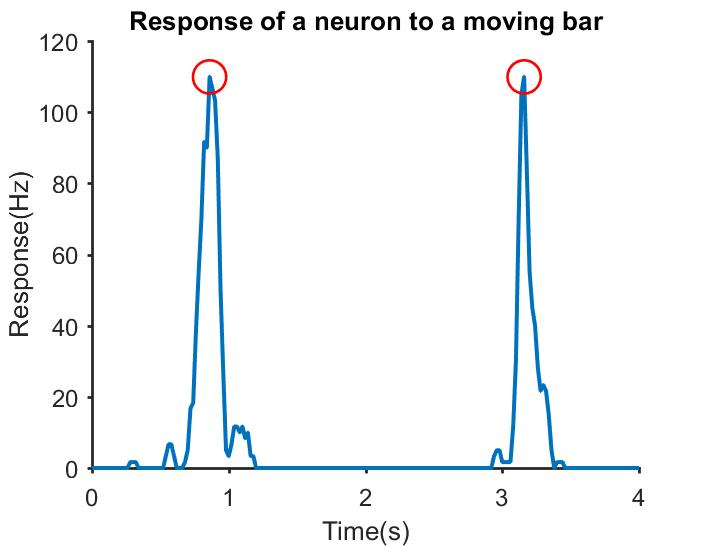
\includegraphics[width=\linewidth]{methods/SDF_movingbar.jpg}
		\caption{The SDF of a neuron’s response to a vertical bar moving bidirectionally. The maximum response in each direction is highlighted with red circles}
		\label{fig:mb}
		\end{figure}

	When shown gratings, neurons respond differently. A neuron, based on whether it demonstrates linear summation over its receptive field or not, responds differently to a grating. For example, ‘linear’ cells give a response modulated to the temporal frequency of a grating (see Figure \ref{fig:fourier}a; TF= 4Hz). A Fast Fourier Transform of the SDF is taken (Figure \ref{fig:fourier}b) and the peaks observed indicate that the respective frequencies have a high magnitude in the original signal. In this case, the FFT has two distinct peaks (red circles), the first one is at 0 Hz and the second one at 4Hz. The peak at 0 Hz is the F0 component of the response and is equal to the average of the signal in figure \ref{fig:fourier}a. The second peak is the F1 component and gives the fundamental frequency of the neuron’s modulated response (4 Hz). ‘Non-linear’ cells don’t show a modulated response to gratings, especially for higher spatial frequency gratings and as a result, the only distinct peak in the FFT corresponds to the F0 component (0 Hz). 
			\begin{figure}[H]
			
			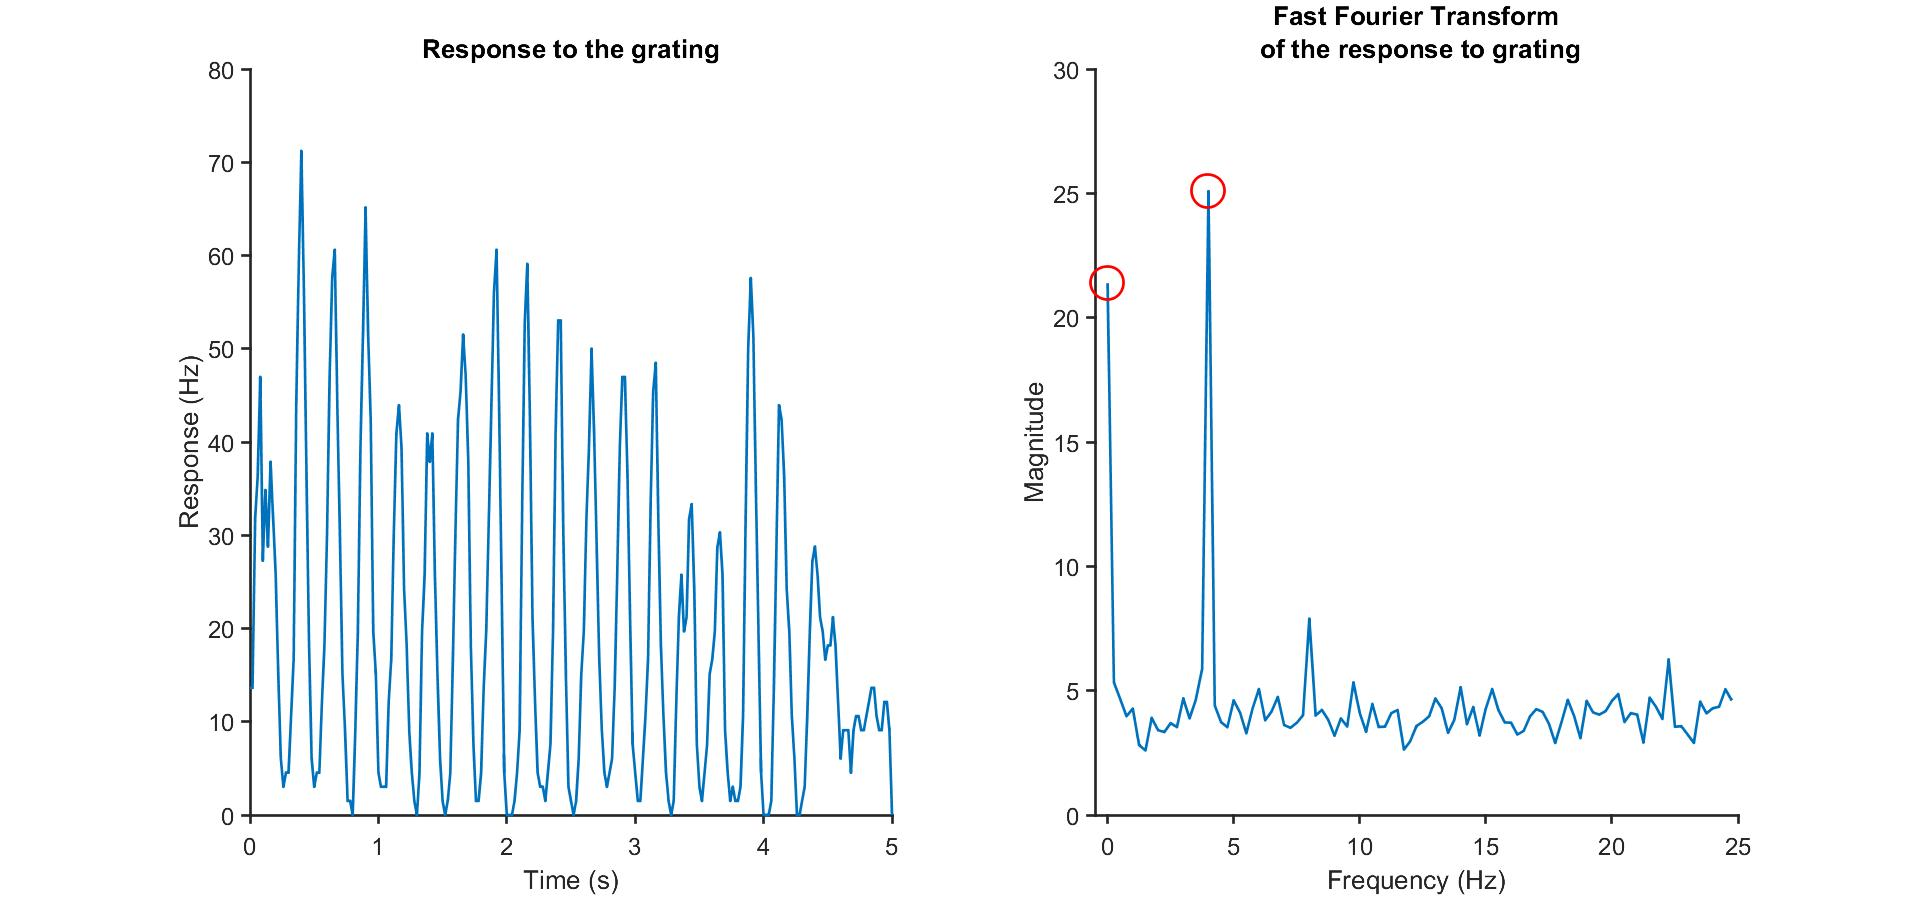
\includegraphics[width=\linewidth]{methods/Fourier.jpg}
			\caption{a) the SDF of a ‘linear’ cell. The first 4.3s was the stimulus presentation duration. A blank screen was presented for the last 0.7s. b) The fast fourier transform (FFT) of the signal in fig\ref{fig:fourier}a. There is a peak at the F0 component as well as at 4 Hz, which was also the temporal frequency of the sine wave grating.}
			\label{fig:fourier}
			\end{figure}
	
	Cells were first classified as linear or non-linear neurons – with our cortical and collicular data, comparable to the classical categories of simple and complex in the primary visual cortex (Hubel and Wiesel , 1962) and X and Y like in the lateral geniculate nucleus (Enroth-Cugell and Robson, 1966). This was done by taking the modulation index (Skottun et al., 1991) which is the ratio of the F0 and F1 components of the response. Traditionally, the modulation index is calculated by dividing the F1 component of the response by the F0 component. Neurons with modulation index less than 1 were classified as non-linear cells and cells with modulation index greater than 1.5 were classified as linear cells. Recently, a modified measure of the modulation index was proposed to measure linearity in the tree shrew primary visual cortex (Van Hooser et al., 2013). Using this measure, the range of values the modulation index could take was between 0 and 2 where neurons with modulation index less than 1 were classified as non-linear cells and where neurons with modulation ratio between 1 and 2 were classified as linear cells. This measure of modulation index was chosen to enable comparison with earlier tree shrew studies. For non-linear cells, the F0 component of the response was used for further analysis while for linear cells, the F1 component was used. From the response of the neuron to drifting sinusoidal gratings of increasing spatial frequencies, the spatial frequency tuning curves of the neuron was constructed and the peak spatial frequency and the half width at half height were calculated.
	
	\section{Histology}
	
	After the experiment, the tissue was processed for histology as follows. The brain was stored in a 25\% sucrose solution until it sank. This was to ensure that the tissue was cryoprotected. The brain was cut into blocks so that only the areas of interest were sectioned. The brain was frozen and 50 micron sections were made using a cryostat (Leica CM3050S, Leica Microsystems, Nussloch, Germany). The sections were collected and stored in a Sodium Azide solution (0.1\% in 0.1M PB) till they could be mounted on gelatinised slides after which they were dried overnight and stained.
	
	\subsection{Cresyl violet staining}
	
	First the sections were dehydrated using increasing concentrations of ethanol solution. Then, chloroform was used to de-fatten the sections. This was followed by rehydrating sections in decreasing concentrations of ethanol. The sections were then stained using Cresyl Violet Acetate solution (0.1\%, Sigma-Aldrich, Inc., USA) and differentiated using a solution of 5\% percent acetic acid in 95\% ethanol. The sections were then fixed in histolene and the slides were coverslipped.
	
	\subsection{Track Reconstruction}
	
	In order to reconstruct electrode tracks, the electrolytic lesions were located under a light microscope and digitised (Zeiss Axiocam Digital Camera, Zeiss, Germany). The shrinkage was calculated by comparing the recorded and observed distances between lesions using Adobe Illustrator(Adobe systems software Ltd). The shrinkage calculation was used to accurately determine the actual depth of the units recorded. In tree shrew V1, based on the location of the unit, it was classified as layer 4 or layer 2/3. In the shrew superior colliculus, the units were categorized as either belonging to the superficial or deeper layers of the superior colliculus.
	
	\section{Optical Imaging of Intrinsic Signals}
	
	Optical imaging of intrinsic signal is a high resolution imaging method that is used to detect the changes in blood oxygenation level in areas of neuronal activity. As a result of neuronal activity there is increased oxygen consumption in the surrounding tissue which leads to an increase in the level of de-oxy haemoglobin in the blood. This leads to a difference in reflectance in the tissue between regions where there is oxygenated and de-oxygenated blood and it is this signal that OI detects. This is the same signal as the fMRI BOLD signal but optical imaging has one key advantage over BOLD imaging. Whereas the fMRI signal has the resolution in the scale of millimetres, OI can detect  signals at at least one order of magnitude higher resolution, allowing us to visualize the organization of neuronal activity at the scale of cortical columns. So, Optical imaging was used to image the functional activity of the macaque primary visual cortex. 
	\subsection{The apparatus}
	
	In order to acquire OI maps of the primary visual cortex, first, a tandem lens macroscope was attached to a slow-scanning CCD camera. A light source is used to provide illumination for the duration of the imaging and the acquired frames were converted into a digital signal using an analog to digital converter. The specifications of these equipments are detailed below.
	
	\subsubsection{Macroscope and camera}
	
	A tandem lens macroscope was constructed by arranging two camera lenses (Pentax lenses, f= 50mm) end-to-end. This macroscope had a shallow depth of field which allowed us to focus at a specific depth below the surface of the cortex. In this manner, we acquired the blood flow changes related to the neuronal activity at the depth where the lens was focused. The macroscope was connected to a slow scan CCD camera (Teli CS 8310B; Ts’o et al., 1990) which acquired and transmitted images to the imaging system (VDAQ Imager 3001, Optical Imaging, Rochester, NY). 
	
	\subsubsection{The Chamber}
	
	As the images were acquired in-vivo in an anaesthetized macaque, there was the possibility of the image being contaminated by movement artefacts caused by the animal’s respiration and heartbeat. To reduce this, a metal chamber (diameter= 10 mm) was placed on the skull surrounding the exposed cortical area. It was sealed in place using dental cement (Dentimex VA, Netherlands) and ensured that no leaks were present. Once the chamber was fixed to the skull, it was filled with Silicone oil (Polydimethylsiloxane 200 fluid, viscosity 50 cSt, Sigma-Aldrich, Inc., USA) and sealed with a coverslip. In the macaque, due to the angle of the imaged area, we used a metal chamber without the metal pipes traditionally used to fill the chamber. The cylinder was overfilled with Silicone oil and the coverslip tightened. Where bubbles were present, the process was repeated until a clear view of the cortex was achieved.
	
	\subsubsection{The Illumination System}
	A circular fibre-optic attachment was connected to the camera lens for uniform illumination during optical imaging. First, a green light filter (545 nm) was used to obtain an image of the cortical surface with blood vessel landmarks (the green image). Then a longer wavelength (630 nm) filter was used for imaging. This wavelength of light was used because it was shown to reliably isolate the haemodynamic changes related to neuronal activity. Shorter wavelength lights (< 600 nm) reveal more of the blood volume changes while light of wavelength longer than 630 nm primarily detected light scatter effects. Light at 630 nm was the longest wavelength of light we could use to ensure maximum penetration of the light into the cortex while still imaging the haemodynamic changes.
	
	\subsection{Image acquisition}
	
	\subsubsection{Stimulus presentation}
	
	Stimulus was generated by the ViSaGe system and displayed on the BARCO monitor as described below. The Visage and the camera were synchronized by the means of an optical imaging interface (VDAQ Imager 3001, Optical Imaging, Rochester, NY). The interface started the camera when the stimulus presentation began. The stimuli were eight full field, bidirectional, square wave gratings (contrast =100\%; Spatial Frequency = 1-2.5 cycles/degree; Temporal Frequency = 1.5 Hz) of changing orientations. The stimulus was presented for 7.2 seconds, followed by a 10 second blank. This inter-stimulus interval allowed the OI signal to return to baseline. This was repeated 50 times to improve the signal-to-noise ratio.
	
	\subsubsection{Image acquisition system}
	
	The macroscope was focused below the surface of the cortex between 550 and 700 μm. Then, when the stimulus was presented, the Imager 3001 simultaneously started the camera which acquired 18 frames, each 400 ms long while the stimulus was presented. There was no image acquisition during the inter stimulus blank time. In order to get an image of the cortex at rest, a blank stimulus was presented for 7.2 s, followed by a 10 s interstimulus interval. The camera had a 14-bit bit-depth, which allowed the detection of very small variations in the OI signal. The individual frames for each block (10 trials per block) were first saved by the imaging system and exported to MATLAB for further analysis.
	
	\subsection{Analysis of Intrinsic Signals}
	
	\subsubsection{Pre-processing of the data}
	
	Prior to the analysis, the data acquired had to be corrected for luminance artefacts. We did this by averaging frame numbers 3 to 16 from all the 50 trials for each stimulus condition (between 1200 and 6800 ms) and dividing it by the average of the first frame across 50 trials. These frames were chosen as the signal from OI when using the 630 nm light is biphasic (see figure \ref{fig:oit}). The initial signal first dips below the baseline and then increases later, peaking at approximately 5 s after the stimulus was presented. This is generally consistent with the time-course of the de-oxyhaemoglobin concentration (Malonek and Grinvald, 1996). To account for the illumination effects, the first frame subtraction method was employed to create a differential map. In this method, the blank was taken as the first frame and the activity of all other frames are calculated as the difference of the frame from the ‘blank’ frame. This division by the blank is equivalent to subtracting and dividing by the blank since the optical imaging signal is relatively small (see Pouratian \& Toga, 2002).
	
		\begin{figure}[H]
		
		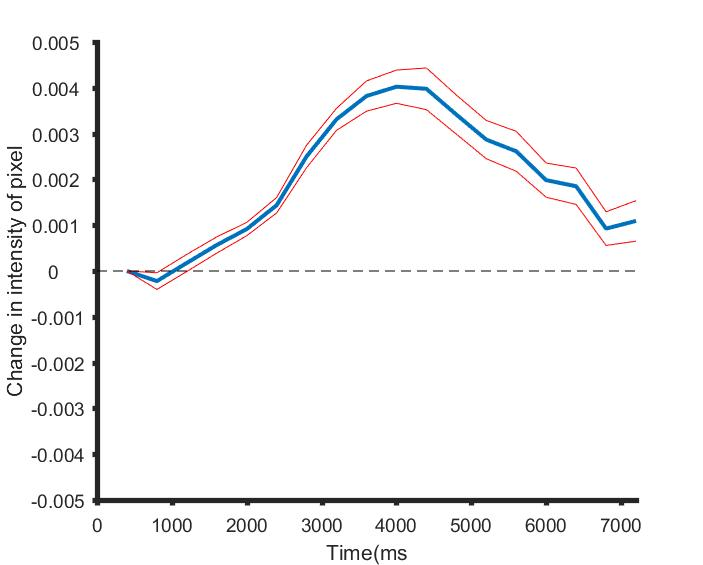
\includegraphics[width=\linewidth]{methods/OI_timecourse2.jpg}
		\caption{The time course of the OI haemodynamic signal for the duration of the stimulus presentation. The deoxyhaemoglobin levels briefly increase before decreasing, leading to a decrease in pixel intensity followed by an increase.}
		\label{fig:oit}
		\end{figure}
	
	\subsubsection{Obtaining single condition and orientation maps}
	
	The differential map is bandpass filtered in order to obtain the single condition map. This is done as follows. First the differential map is low pass filtered using a Gaussian kernel with a large sigma value (312.5 microns). The low pass filtered map is subtracted from the differential map to obtain the highpass filtered map which is once again filled with a Gaussian kernel with a small sigma value (100 microns). The resulting map is the single condition map (SCM; see figure 4).
	
	\begin{figure}[H]
		
		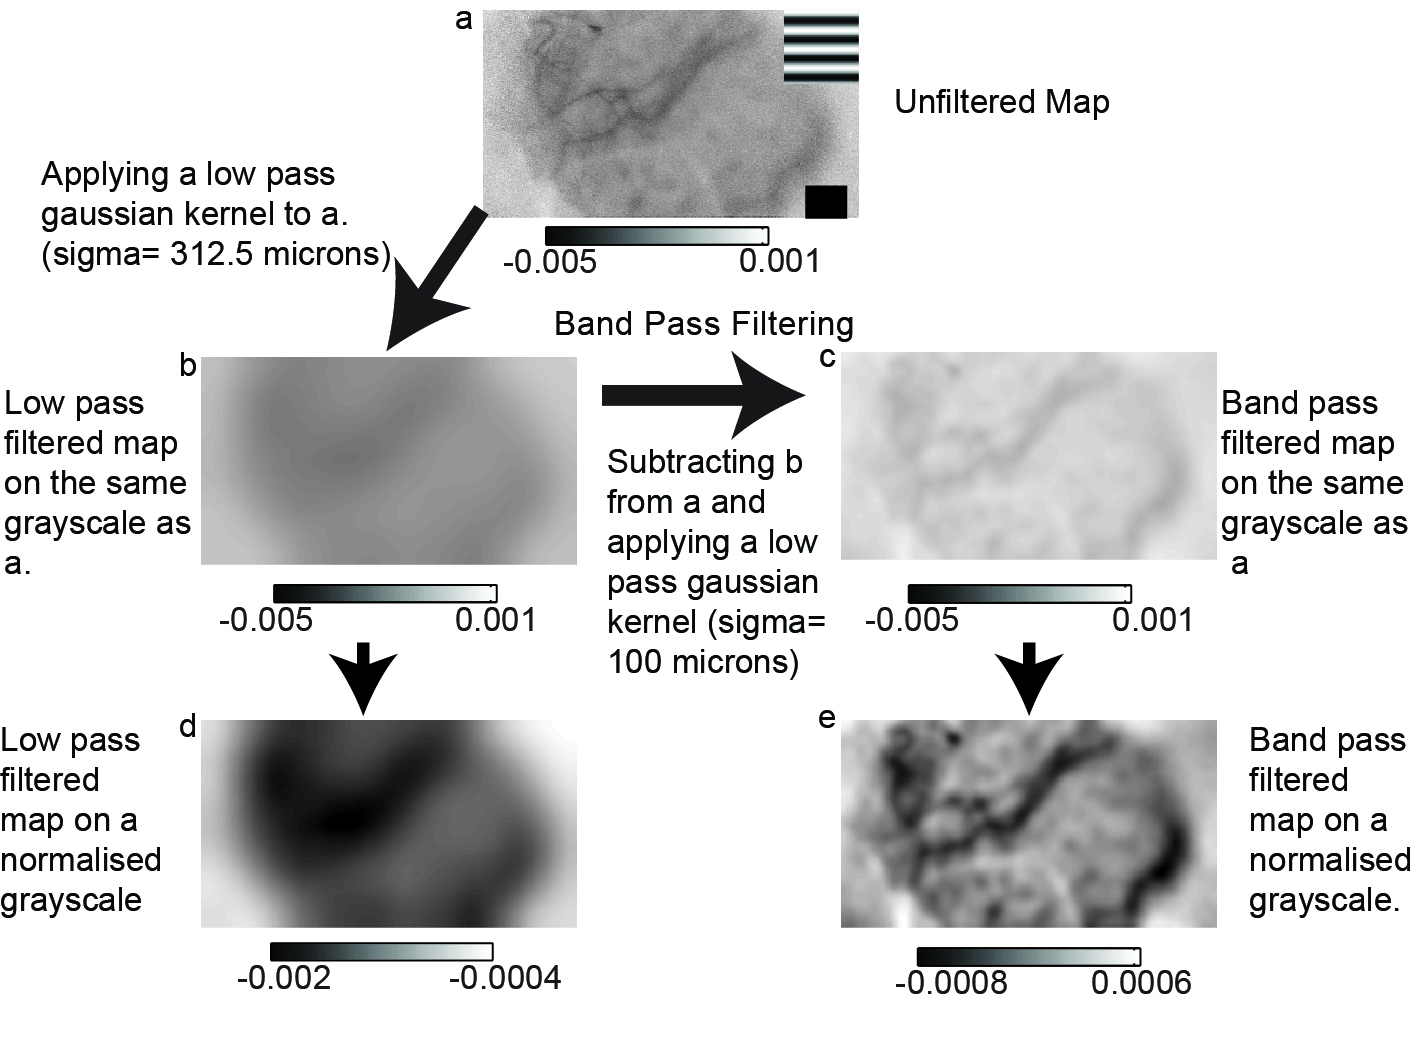
\includegraphics[width=\linewidth]{methods/filters.jpg}
		\caption{The filtering process used to generate single condition maps. The differential maps are first high-pass filtered to remove spatial scale signals and a smaller low-pass, smoothing filter was used to remove the high spatial noise.}
		\label{fig:filters}
	\end{figure}
	
	The single condition maps obtained for each orientation are then vector averaged (Swindale, 1998) to create the orientation domain map.
	
\chapter{Radial Bias in large spatial scale optical imaging signal in the macaque Primary Visual Cortex}

\pagebreak

	\section{Summary}
	
	Neurons in the primary visual cortex are tuned to orientation and similarly oriented neurons are arranged in columns, with orientation columns arranged like spokes around a pinwheel. The different orientations are however not equally represented. Two different types of biases have been reported in the representation of orientations in the primary visual cortex, namely the oblique effect and the radial orientation bias. Electrophysiological and fMRI studies have shown a preponderance of the radial orientation in the primary visual cortex of mammals. However, optical imaging of intrinsic signals (OI), which are related to the fMRI signals do not show this radial bias. Here, OI signals on a spatial scale comparable to that of the fMRI signals were examined. The orientation selectivity of the spatially unfiltered, raw signal obtained from OI was compared to the radial angle and a significant radial bias was found in this signal. When a similar analysis was performed on a traditionally band-pass filtered OI signal, a much weaker radial bias was found. As the OI signal is predominantly due to synaptic and pre-synaptic activity, it is proposed that the global signal in OI corresponds to cortical inputs. If the cortical inputs are biased for only a small number of orientations, then this provides evidence for a model of orientation selectivity where orientation tuning of cortical neurons are sculpted from orientation biases encoded in a small number of broadly tuned channels.
			
\pagebreak

	\section{Introduction}
	
	Neurons in the primary visual cortex are tuned to orientation and the orientation tuned neurons are organised in columns. Hubel and Wiesel (1962) showed that neurons in Area 17 of cats were sharply tuned to orientation. These neurons were also grouped into neurons of similar orientation. Optical imaging studies in the cat A17 and 18 showed that the cortical orientation columns were organised as the spokes of a pinwheel, converging on the pinwheel centre (Bonhoeffer and Grinvald, 1991; Grinvald et al., 1986). Models of orientation selectivity and cortical architecture assume that neurons are equally tuned to all line orientations. However, studies suggest that there is an overrepresentation of some orientations in the visual system. Two types of orientation biases have been demonstrated in the visual system. The first is the oblique effect, which manifests as an underrepresentation of the oblique orientations while the horizontal and vertical orientations are overrepresented (see Appelle, 1972 for review). The second is the radial bias; where neurons are preferentially tuned to the orientation parallel to the line joining the centre of the receptive field to the centre of the visual field (Levick and Thibos, 1980). Both these biases have been reported in the macaques.
	
	Where the relationship between the receptive field location and visual field locus were studied, a radial bias has been reported every time. Early studies of biases in orientation representation in the cortex reported a strong oblique effect in electrophysiological studies (Chapman and Bonhoeffer, 1998; Coppola et al., 1998; DeValois et al., 1982; Kennedy et al., 1985; Leventhal, 1983; Li et al., 2003; Mansfield, 1974; Mansfield and Ronner, 1978; Orban and Kennedy, 1981, Payne and Berman, 1983; Pettigrew et al., 1968); which was congruent to the findings of a prominent oblique effect in behavioural studies reported in most species, from humans to octopuses (Appelle, 1972; Campbell et al., 1966; Furmanski and Engel, 2000; Rovamo et al., 1982). However, these studies examined the orientation preferences of neurons without studying their corresponding receptive field locations. Later studies that characterised the receptive field location with regards to the visual field locus all reported a radial bias in almost all species that were studied using electrophysiological studies (Levick and Thibos, 1980; Levick and Thibos, 1982; Maloney et al., 2014; Passaglia et al., 2003; Leventhal, 1983; Leventhal and Schall, 1983; Smith et al., 1990; Vidyasagar and Henry, 1990; Schall et al., 1986a; Schall et al., 1986b, Shou and Leventhal, 1989), fMRI imaging studies (Sasaki et al., 2006; Swisher et al., 2010; Mannion et al., 2010) and behavioural studies where subjects observed natural scenes instead of oriented gratings (Hanson and Essock, 2004).
	
	One of the key tools that have been instrumental in revealing cortical architecture is optical imaging of intrinsic signals (OI). Using OI, not only have the ocular dominance domains and orientation domains been visualised, but their relationships with each other have also been examined (Bartfeld and Grinvald, 1992). The haemodynamic change accompanying neural activity that is recorded using OI is akin to the BOLD (Blood Oxygen Level Dependent) response observed in fMRI (Menon et al., 1995; Logothetis et al., 2001). While the orientation biases studied using the fMRI BOLD responses reveal a radial orientation bias, only the oblique effect has been reported using OI (Chapman and Bonhoeffer, 1998; Coppola et al., 1998; Grabska-Barwinska et al., 2009).
	
	One reason for this discrepancy in these findings could be due to the spatial scale at which these signals are studied. The BOLD signal has a poorer spatial resolution compared to the OI signals, which is capable of resolving cortical columns (Churchland and Sejnowksi, 1988). The BOLD and OI responses predominantly consist of the pre-synaptic and synaptic activity with the extracellular, spiking activity forming a fairly small part of the response (Logothetis et al., 2001). Traditionally, images obtained using OI are band-pass filtered to reflect activity corresponding to a narrow spatial scale (between 100-500 microns). While this spatial filtering has the advantage of isolating the weaker, smaller spatial scale spiking activity, it has the disadvantage that by omitting the larger spatial scale activity, any information present at this spatial scale is lost. Here, we aimed to use the unfiltered larger spatial scale signal. We hypothesised that when this larger spatial scale signal is studied in the anaesthetised macaque striate cortex, we will find a bias for the radial orientation as has been reported in the fMRI studies. 
	
		
	\pagebreak
		
	\section{Methods}
	In this study, we imaged and recorded from the cortex of five, anaesthetised male macaques (Macaca nemestrina, 2-4 years old). All experimental procedures were approved by the Florey Institute of Neuroscience and Mental Health Animal ethics committee and conformed to the guidelines of the National Health and Medical Research Council’s Australian Code of Practice for the Care and Use of Animals for Scientific purposes.
		\subsubsection{Surgery and anaesthesia}
		Surgical procedures were as described in the methods section. Briefly, animals were anaesthetised using a Ketamine/Xylazine mixture (Ketamil, 15mg/kg, i.m., Parnell Laboratories, Australia; Cylazil, 2mg/kg, i.m., Troy Laboratories, Australia). Venous cannulation was performed on the cephalic vein to administer fluids and paralysant (Norcuron, initial bolus of 0.7 mg/kg followed by 0.2 mg/kg/hr, Organon Australia Pty Ltd) to the animal and a tracheostomy was performed to administer the anaesthesia (0.5-2\% Isoflurane in a mixture of nitrous oxide and oxygen (70:30)) during the experiment. The animal was placed in a stereotaxic frame and its head fixed using ear bars. During the experiment, the end-tidal CO2 (3.6-3.8\%), electrocardiogram, electroencephalogram and the core body temperature were all monitored. A craniotomy and durotomy were conducted over the location of the primary visual cortex (Horsley-Clarke co-ordinates: 24-34 mm posterior and 2-10mm lateral). The eyes were dilated by applying 0.1\% Atropine (Sigma Pharmaceuticals Pty Ltd, Australia) and rigid, gas permeable lens were introduced to prevent corneal drying and optical lenses and artificial pupil (4mm) were used to correct any refractive errors and reduce optical aberrations.
	
		\subsubsection{Optical Imaging of Intrinsic Signals}
		
		\paragraph{Setup}
		Optical imaging of intrinsic signals was used to obtain the haemodynamic change related to the neural response to orientation stimuli. The OI setup involved two camera lenses (2 x Pentax lenses, f=50 mm) arranged in a tandem fashion (Frostig et al., 1990) connected to a CCD camera (Teli CS8310B). The tandem lens arrangement allowed us to choose a narrow plane of focus. An LED light source was used to illuminate the cortical surface. Before stimulus presentation, a high contrast, ‘green image’ of the surface of the cortex was obtained by illuminating the cortical surface with a green light (filter wavelength=545 nm). This provided us with cortical landmarks which were later used in determining the locations for electrode tracks of topographical recordings. Following this, the camera was focussed between 550-700 microns beneath the surface of the cortex and a red light filter (wavelength =630 nm) was used to illuminate the cortex. 
		
		\paragraph{Stimulus and data collection}
		
		During the experiment OI maps were obtained in response to visual stimulation. Visual stimulus was generated using the visual stimulus generator (SDL, Cambridge Research Systems, UK) and presented on a Barco monitor (Reference Calibrator plus; Barco Video and Communications, Belgium).  The monitor was positioned at 57 cm from the animal. The stimulus presented was a full field, square-wave, bidirectional, drifting grating (SF= 1-4 cpd, TF= 1.5 Hz, Contrast= 100\%). The orientation of the grating changed sequentially in 22.5 degree steps from zero to 157.5 degrees. A zero degree grating was a horizontal grating moving bidirectionally. The stimulus was presented for 7.3 seconds followed by an interstimulus interval of 10 seconds where the animal viewed a blank screen. 18 frames, each 400 ms long were collected for each stimulus presentation. The signal to noise ratio was enhanced by acquiring data over 50 trials collected in 10 blocks of 5 trials each. Where possible, given the condition of the imaged area and the animal, the experiment was repeated for a second time. Using the OI data acquisition system, each block was exported as a MATLAB® file. Each individual frame in a block was the average of that frame over 5 trials. Analysis was conducted on the exported MATLAB files.
		
		\paragraph{Image Analysis}
		
		Of the 18 frames collected, the mean of 14 frames (frames 3-16) was calculated for individual blocks in each stimulus condition. The first frame was then subtracted from the averaged frames for each stimulus condition. The mean of 10 blocks was then calculated. This gave us the unfiltered single condition maps (unfiltered SCMs). Traditionally, when analysing the images obtained using optical imaging of intrinsic signals, the unfiltered SCMs are band pass filtered using the method described in figure (Refer to method figure). The unfiltered map is first low pass filtered using a large spatial filter (Gaussian filter, sigma= 312.5 microns). This removes the low frequency information. By subtracting this low pass image from the original image, we preserve only the high spatial frequency information (high-pass SCMs). The high pass SCM is then smoothed with a gaussian filter with a smaller sigma value (100 microns). This is the band pass filtered single condition map or more commonly just referred to as the single condition map (these will be referred to as filtered SCMs throughout this thesis). The filtered SCMs are then vector averaged to look at the angular mean of individual pixels (Swindale, 1988). This will produce the traditional filtered orientation tuning maps. In our study, we also vector averaged the unfiltered SCMs. We called the maps derived this way the unfiltered orientation maps.
		
		\subsubsection{Topographical recordings}
		High impedence tungsten microelectrodes (6-12 MOhm, FHC Inc, ME) were used to record from predetermined locations on the imaged cortical surface. The analog signal was amplified and filtered (AM Systems model 1800, Washington; Gain = x10,000; Band pass between 300 and 3000 Hz). The filtered signal was then visualised using an oscilloscope and fed through an audio speaker to aid in plotting the receptive fields. First the foveal location (if visible) and the optic nerve with blood vessel markers were plotted using a back-projecting fundus camera. Then the locations of the receptive fields were carefully hand plotted using handheld stimuli from at least 3 locations in the imaged area. In between each electrode penetration, where possible, the location of the fovea and optic nerve head were replotted in order to account for eye movement. At six locations, the signal obtained from the electrodes and the filtered signals were digitzed (12.5 - 22.5 kHz, CED; Cambridge Electronic Systems, UK) and stored for later analysis.
		
		\subsubsection{Multi-electrode array recordings}
		In one animal, we used a 16 channel, linear, multi-electrode array (NeuroNexus Technologies Inc, USA) to record from the cortex. The array was inserted at an angle within the supragranular layers of V1. The individual electrode on the multielectrode array were separated by 100 microns. The array was connected to a pre-amplifier (RA16PA, Tucker-Davis Technologies, USA) through a headstage (RA16AC). The signal was amplified (x 10000) and filtered (2.2 Hz- 7.5 kHz) was applied and the resultant signal was digitized (12.5kHz) using the OpenEx software (TDT, USA). The digitized signal was further digitally filtered between 2.2Hz and 100 Hz, and down-sampled to 1017.3 Hz to obtain the LFP signal and between 300-3000 Hz to obtain the multi-unit recordings.
		
		\subsubsection{Stimulus for electrode recordings}
		To make topographical recordings, a handheld stimulus was used. The orientation, direction and speed of the stimulus movement were all varied so that the neuron was ideally stimulated. Following this, the receptive fields of the neurons were hand-plotted and used for further analysis.
		
		For the single electrode recordings and linear array recordings, a bi-directional moving bar (10o x 0.5o bar, contrast = 100\%, speed= 2.5- 5o/s), whose orientation changed incrementally from -90o in steps of 20o was used. The responses were recorded for 9 orientations with bars moving in 2 directions (a total of 18 directions) over 10 trials. The monitor used to present the stimuli and software used to generate the stimuli were the same as described for optical imaging.
		
	\subsubsection{Data Analysis}
	
		\paragraph{Analysis of electrophysiological recording}
		
		For both the single electrode and the linear array recordings, multi-unit activity and LFPs were analysed to get the optimum orientation at a recording site. For recordings made using single electrodes, the Spike 2 software (Cambridge Electronic Systems, UK) and for linear array recordings, the Open Ex Software (TDT, USA) were used to apply digital filters to separate the signals into LFP (between 20 and 70 Hz) and multiunit activity (between 300-3000 Hz).  The LFP signal corresponding to each stimulus direction was averaged across 10 trials using custom code written in MATLAB. The difference between the peak and the trough of LFP signal at each orientation, over the location of the receptive field, was the maximum response at this orientation. These values were used to generate the polar plots and calculate the circular mean (as calculated by Swindale, 1998; See Appendix for code) at each of the recording sites. For multi-unit activity, a threshold was placed using the spike 2 software and any spike the was greater than this signal was collected into PSTHs and SDFs were made. The peak firing rate at each direction of movement was used to generate polar plots and calculate the circular mean of the data.
		
		\paragraph{Determing radial orientation- receptive field locations}
		
		In order to determine the azimuth and elevation of receptive fields obtained during the experiment, the Cartesian co-ordinates of the foveal location was set as (0,0). The horizontal and vertical distances of the receptive field centre from the foveal location were calculated. The azimuth and elevation of receptive fields were then calculated as the horizontal and vertical angles subtended by the animals’ eyes to the receptive field centre. If there were eye movements during the experiment, (0,0) was re-assigned to the new foveal location. Receptive field locations were replotted in relation to foveal locations plotted closest to the recording in order to get as accurate a receptive field location as possible. This then allowed us to accurately determine the azimuth and elevation of the receptive fields.
		
		Using the receptive field locations thus calculated, we used the eccentricity, azimuth and elevation values to calculate iso-azimuthal and iso-elevation lines on the cortex. We used previously published magnification factor calculations in the macaque cortex (Dow et al.,1981) to calculate the magnification factor —degrees in visual space one would traverse if we moved 1 mm in cortical space and the inverse magnification factor; how far one needs to move on the cortex to traverse 1 degree in visual space, given the eccentricity of the receptive fields. These values were used to calculate the azimuth and elevation of points on the cortex that were spaced 15 pixels (375 microns) apart. The radial angle of each of the points was calculated given the azimuth and elevation of their RF locations and averaged to calculate the average radial angle of the imaged area.
		
		\paragraph{Defining a region of interest}
		As described above, the azimuth and elevation of points on the cortex that were 375 microns were calculated. 30 x 30 pixel squares around these points were defined as Regions of interest (ROIs). The difference between the average optimum orientation of the individual pixels in the ROIs and the radial angle of the ROI centre was calculated for both the unfiltered and filtered orientation maps (See fig\ref{fig:roi}).
		
			\begin{figure}[H]
			
			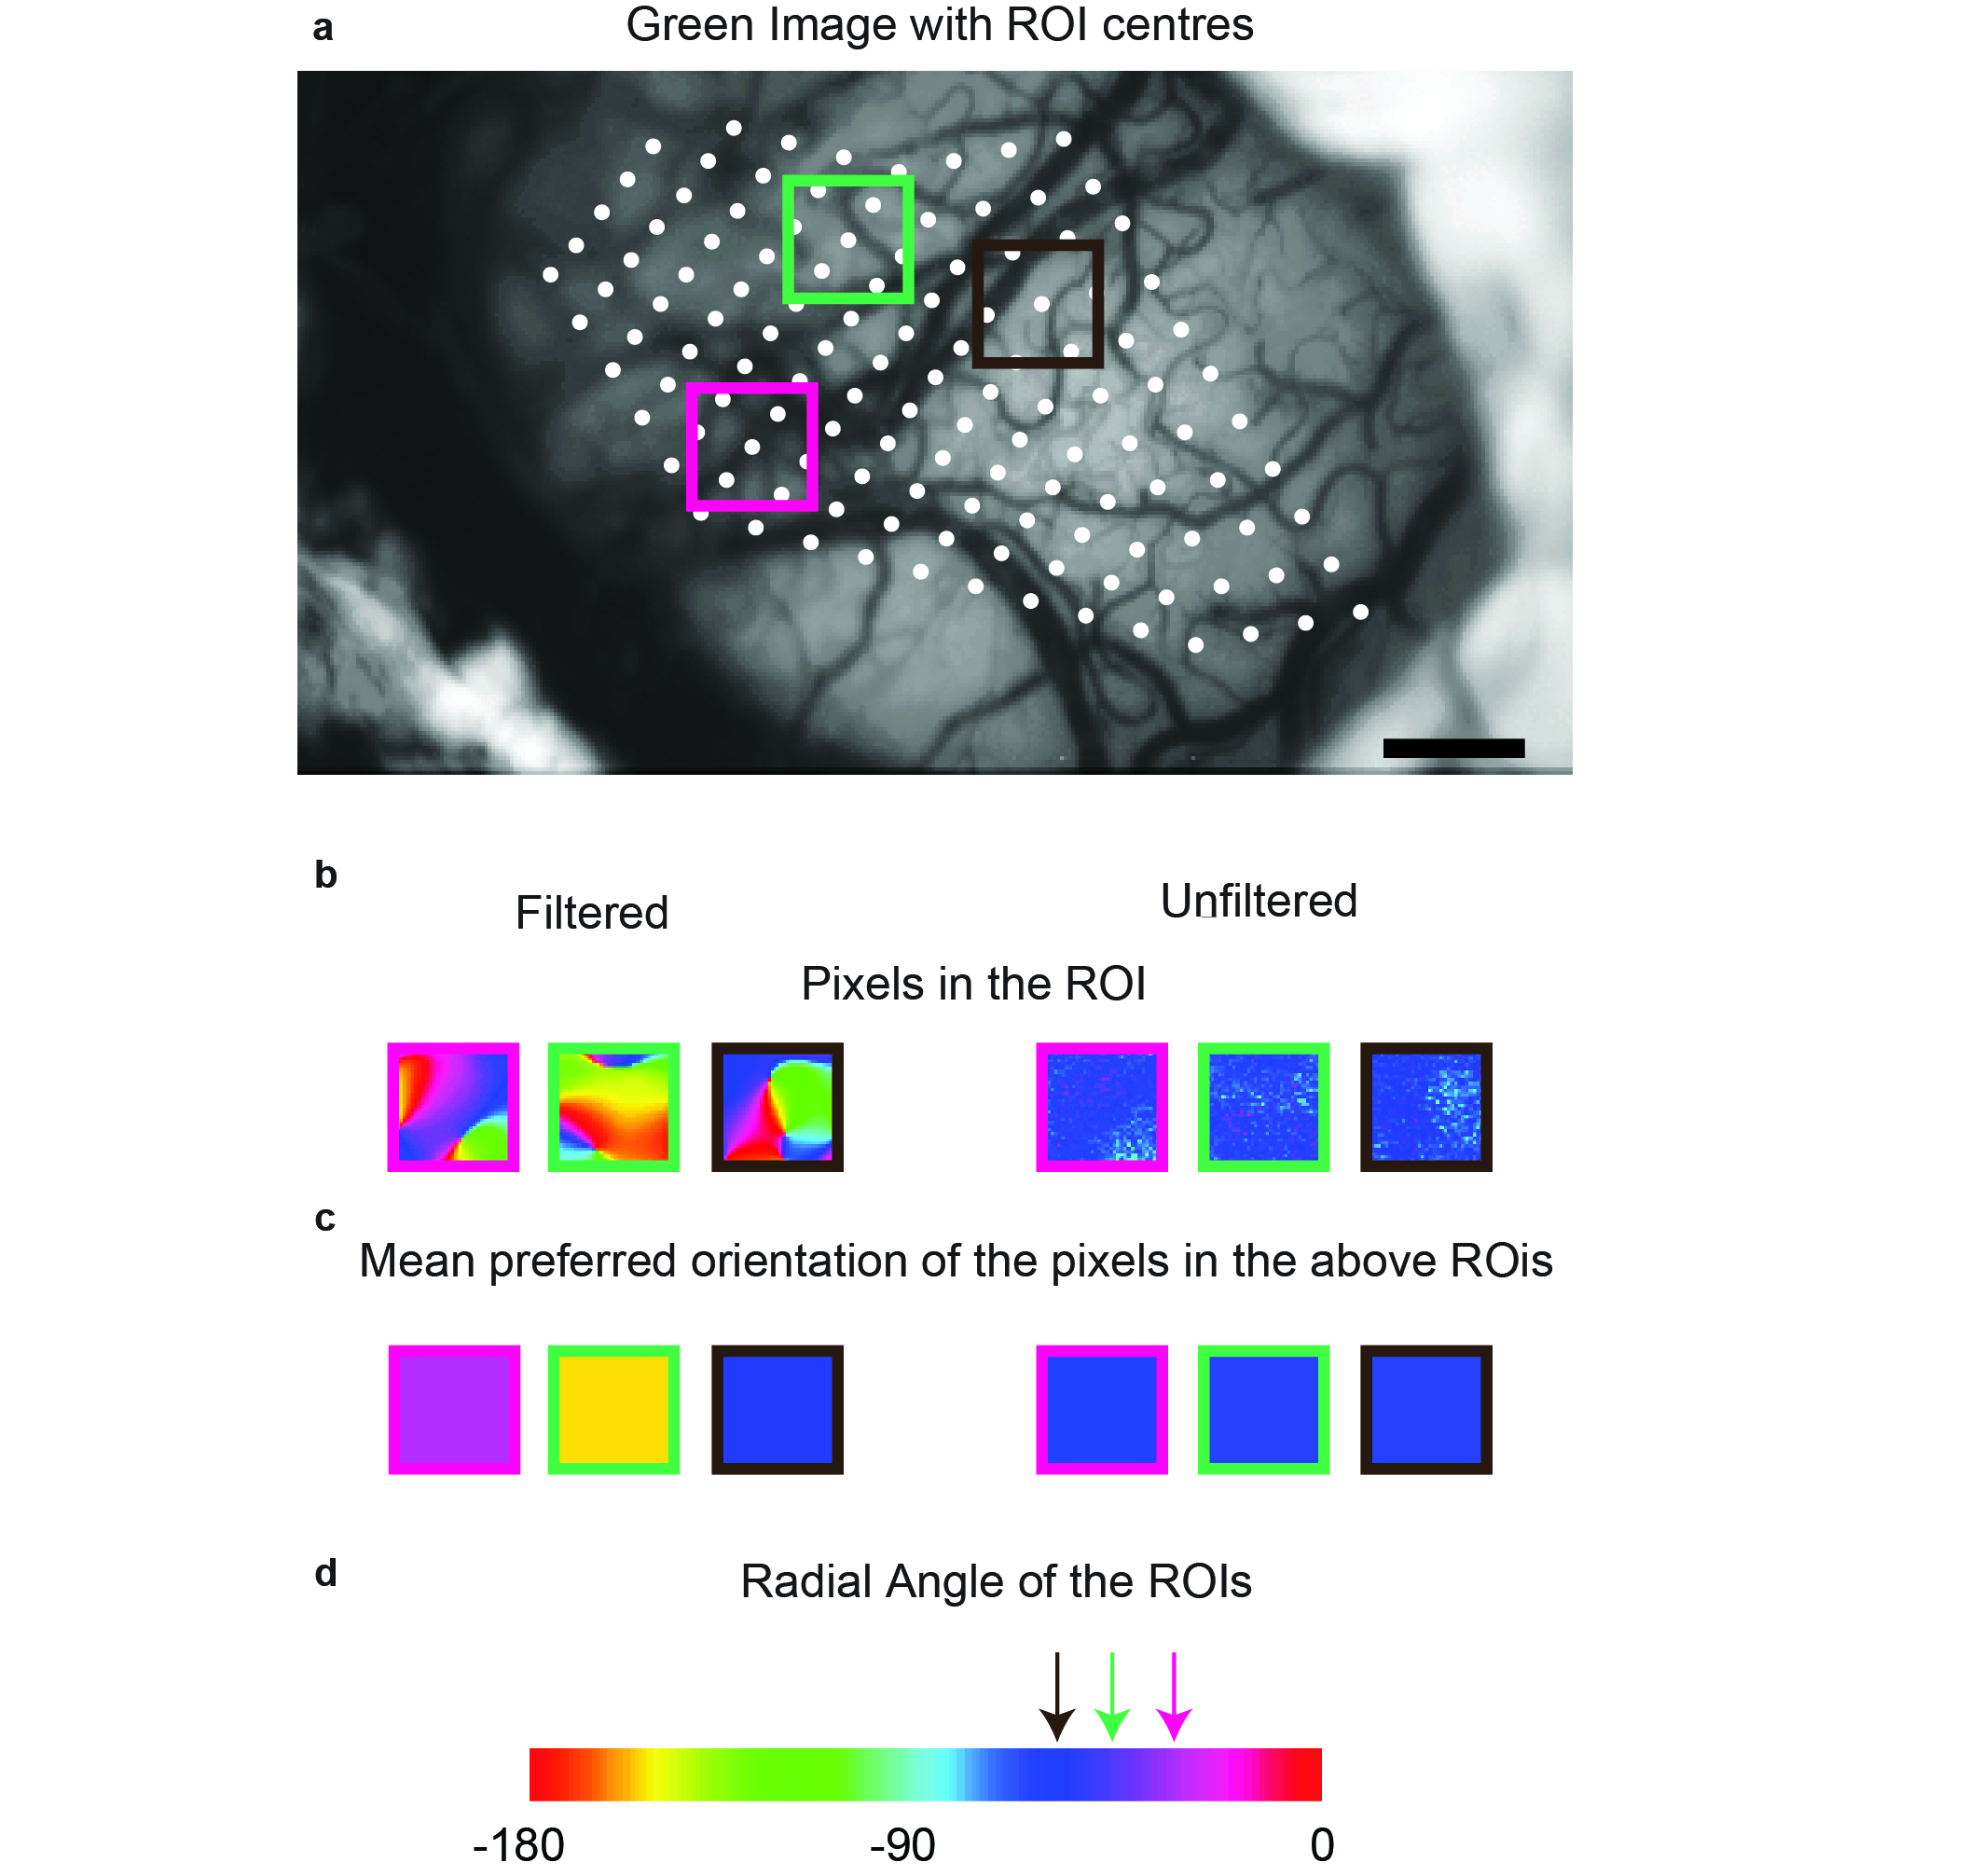
\includegraphics[width=\linewidth]{rb/FinalFigures/ROI.jpg}
			\caption{The generation of Regions of Interest (ROIs). a) the green image from the representative animal. The white dots are the centres of the ROIs. The ROIs were placed 15 pixels apart. Three ROI centres were randomly chosen and the region that is used for analysis is shown by the three coloured squares. b) shows the individual pixels in the filtered and the unfiltered conditions in the respective ROIs. c) shows the average orientation of the pixels in the ROIs. d) is the pseudo-color scale used to represent the different orientations in the orientation tuning maps and the pixels in the ROI. The three coloured arrows indicate the radial angle of the corresponding ROIs.}
			\label{fig:roi}
		\end{figure}
		
		\paragraph{Single Pixel Analysis}	
		
		The ROI analysis was used to determine if any of the cortical inputs were dominant in the larger spatial scale. To see if such bias was present at a single pixel level, we also compared the orientation tuning of single pixels to the radial bias of the imaged area. Accordingly, the optimum orientation of the individual pixels was subtracted from the mean radial orientation of the imaged area for the unfiltered and filtered maps. 
		
		\paragraph{Adjusting for sample size in single pixel analysis}
		
		During the single pixel analysis, individual pixels from orientation maps in five animals were examined. This amounted to a large number of pixels (10$^5$ pixels). In order to make sure we were not detecting an insiginificant effect made significant by sample size, we randomly resampled with replacement from the distribution of pixels in both the filtered and the unfiltered conditions to see if an effect could be observed at smaller sample sizes. We used two sample sizes (40 and 1000) sampled 1000 times and calculated the chi-square of the 1000 trials. The mean and the 95\% confidence intervals of the chi-square value from 1000 trials were calculated. If the upper limit of the 95\% CI of the chi-square value was lower than the 5\% critical value, then the distribution of the single pixel differences was not significantly different from a uniform distribution in the majority of trials. If the lower limit of the 95\% CI was higher than the 5\% critical value, then the distribution of the single pixel differences was deemed significantly different from a uniform distribution in the majority of trials.
		\pagebreak
		
	\section{Results}
		We recorded from 5 monkeys (Macaca fascicularis, all male, aged between 2 and 5 years). In 3 monkeys, we imaged and recorded from the left hemisphere and in the other 2, from the right hemisphere. In all animals, OI signals were first recorded from the respective hemisphere; following this, topographical recordings were made. In 2 macaques, LFP recordings were made using single electrodes and in one macaque, the multi-electrode, linear array was used for recordings.
	
		\subsubsection{Single Condition Maps}
		As a first step in processing the results of OI, SCMs were made. The SCMs for the unfiltered and filtered maps from one representative animal are presented in figure 2a and b respectively. The orientation of the stimulus is shown above the respective SCM. The SCMs show that there is more activity overall in orientations closer to the radial orientations (denoted by the star) in the unfiltered maps (i.e. the overall map is darker). No such trend is visible in the filtered maps. Distribution of the intensities of the pixels of inverted SCMs (So that darker pixels have a greater intensity value) are presented in figure 2c. The line above the boxplots indicates the range of radial orientations of the imaged area in this animal. As observed in the SCMs, there is a peak at the radial orientation in the unfiltered maps while the distribution of the filtered pixels show no such trend.
			
						\begin{figure}[H]
							
							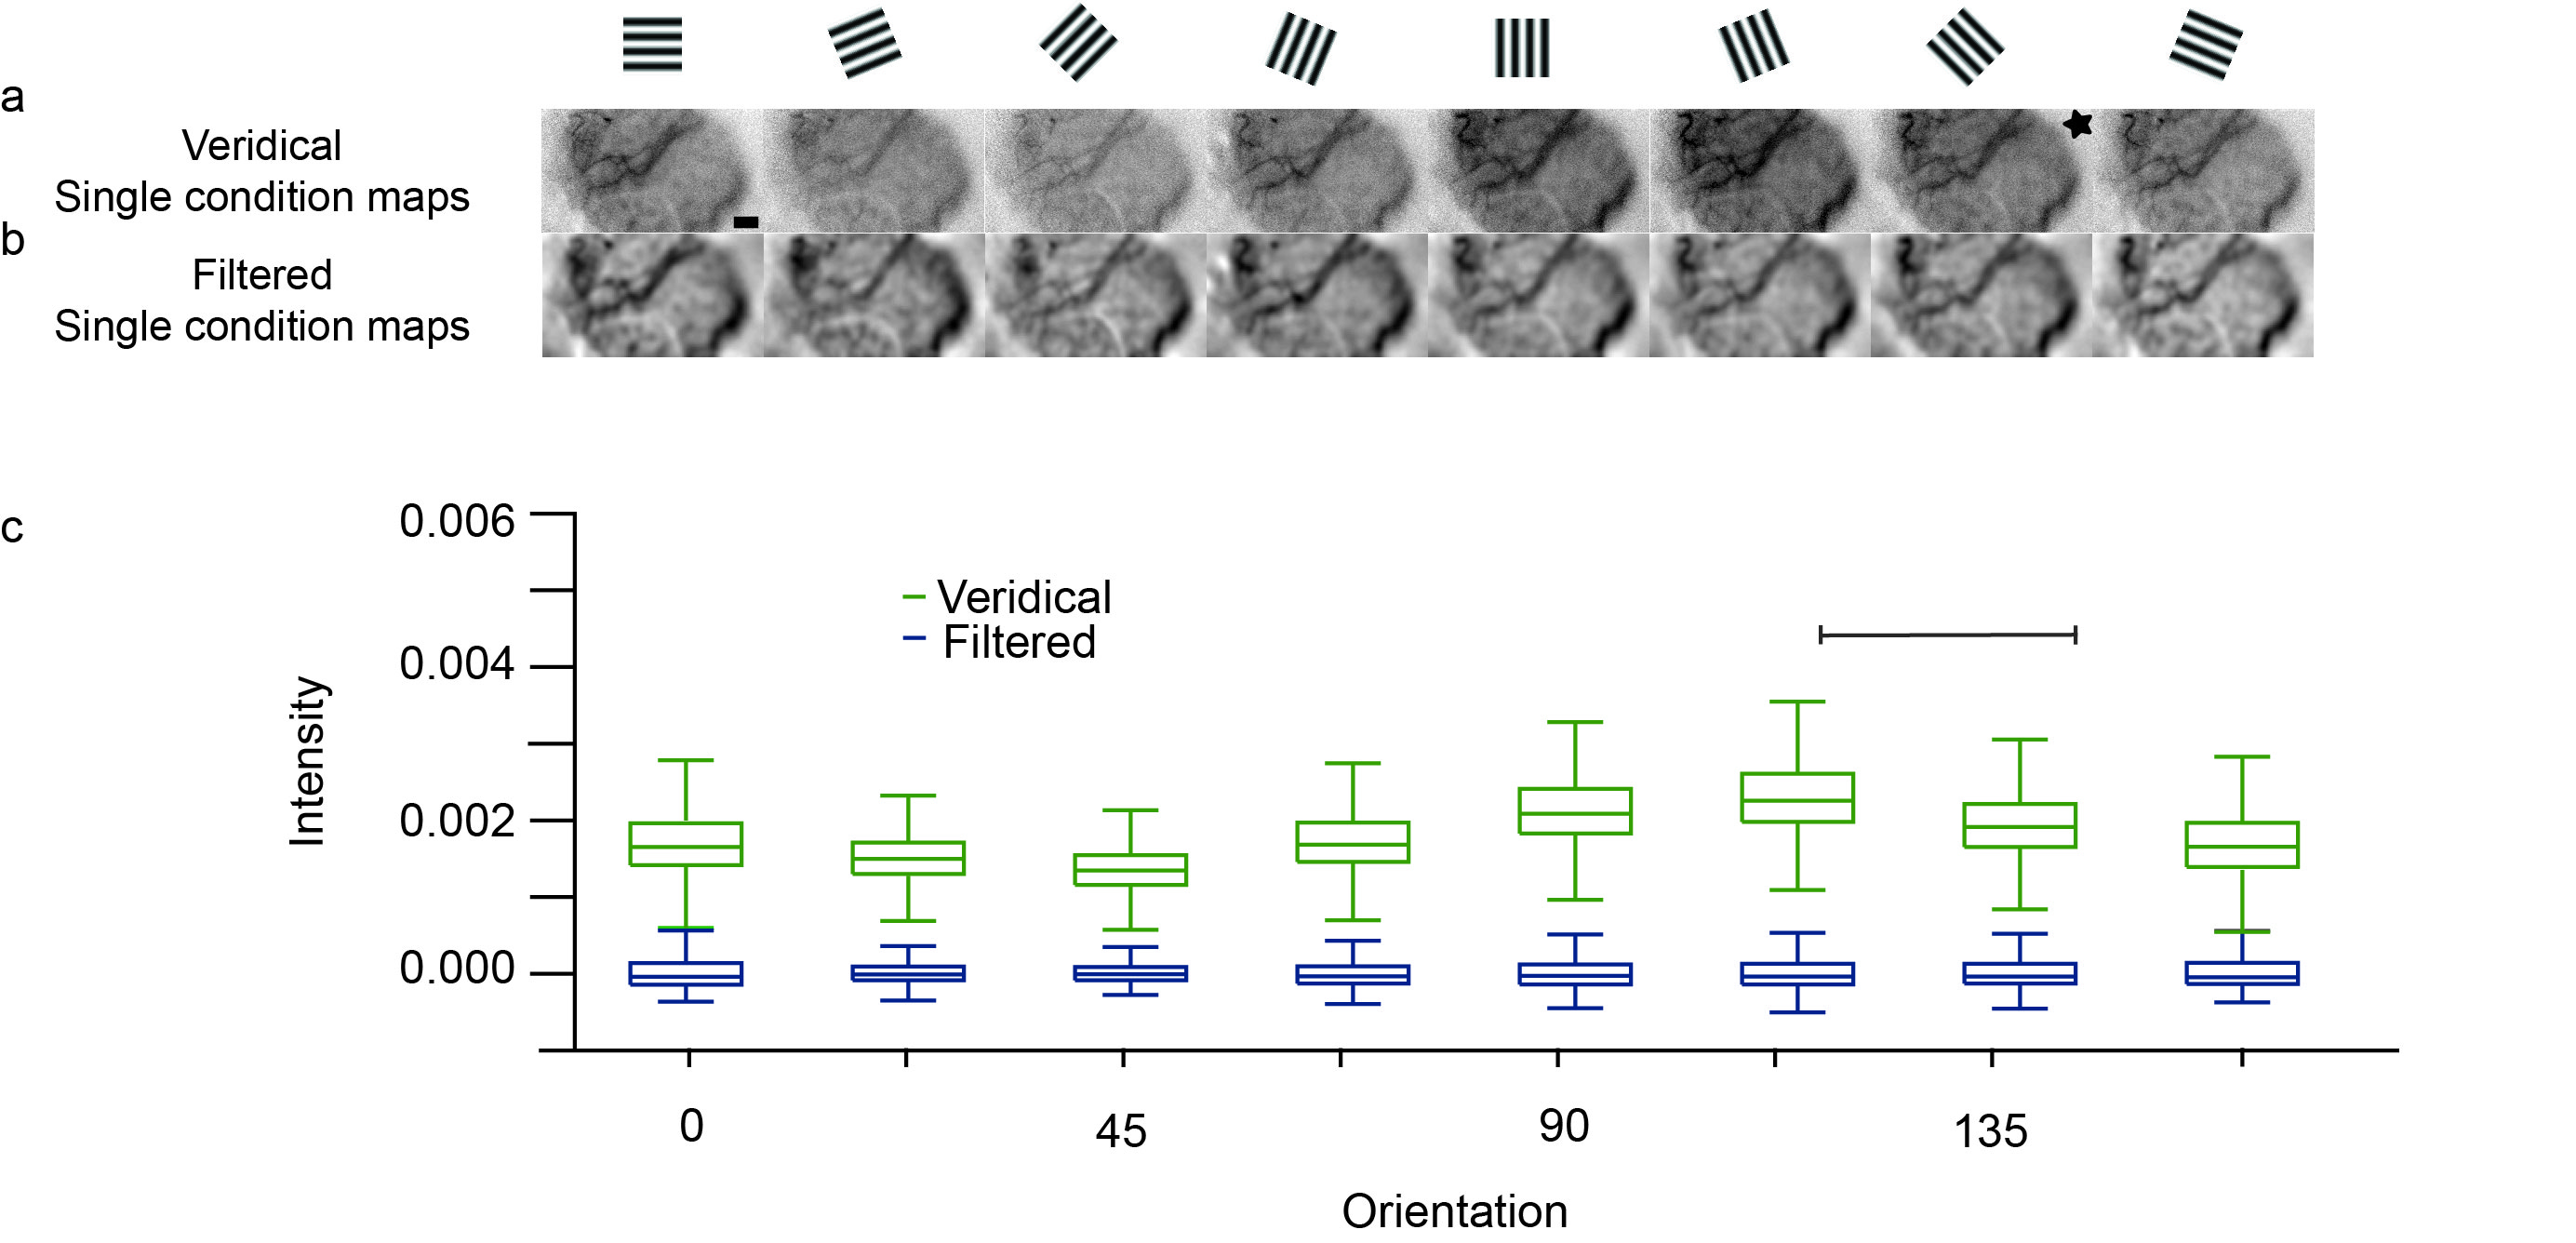
\includegraphics[width=\linewidth]{rb/scms.jpg}
							\caption{Distribution of pixels in unfiltered and filtered SCMs. (a) and (b) are the unfiltered and filtered SCMs. The stimulus orientation corresponding with each SCM is presented in the row above. The star denotes the orientation closest to the radial angle. Scale bar is 1mm. (c) is the boxplot of the distribution of the intensity of pixels in the unfiltered and the filtered maps. The line indicates the range of radial angles in the imaged area.}
							\label{fig:scm}
						\end{figure}
					
		\subsubsection{Orientation Tuning Maps}
			The unfiltered and filtered SCMs shown in figure 2a and b were vector averaged (Swindale, 1998) to produce the unfiltered and the filtered orientation maps in fig.\ref{fig:rep}. Figure \ref{fig:rep}a is the green image of the cortical surface with surface blood vessel landmarks. The different symbols correspond to the location of electrode tracks. The receptive field locations of the electrode tracks are shown in figure \ref{fig:rep}b. The polar plot corresponds to the orientation of a layer 2/3 neuron recorded from the location indicated by the diamond. The orientation of this neuron estimated using electrophysiological recording was 65.61$^o$; which was less than 22.5$^o$ away from the orientation of the neuron estimated using optical imaging was 86.89$^o$. The pseudo colour scale on the outside of the Cartesian scale is the same scale used in parts c and d. Figure \ref{fig:rep}c shows the filtered orientation maps and Figure \ref{fig:rep}d, the unfiltered orientation maps obtained during two repeats of the experiment. The filtered orientation map shows classical orientation domains that converge at a pinwheel centre, while the unfiltered orientation map is dominated by one orientation. This orientation corresponds to the radial orientation of the receptive fields in figure \ref{fig:rep}b; i.e. if we draw a line from the center of fixation to the center of the receptive field and extend it to the outer colour scale, we will observe the same colour as that seen in the unfiltered maps. Results for the unfiltered maps are presented in a similar fashion for all the animals in our study in figure 4.
			
							\begin{figure}[H]
								
								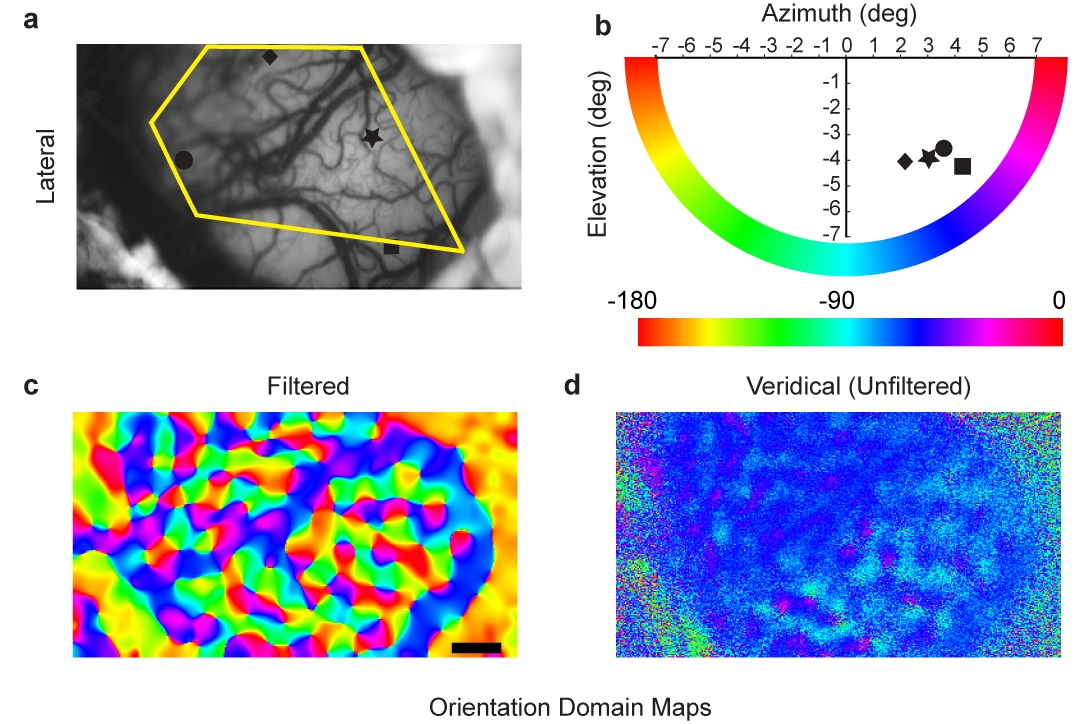
\includegraphics[width=\linewidth]{rb/figure1.jpg}
								\caption{Orientation tuning of the filtered and unfiltered signals. a) the cortical green image showing the cortical landmarks and the location of the electrode tracks. b) the different symbols indicate the receptive field location of the respective electrode tracks. The polar plot indicates the orientation of the unit obtained using single unit recording. The outer pseudo-color scale is the same as the one used in c and d. c) and d) are the filtered and the unfiltered maps.}
								\label{fig:rep}
							\end{figure}
			
			
			\begin{figure}[H]
				
				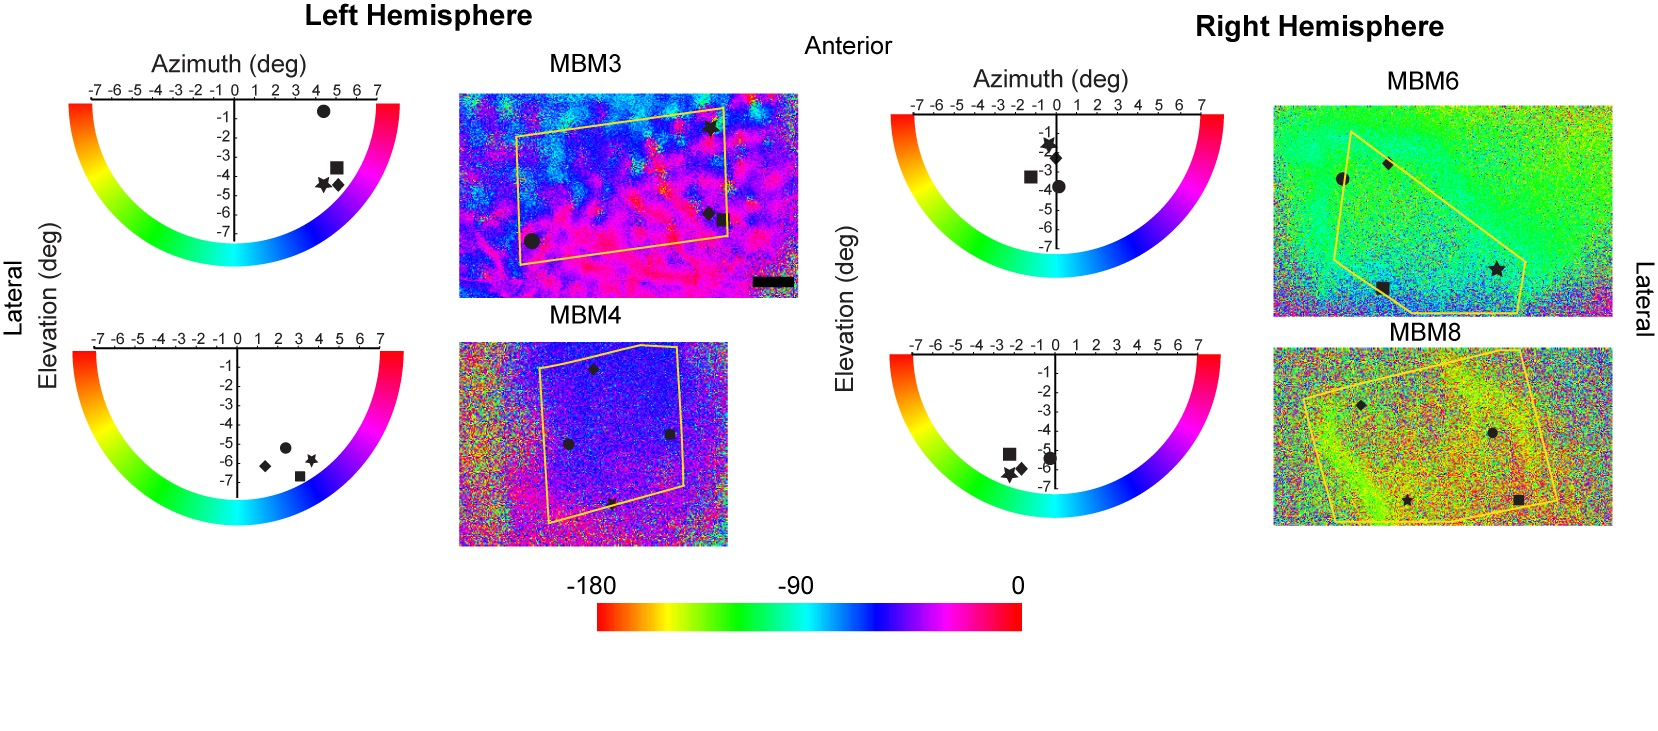
\includegraphics[width=\linewidth]{rb/figure2.jpg}
				\caption{The receptive field location, veridical and filtered orientation tuning maps of  all the animals (except that showed in figure \ref{fig:rep}) used in our studies. The conventions are as explained figure \ref{fig:rep}.}
				\label{fig:all}
			\end{figure}
							
		\subsubsection{Comparing the radial orientation and optimum orientation of ROIs}
		The optimum orientation of the pixels in the ROI and the radial angles of the ROIs were calculated and compared as described in the methods for 456 ROIs. Most ROIs were tuned to the radial orientation in the unfiltered maps. In the filtered maps, this bias for the radial orientation in the ROIs was observed to a smaller extent. Figure \ref{fig:roihist}a shows the distribution of the absolute differences between the optimum and radial orientations of the ROIs for the unfiltered and filtered orientation maps. The distribution of differences was significantly different from a uniform distribution for the unfiltered ($\chi^2$= 505.28; df=3; p$<$0.0001) as well as the filtered conditions ($\chi^2$= 35.21; df=3; p$<$0.0001). The filtered and the unfiltered distributions were also significantly different from each other ($\chi^2$= 283.01; df=3; p$<$0.0001).
			
			\begin{figure}[H]
				
				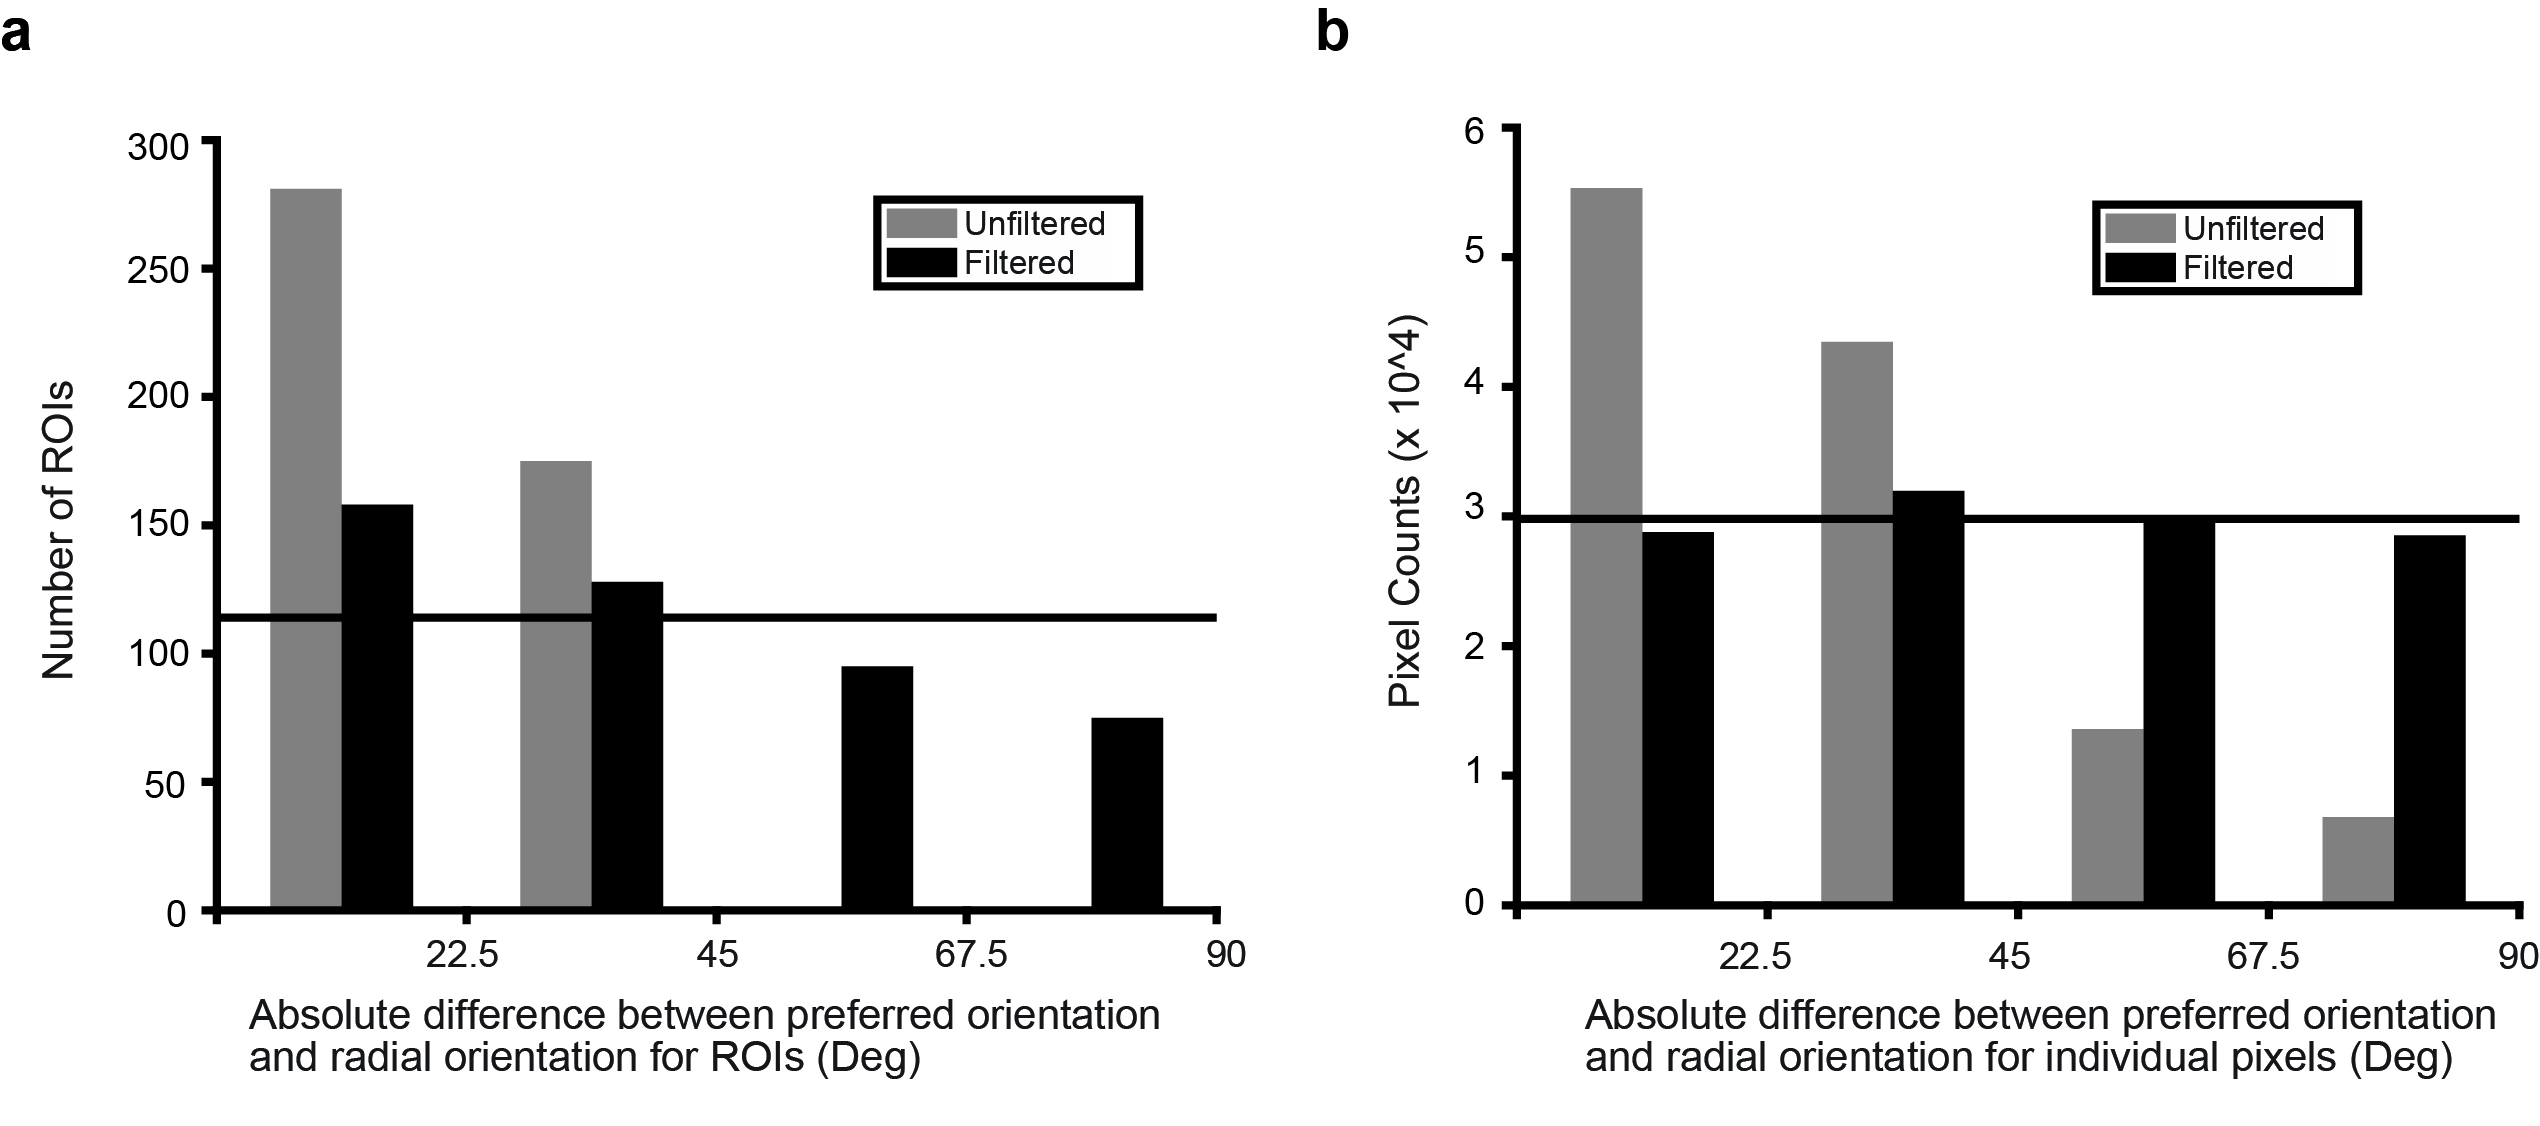
\includegraphics[width=\linewidth]{rb/FinalFigures/ROIhist.jpg}
				\caption{a) The absolute difference between the optimum orientation and the corresponding radial angle of the ROIs. Horizontal line is the distribution we would expect if the distribution was uniform. Total number of ROIs= 456. b) The distribution of absolute differences between the optimum orientation of single pixels and the radial angle of the imaged area.}
				\label{fig:roihist}
			\end{figure}
		\subsubsection{Comparing the radial orientation and optimum orientation of single pixels}
		The ROIs average the signal over 900 pixels (30X30 pixel square). We also examined the difference between the optimum orientation of individual pixels and the mean radial orientation of the imaged area to see if the radial bias was also present at the single pixel level. The single pixel differences showed that most pixels in the unfiltered condition were tuned to the radial orientation. Figure 6 shows the distribution of differences between the individual pixels and the mean radial orientation for the unfiltered and the filtered conditions. Once again, there was a strong peak between 0 and 22.5 degrees in the unfiltered condition. When compared with a uniform distribution (indicated by the horizontal line); the distribution of the differences for the unfiltered condition was significantly different (n= 119229; ($\chi^2$= 54691; df=3; p$<$0.0001). No clear anisotropies were observed in the filtered single pixel responses although the overall response was still significantly different from a uniform distribution (n= 119229; ($\chi^2$= 246.24; df=3; p$<$0.0001). The distribution of the filtered differences were also significantly different from the unfiltered differences (n=119229; ($\chi^2$= 54077; df=3; p$<$0.0001). We did not find any significant biases for horizontal and vertical orientations in either the ROI or the single pixel data.	
			
		For the single pixel analysis, as we used a large sample size (119229), the chi-square test, will always give a significant result regardless of the effect size. In order to address this issue, we used a repeated sampling paradigm, where smaller samples were randomly chosen from the overall pixel population and chi-square tests were performed on these distributions. We used two sample sizes (either 40 or 1000) and sampled 1000 times (1000 trials) from the overall population. The results indicate that the radial bias observed in the unfiltered maps were strong and were observed even in the condition with a relatively small sample size of 40 pixels (mean $\chi^2$= 21.09; CI= [20.95, 21.24];$\chi^2$ critical =7.05). There was also a statistically significant radial bias observed with the larger sample size of 1000 pixels for the unfiltered maps (mean $\chi^2$= 461.93; CI= [461.68, 462.19]; $\chi^2$ critical =7.05). For the filtered maps however, while the distribution was significantly different from a uniform distribution when sample size was 119229, the distribution was not significantly different from a uniform distribution when the sample size was 40 (mean $\chi^2$= 2.99; CI= [2.84, 3.13]; $\chi^2$ critical =7.05) or 1000 (mean $\chi^2$= 5.18; CI= [4.92, 5.44]; $\chi^2$ critical =7.05). These results suggest that the statistically significant result shown for a sample size of 119229 was most likely due to the large sample size. A summary of these results are presented in figures \ref{fig:s40} and \ref{fig:s1000} for the 40 and 1000 pixel samples respectively.
			
				
				\begin{figure}[H]
					
					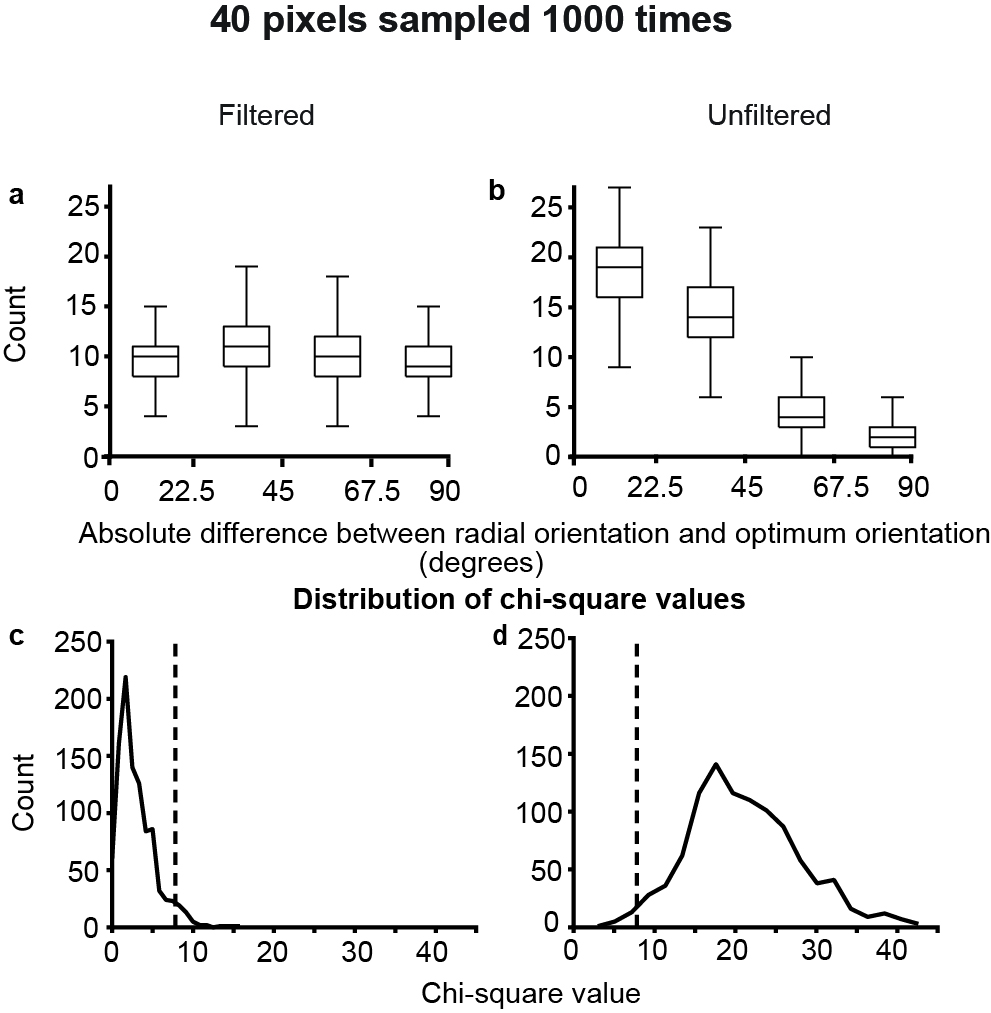
\includegraphics[width=\linewidth]{rb/FinalFigures/s3.jpg}
					\caption{Results of the random simulation experiment with 40 pixels sampled 1000 times. a) and b) show the distribution of the preferred orientation of the single pixels, centered on the radial orientation in the filtered and unfiltered conditions respectively. The boxplot indicates the distribution of the values over 1000 trials. c) and d) show the distribution of χ2 values for 1000 trials. The dotted lines indicate the location of the critical value for p=0.05.}
					\label{fig:s40}
				\end{figure}
				
				\begin{figure}[H]
					
					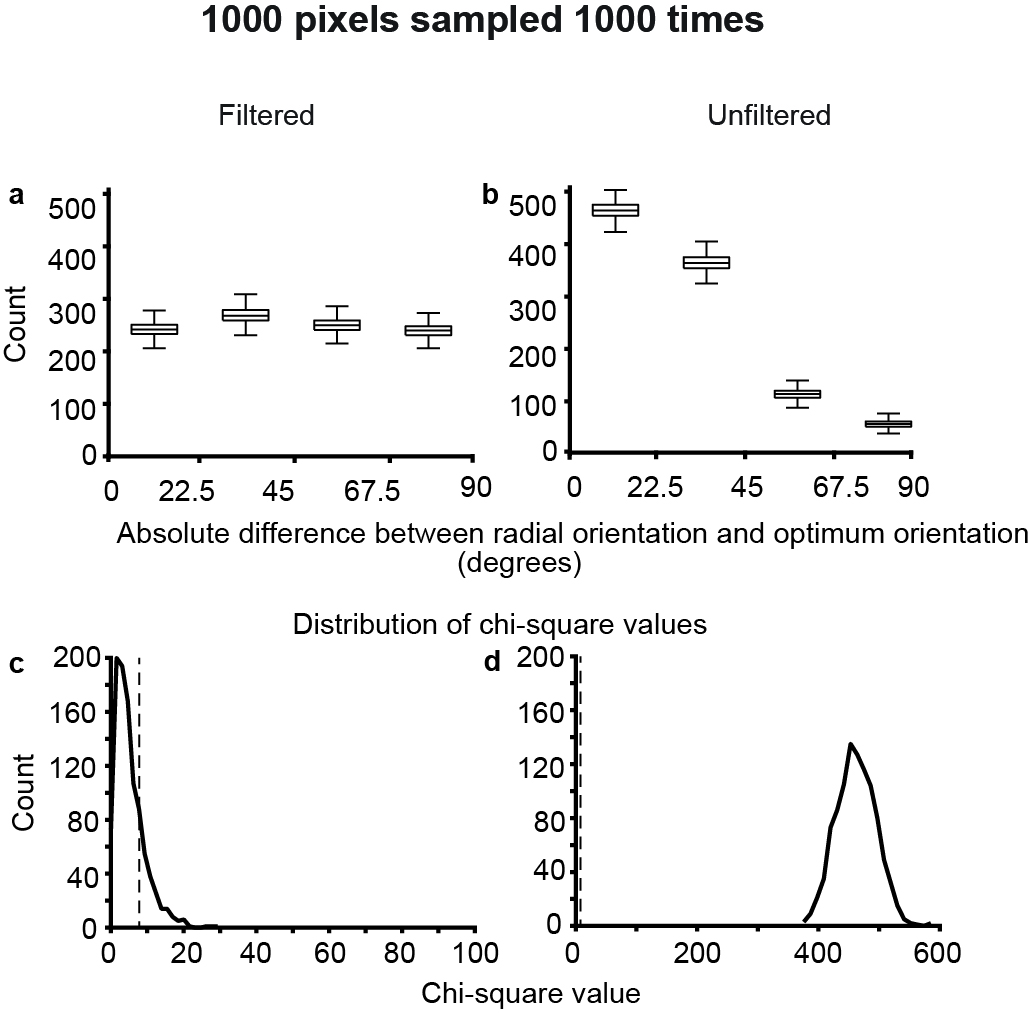
\includegraphics[width=\linewidth]{rb/FinalFigures/s4.jpg}
					\caption{Results of the random simulation experiment with 1000 pixels sampled 1000 times. See figure 6 for description of individual panels}
					\label{fig:s1000}
				\end{figure}
		\subsubsection{Orientation biases of the local field potentials}
		In two animals, we used single electrodes to record LFP as well as MUA from 6 recording sites. In one animal we used a multi-electrode array to record the LFP and MUA at a further 16 locations. The orientation tuning of the MUA and LFP of the array data are presented in figure 8. The multiunit activity changed consistently across subsequent electrodes so that most orientations were represented. The LFP activity on the other hand showed broader orientation tuning. Further, most sites were tuned to the radial orientation. The absolute differences between the optimum orientation of the LFP and the multiunit activity, and the radial angle of the imaged area are shown in figure \ref{fig:MUA} . This includes all 22 sites (from single electrodes and multi electrode arrays). A chi-squared test showed that the distribution of the differences of circular means of the LFP was significantly different from a uniform distribution (n=22;  $\chi^2$= 8.18; df=3; p=0.04) whereas the same was not true for the multi-unit activity (n=22;  $\chi^2$= 3.09; df=3; p=0.38).
				\begin{figure}[H]
					
					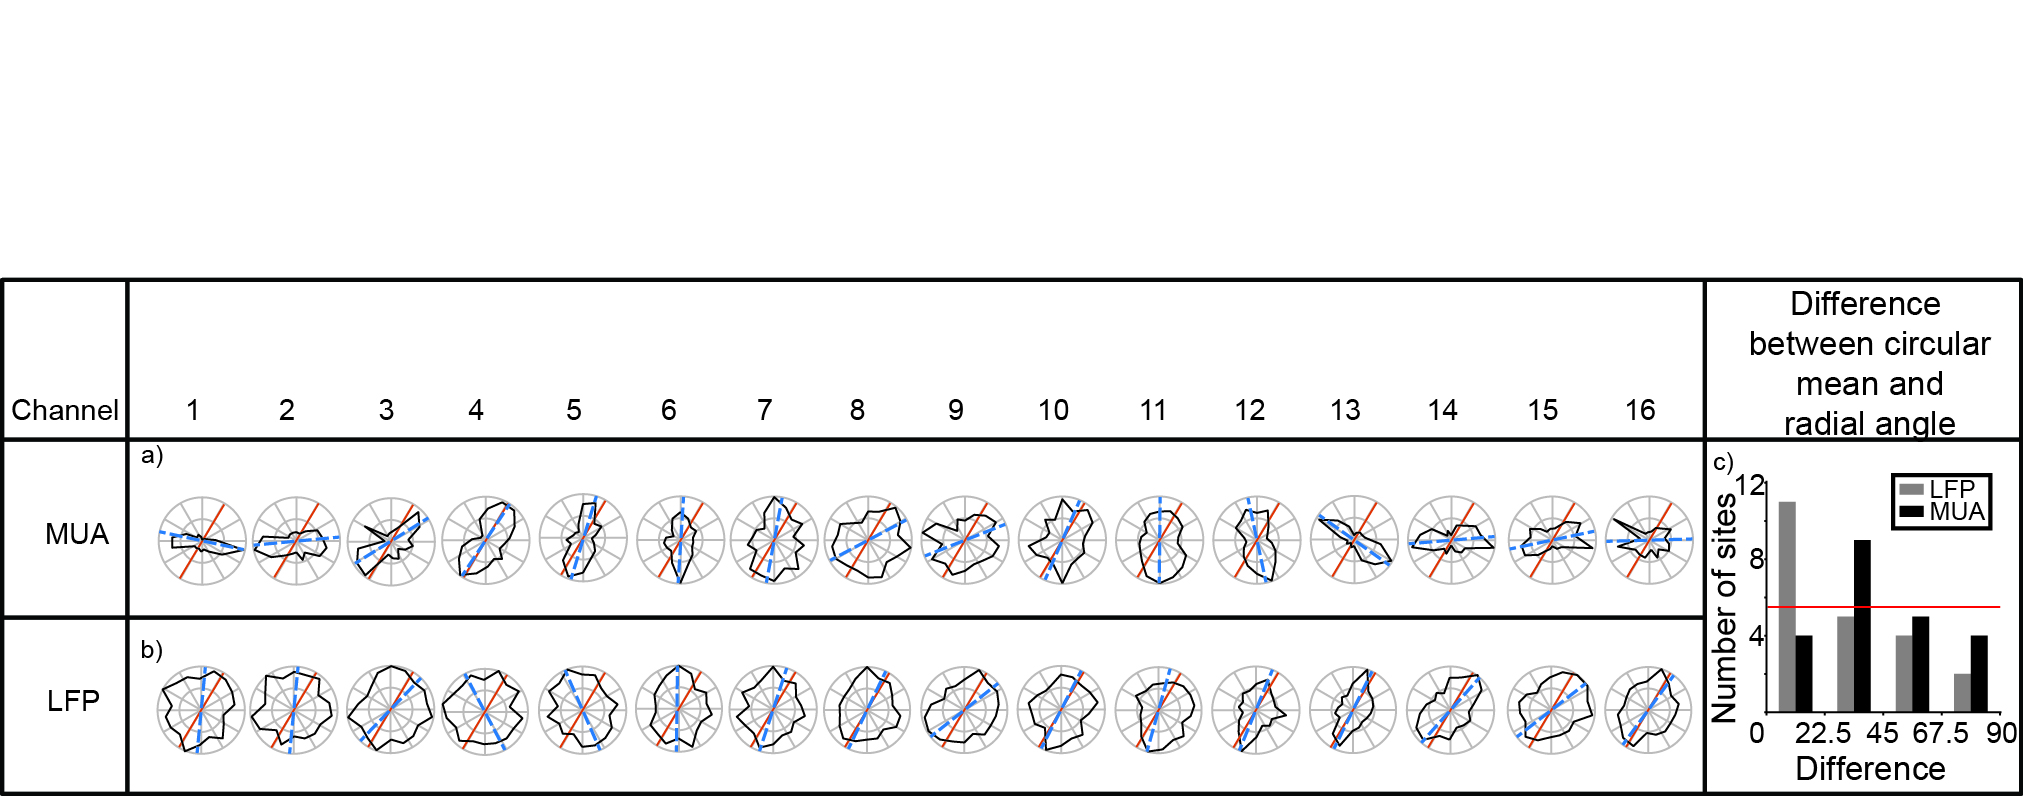
\includegraphics[width=\linewidth]{rb/FinalFigures/mua.jpg}
					\caption{Results of the random simulation experiment with 1000 pixels sampled 1000 times. See figure 6 for description of individual panels}
					\label{fig:MUA}
				\end{figure}
	
				\pagebreak
				
	\section{Discussion}
		
		Using optical imaging of intrinsic signals, we examined the OI signals at different spatial scales in the primary visual cortex of macaques. In a subset of animals, we also measured multi-unit responses and local field potentials in the primary visual cortex. We found that the large spatial scale signals in the OI and the LFP signals were tuned to the radial orientation while the smaller spatial scale signal and the multiunit responses did not show this preference for the radial angle. These results are consistent with the results from fMRI studies, where the BOLD signal is analogous to the OI haemodynamic signal, as well as the electrophysiological studies which show that in most animals studied, a radial bias exists in the visual system.
		
		During the experiment, we could have introduced systematic errors in various stages of data collection and analysis. The plotting of the foveal location is dependent on the visibility of the fovea when observed through the fundus camera. The visibility of the fovea itself is dependent on the optics which tend to deteriorate as the experiment progresses. During the experiment, we were able to more accurately characterise the optic nerve head. As a result, both the optic nerve and the first foveal position needed to be accurately plotted for us to accurately determine the radial angle. An error in plotting either of these parameters could lead to inaccurate estimation of the radial angle.
		
		Receptive field estimation is also subject to error. Within a track, there is a jitter of approximately half a degree in both receptive field position and size of the receptive field (Dow et al., 1981). Further, we also only used the receptive field position of the first unit encountered in each track. This was to make sure that the angle of the electrode to the surface did not affect the measurement of receptive field location. This compared with the fact that the ROI centres are extrapolated from the RF measurements could introduce another element of error in our radial angle estimates. The formula used for extrapolation, though standardised, may not be exactly accurate in every animal. Large variances in topography between individual animals (eg: See Dow et al., 1981) have been reported in macaques which could further compound the error in radial angle estimates.
		
		Further, the single pixel optimum orientations were all compared to the mean radial angle of the imaged area. The radial angles of the receptive fields in the imaged area can vary up to 30 degrees depending on the eccentricity of the receptive fields in the imaged area. This introduces a further element of error in the measurements which contribute to a larger spread of differences in the single pixel data. Taking into account all these sources of error in determining the difference between the radial angle and optimum orientation, the actual radial bias in the data may be stronger than has been reported.
		
		
		In our study, we have shown that the larger spatial scale activity is tuned to the radial orientation. However, the question of what these signals represent remains. The large spatial scale, global signal has been attributed to local blood flow and blood volume changes in the imaged area (Stetter et al., 2000; Pouratian and Toga, 2002). However, studies have shown that blood flow is also affected by neuronal activity through glial cells (Atwell et al., 2010), indicating that the blood volume changes accompany neuronal activity. One explanation lies in the fact that the BOLD responses (and therefore OI signals) are correlated with the LFP responses (Logothetis et al., 2001). This relationship is also demonstrated in our study, where the LFP and the ‘global’ OI signal were both predominantly tuned to the radial orientation. While the exact nature of the LFP signal is still not understood, general consensus is that this signal represents the synaptic, pre-synaptic and multi-unit observed in the recorded region of cortex and does not correspond well with the multi-unit activity (Berens et al., 2008; Logothetis et al., 2001). We propose that the larger spatial scale, global signal also corresponds with the pre-synaptic, synaptic and multi-unit activity. By removing the higher magnitude, larger spatial scale signals using a band-pass filter, optical imaging studies help isolate the responses that correspond to the scale of the multiunit activity. Therefore, the large spatial scale signal in the OI response corresponds to the synaptic and pre-synaptic activity, which reflect the tuning of the inputs to the imaged area. Our results indicate that the inputs to the primary visual cortex are tuned to the radial orientation.
	
		During imaging, the tandem lens arrangement allows us to focus on a very narrow plane under the surface of the cortex while imaging (Frostig et al.,1990). In this study, we focussed the tandem lens setup between 550-700 microns below the cortical surface. This depth corresponds to the region of the cortex just above the interface between Layer 3 and Layer 4. Unlike the cat Area 17, most neurons in the macaque layer 4 show broad orientation tuning, with sharp orientation emerging in Layers 2 and 3 for the first time (Bullier and Henry, 1980). Further, the areas of layers 2 and 3 that were imaged also receive direct inputs from konio-cellular layers of the LGN (Klein et al., 2016). This indicates that the cells in the imaged layer, like their layer 4 counterparts show broad orientation selectivity. Therefore, despite the depth where the camera was focussed and images were obtained from, we can conclude that the inputs to the cortex are tuned to the radial orientation.
	
		A previous study from our lab showed that inputs to neurons in the primary visual cortex were tuned to the same orientation as the orientation column to which they project (Vidyasagar et al., 2015). These results are not entirely contradictory to the results from our current study. Apart from any species differences that may be present, the earlier study showed a considerable jitter in the relationship between the orientation of the LGN fibres and cortical columns (r= 0.63). In our study, while the majority of the ROIs and pixels  in the unfiltered maps were tuned to the radial angle, there were also a proportion that were tuned betweem 22.5 and 90 degrees away from the radial angle. This departure from the radial angle is similar to that shown in the earlier study (Vidyasagar et al., 2015). 
		
		If the inputs to the primary visual cortex are tuned to the radial orientation, then this has some implications for orientation selectivity in the primary visual cortex. The theory of excitatory convergence for the generation of orientation selectivity was first proposed by Hubel and Wiesel (1962) and proposed that thalamic neurons with circular receptive fields arranged in a row converged on a striate cortical neuron to endow on it sharp orientation selectivity. This model assumption that thalamic neurons are untuned to orientation. Contrary to this belief, many studies have shown that subcortical neurons are indeed biased for orientation (Hammond, 1974; Levick and Thibos, 1980; Vidyasagar and Urbas, 1982; Leventhal, 1983; Van Hooser et al., 2013Vidyasagar and Henry, 1990; Smith et al., 1990; Passaglia et al., 2003; Shou and Leventhal, 1989; Sun et al., 2016). Our study adds to this extensive literature on sub-cortical biases by studying the organisation of the orientation selectivity of the inputs in the cortex, suggesting that most of these inputs are tuned to just one orientation. This provides support for a model of orientation selectivity where the inputs to the cortex arrive in a small number of broadly tuned orientation channels, from which the whole range of orientations observed in the primary visual cortex are generated (Vidyasagar and Eysel, 2015).
		
		Vidyasagar and Eysel (2015) proposed that all orientations in the cortex can be generated by broadly tuned orientation channels with orthogonal orientations. However, our study only shows a bias for the radial angle in the inputs to the cortex. orientations. This does not necessarily mean that only one orientation is present in the inputs. The large magnitude of the radial bias signal could mean that any smaller signals maybe masked. There are no ways to separate these signals on a spatially (as is usually done in the case of extracellular signals) without losing the information. Even if only one clear bias is present in the inputs, the cortex may still be able to generate all orientations. For example, phase selectivity is completely dominated by one polarity (75\% of neurons respond to light off; Albus and Wolf, 1984) in kittens but the cortical networks generates both on and off neurons from these limited inputs (Xin et al., 2008). In colour vision too, normal colour vision can be achieved even though there are only a relatively small proportion of S cones and large variation in the proportion of L and M cones (Kremers et al., 2000).
	
		Our study also highlights the importance of studying the optical imaging signal at different spatial scales as has been previously shown in cats, humans and macaques (Swisher et al., 2010; Tanigawa et al., 2017). In this study, we also highlight the use of optical imaging of intrinsic signals in studying the organisation of cortical inputs on a larger spatial scale. Future study can further characterise this large spatial scale, global signal which may be useful in determining organisation of inputs to the cortex.
		\pagebreak
	\section{Conclusion}
	
		In this chapter, we aimed to examine the large spatial scale activity in orientation maps to characterise radial bias in the optical imaging signal. We compared the optimum orientations of single pixels and ROIs to their radial angles and found that in the unfiltered maps, there was a prominent bias for the radial angle. The ROIs in the filtered maps showed a weaker bias for the radial orientation but no such bias was observed in the single pixel responses. We propose that these signals reflect the orientation tuning of the inputs to the cortex. If the majority of the inputs to the cortex are indeed tuned to the radial angle, then this provides evidence for a model of orientation selectivity where orientation input arriving in a small number of broadly tuned channel are further sharpened in the primary visual cortex to generate the whole range of orientation preferences observed in the cortex. 
		
	
\chapter{Mechanism of orientation selectivity in the tree shrew primary visual cortex}


\section{Summary}


\section{Introduction}

The tree shrew is a highly visual mammal that is closely related to
primates. While in the cat visual system, sharp orientation selectivity
is already present in layer 4 of the primary visual cortex, in macaques
and tree shrews, this transformation occurs from layer 4 to layer 2/3.
Similarly, where in the cats, LGN neurons are low pass tuned for spatial
frequency, layer 4 neurons show band-pass spatial frequency tuning, in
the tree shrews this transformation occurs from layer 4 to layer 2/3 in
V1. In this chapter, we examined if the orientation selectivity of the
tree shrew layer 2/3 neurons arise from a similar mechanism as has been
described in cats and macaques. As the sharpening of feature selectivity
occurs entirely within V1, experimenting in tree shrews gives us the
opportunity to examine the mechanism through which receptive field
properties are generated within a single electrode track rather than
paired recordings from more than one visual area. This also gives us the
added advantage of recording from neurons that are matched for
eccentricity, as this is an important caveat while comparing spatial
frequency tuning from different visual areas.

In the tree shrew, orientation selectivity in layer 2/3 neurons was
initially thought to have originated from excitatory convergence of a
number of layer 4 neurons arranged in a row (Mooser et al., 2004) as has
been proposed in cats and macaques (Hubel \& Wiesel, 1962; 1968).
However, when the data was carefully examined, it was found that the
elongation of the receptive fields in shrew layer 2/3 was much smaller
than would have been expected from a purely feed-forward mechanism. As a
result, it was proposed that the prominent horizontal connections
present in layer 2/3 further sharpened the orientation selectivity of
neurons (Bosking et al., 1997; Chisum et al., 2003; Mooser et al., 2004;
Veit et al., 2013). One study that used optogenetics and optical imaging
of intrinsic signals however showed that horizontal connections in the
layer 2/3 of tree shrew V1 did not have a modulatory effect on the
neuronal responses as previously suggested but rather had an additive
effect (Huang et al., 2014). Recently, Lee et al. (2016), suggested that
the orientation selectivity in the shrew V1 was established by the
spatially off on and off inputs as has been proposed in the cats (Soodak
\ldots{}Kremkow et al., 2016). However, Muly and Fitzpatrick (1992)
showed that on and off inputs to layer 2/3 cells have significant
overlap, preventing extensive segregation of sub-regions in tree shrews.
As a result, the mechanism through which orientation tuning comes about
in the shrew V1 is as yet unclear.

It is possible that orientation selectivity in the tree shrews can arise
from the anisotropic LGN Driven-Recurrent Model (ALD-RM; Vidyasagar et
al., 1996; Kuhlmann \& Vidyasagar, 2011; see Figure 1). In the cortex,
most cortical neurons receive direct excitatory inputs from sub-cortical
neurons biased for orientation and di-synaptic input from un-oriented
sub-cortical neurons via inhibitory interneurons (Creutzfeldt \& Ito,
1968; Ferster \& Lindstrom, 1983). The inhibitory input increases the
threshold for firing in the cortical neuron and the remaining signal
would automatically be tuned for orientation. Orientation selectivity
could then be further sharpened by intracortical mechanisms such as
recurrent excitation (Ref) and cross-orientation inhibition (ref). The
ALD-RM model also explained the spatial frequency tuning of neurons in
both the LGN as well as the layer 4 neurons in cats. LGN neurons showed
low-pass spatial frequency tuning (Ref) and at these spatial
frequencies, they fire well to all orientations (Vidyasagar \& Heide,
1984). At higher spatial frequencies however, the neurons show
orientation selectivity. Cortical neurons show band-pass spatial
frequency tuning and fire only at spatial frequencies where the LGN
neurons are tuned to orientation (Ref). The di-synaptic inhibition in
cortical neurons will be non-specific to orientation at lower spatial
frequencies where the LGN neuron is not tuned to orientation and causes
general attenuation at these lower spatial frequencies. At higher
spatial frequencies, the signal that remains is sharply tuned to both
the orientation and spatial frequency. The receptive fields of the
neurons in such a scheme in cat is shown in figure 1b.

\begin{figure}[H]
	\centering
	\includegraphics[width=0.8\linewidth]{ShrewV1/orituning_scheme.jpg}
	
	\caption{Mechanism of orientation selectivity proposed in cats and tree
		shrews. In the cats, layer 4 neurons receive excitatory input from an
		LGN neuron biased for the same orientation and di-synaptic input via an
		inhibitory neuron from an LGN neurons unbiased for orientation. The
		orientation non-specific inhibitory input increases the threshold of
		firing from the cortical neuron and the resulting signal is tuned for
		orientation. A similar transformation occurred from layer 4 to layer 2/3
		in the tree shrews.}
	\label{fig:orischeme}
\end{figure}



In figure 1b, the excitatory and inhibitory inputs to a layer 2/3 neuron
in the tree shrew cortex are shown. Each layer 2/3 neuron in the tree
shrew V1 receives converging excitatory inputs from on and off layer 4
neurons (Muly \& Fitzpatrick, 1992) and has extensive horizontal
connections (Bosking et al., 1997). Layer 4 neurons are also broadly
tuned to orientation and show low pass spatial frequency tuning while
layer 2/3 neurons show sharp orientation selectivity and show band-pass
spatial frequency tuning (Van Hooser et al., 2013). It could be that a
similar transformation that occurs from LGN to layer 4 in the cat visual
system happens from layer 4 to layer 2/3 in the tree shrews. We tested
the following hypothesis to test whether this was indeed the case.

\textbf{(H1)} As neurons in the on and off sub-divisions of layer 4
converge onto layer 2/3 neurons directly above them and most layer 4
neurons demonstrate orientation biases, we predicted that most of the
layer 4 and layer 2/3 neurons in the same track were tuned to the same
orientation.

\textbf{(H2)} Orientation tuning of layer 4 neurons are evident at
higher spatial frequencies similar to that of cat LGN neurons.

\textbf{(H3)} Finally, we predicted that layer 2/3 neurons fire best at
spatial frequencies where the layer 4 neuron is best tuned for
orientation.


\section{Methods}


\subsubsection{Surgery and Anaesthesia}

Detailed surgical procedures are outlined in the Methods chapter.
Briefly, the animal was anaesthetized using a mixture of Ketamine and
Xylazine, a venous catheter was inserted in to the femoral vein and a
tracheostomy performed to assist in breathing during the experiment. The
animal was administered muscle paralysant (Vecuronium Bromide)
intravenously and was anaesthetised using Isoflurane (0.5-1\%) for the
duration of the experiment. Hard contact lenses were fitted to the eye
to prevent corneal drying. In some tree shrews, additional lenses were
used to correct for any refractive errors. A craniotomy and durotomy
were performed over the location of V1 (Horsley-Clarke Co-ordinates A2.5
to P2.5). ECG and frontal EEG were monitored during the experiment. At
the end of the experiment, the animal was euthanized using an overdose
of pentobarbital sodium and perfused using 0.1M Phosphate Buffer (PB)
solution followed by 4\% Paraformaldehyde in 0.1M PB. The brain was
removed and stored in sucrose (20-25\%) for histology.


\subsubsection{Electrophysiology}

High impedence, lacquer coated tungsten microelectrodes (FHC Metal
Microelectrodes Inc., ME, USA; impedance= 12-18 MΩ) were lowered into
the brain at an angle perpendicular to the cortical surface. The signal
was amplified and filtered (x 10,000 gain, bandpass filtered between
300-3000 Hz, A-M systems) and fed into an audio speaker as well as an
analog to digital converter (Cambridge Electronic Design Limited,
Cambridge, UK; digitised at 22.5 kHz). Neurons were recorded from Layers
2/3 and Layer 4. Layer 4 could be identified by a characteristic
`swish', first for on stimuli and then for off stimuli, in the tree
shrews. Where we no longer heard the swish, we concluded that we exited
layer 4 and into layer 5. Neurons in layers 5 and 6 were not recorded
from. Lesions (6 μA for 6s) were made at the end of each track. The
electrode was withdrawn and lesions were made at regular intervals to
trace the path of the electrode through the brain. The data was recorded
as a spike trace using the spike 2 software (CED, Cambridge, UK). The
spikes were templated and the spike timing exported as a text file.
Further analysis was performed using custom MATLAB® code (The Mathworks
Inc, USA).


\subsubsection{Stimulus Presentation}

A hand-held projectoscope was used to mark the receptive field
boundaries. Using this, the centre of the monitor was aligned with
centre of the receptive field prior to stimulus presentation. Stimuli
were presented using a BARCO monitor (Frame Refresh Rate= 80 Hz;
Reference Calibrator Plus; Barco Video and Communications, Belgium) and
generated using Visage (VSG, Cambridge Research Systems, Cambridge, UK)
and custom Stimulus Description Language (SDL) scripts. While recording,
the monitor was placed at a distance of 114 cm from the eye. For each of
the different stimuli described below, ten complete stimulus sets were
completed.


\paragraph{Bar Stimuli}

For each neuron, an initial estimate of optimum orientation was obtained
using bars moving bi-directionally across the screen. The background was
a uniform gray screen. Depending on the polarity of the neurons, either
a light bar or a dark bar was used (contrast= 100 \%). The bar was
usually 8\textsuperscript{o} long (ranging between 4 and 8 degrees) and
0.5\textsuperscript{o} wide (ranging between 0.1 and
1\textsuperscript{o}). A total of 18 different orientations were tested
and PSTHs (see chapter 2) were made online using the Spike 2 software.
The orientation that yielded the highest firing rate was used for
further testing.


\paragraph{Grating Stimuli}

For all neurons, once optimum orientation was determined, spatial
frequency tuning was studied. Drifting sine-wave gratings (TF= 4Hz,
Contrast=100\%) of increasing spatial frequencies (between 0 and 2.2
cpd) and in the optimum orientation were presented to neurons. For layer
4 neurons, the spatial frequency response to gratings of the non-optimum
was also recorded. The responses were recorded and stored for further
analysis.

\paragraph{Data Analysis}

\subparagraph{Orientation Selectivity of bars}

The orientation selectivity of all the cortical neurons we encountered
were measured using thin bars. The circular mean and circular variance
of this response was calculated using the following formulas to measure
the optimum orientation and sharpness of the tuning.

\[CV = 1 - |\frac{mean(r*e^{(i*2\theta)})}{mean(r)}|\]

where \(\theta\) is the orientation of the bar and r is the response of
the bar to each orientation.

\[CM = atan(\frac{1}{n}.\sum_{j = 1}^{n}r*sin\theta,\frac{1}{n}.\sum_{j = 1}^{n}r*cos\theta)\]

One of the key predictions of our model was that the optimum orientation
of the neuronal responses did not vary along a penetration perpendicular
to the cortical surface. In order to test this hypothesis, we calculated
the absolute difference in preferred orientation between the first
neurons we encountered in layer 2/3 in each track and all the neurons
that were present in the same track.

It is possible that in our penetrations, the electrode angles were not
always exactly perpendicular to the cortical surface. In order to make
sure that any differences we observed in the optimum orientation were
not due to the angle of the track, we also undertook a simulation
experiment. We obtained an orientation tuning map of the tree shrew V1
(Bosking et al., 1997) and converted the RGB map into HSV co-ordinates.
We then converted the hue values into angles and used this map for
further analysis. A point was placed on the orientation map and the
orientation of a thousand pixels randomly placed at a particular
distance were subtracted from the orientation of the original pixel.
This procedure was repeated a 1000 times and for 6 distances (50, 100,
150, 200, 250, 300 mm). A probability histogram was calculated to
determine the probability of obtaining various absolute differences.


\subparagraph{Spatial Frequency Tuning}

For each layer 2/3 and layer 4 neuron, the spatial frequency tuning
curve was obtained from the response of the neuron to drifting gratings
of the optimum orientation and increasing spatial frequencies. The SDFs
(see Chapter 3: Methods) of the neuron were analysed using Fourier
Analysis (using the fast fourier transform algorithm (FFT) in MATLAB ®)
and a modified version of the F1/F0 ration called the modulation index
(as described by Van Hooser et al.,2013) was calculated using the
following formula.

\[Modulation\ Index(MI) = 2*\frac{F_{1}}{F_{1} + F_{0}}\]

If the MI was greater than 1, the neuron was classified as simple and
the F1 component was used as the response and if the MI was lesser than
1, the neuron was classified as complex and the DC component was used as
response. This version of the formula was used so that we could compare
our data to previously published data from the tree shrews. The upper
and lower cutoff frequencies were calculated as the frequencies above
and below the optimum spatial frequency where the response first dropped
below half the maximum response respectively. The bandwidth of the
neurons in octaves was calculated as follows.

\[b_{\text{oct}} = log2(\frac{\text{uppercutoff}}{\text{lowercutoff}})\]


\subparagraph{Orientation Tuning using Gratings}

For layer 4 neurons, the spatial frequency tuning of the neuron at the
optimum and the orthogonal orientations was also recorded. In our second
hypothesis (H2), we predicted that the orientation selectivity of layer
4 neurons would sharpen as the spatial frequency increased. We
calculated the orientation selectivity index (OSI) to determine the
orientation of the neurons at each spatial frequency as follows.

\[OSI = 1 - \frac{R_{\text{orthogonal}}}{R_{\text{optimum}}}\]

where R$_{orthogonal}$ is the response at the orthogonal
orientation and R$_{optimum}$ is the response at the optimum
orientation at each spatial frequency. Higher values of OSI mean that
the neuron showed sharper orientation tuning. The spatial frequency at
which the neuron showed maximum orientation selectivity was obtained.


\paragraph{Histology and Track Reconstruction}

At the end of each track an electrolytic lesion (6\(\mu\)a for 6s) was
made. After the experiment was completed, the brain was removed
following perfusion using 0.1M Phosphate Buffer and 4\% Paraformaldehyde
and was stained for Nissl substance using Cresyl Violet Acetate
(ph=3.4-3.6). The tracks were later reconstructed and the laminar
position of each neuron was determined.


\subsection{Results}


\subsubsection{Laminar Position of neurons}

We recorded from 75 neurons from the V1 of 13 tree shrews (M=6; F=7).
The laminar position of all units were determined using track
reconstructions based on lesions made during recording (yellow arrows in
fig 1a). In the tree shrew, the V1 shows prominent striation
corresponding to layer 4. Layer 3c is a cell sparse region just above
layer 4. Neurons recorded above layer 3c were classified as belonging to
layer 2/3. We recorded from 30 layer 2/3 neurons; 29 layer 4 neurons and
16 layer 3c neurons.

\begin{figure}[H]
	
	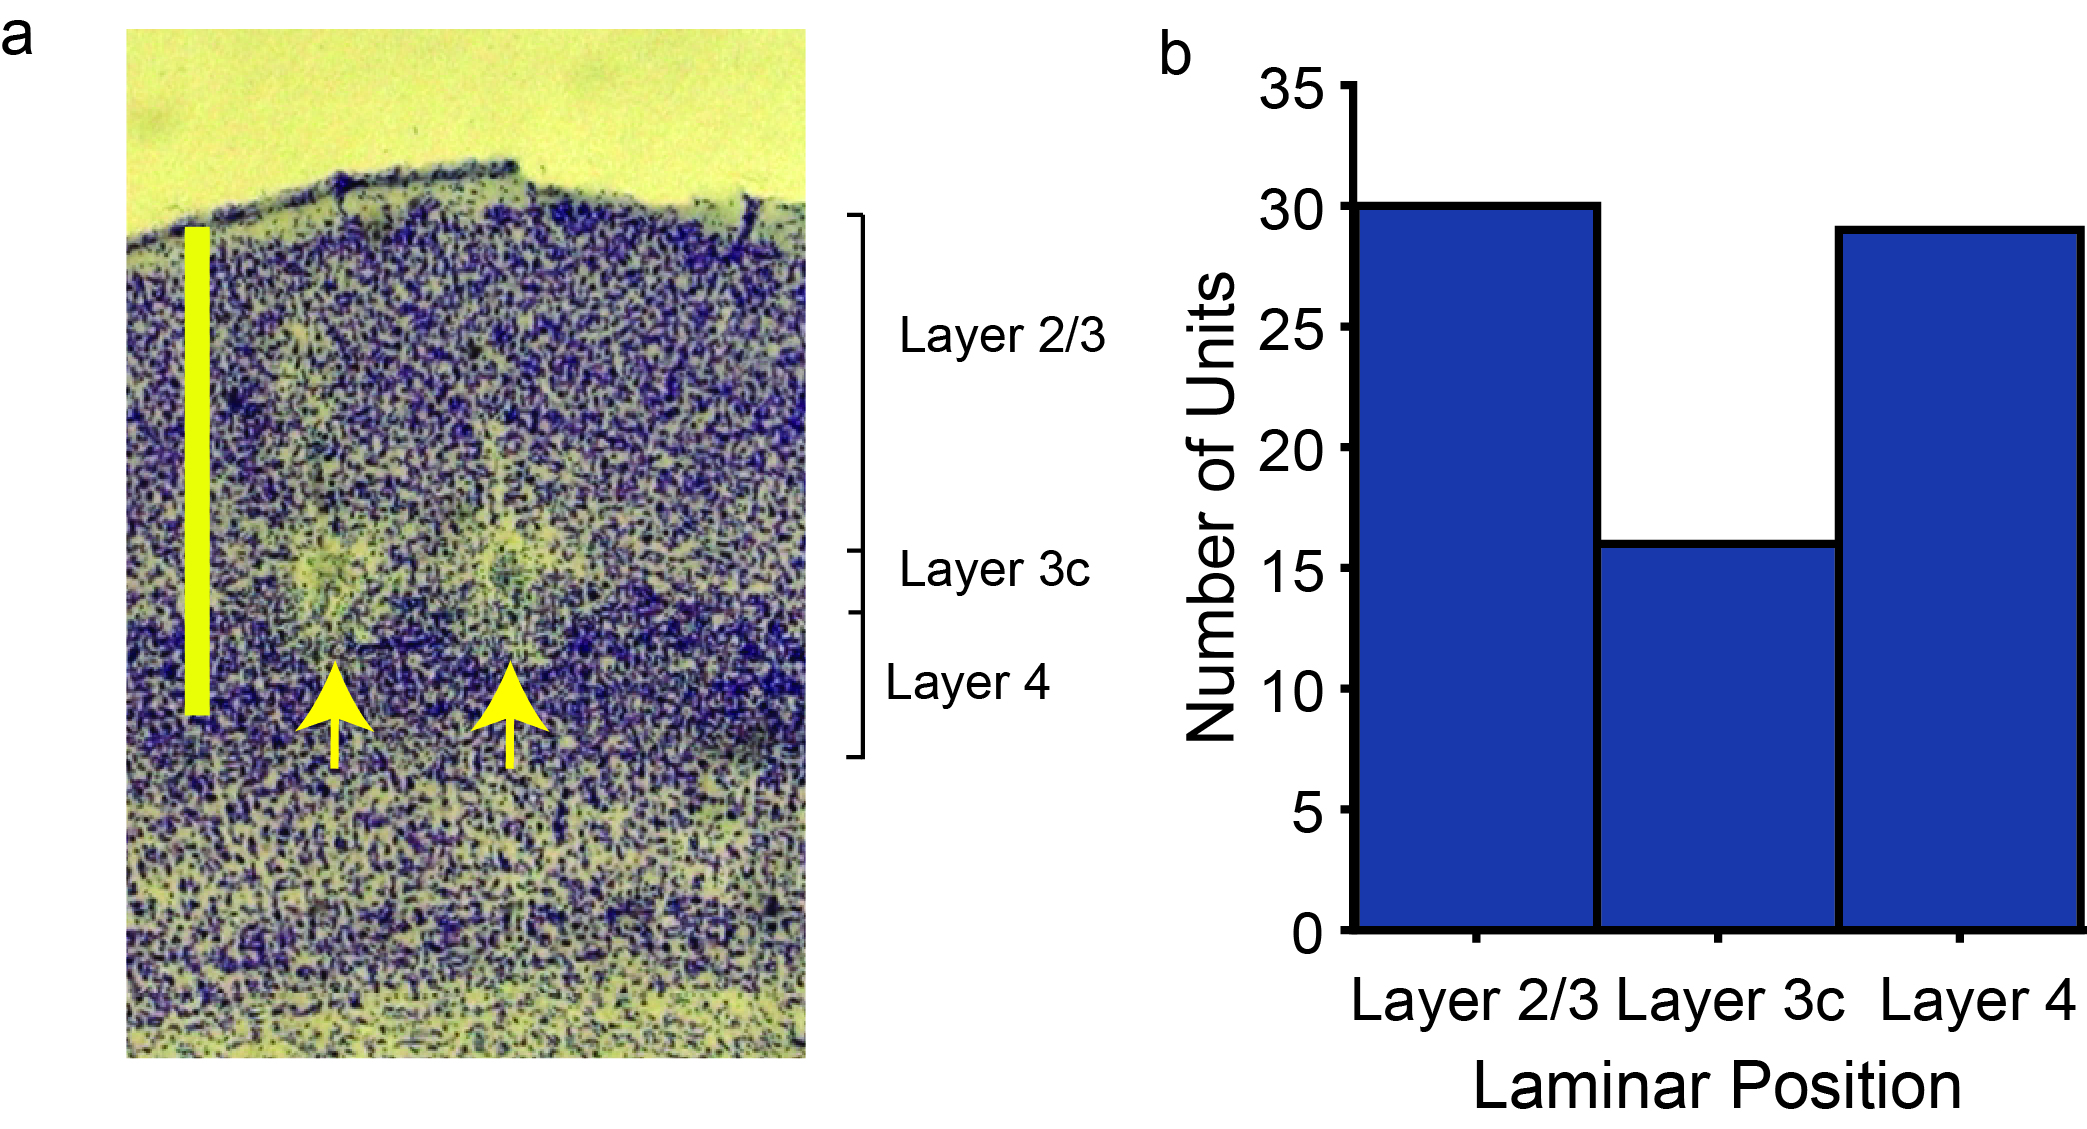
\includegraphics[width=\linewidth]{ShrewV1/LaminarPosition.jpg}
	\caption{The distribution of laminar positions from which we recorded. a) A photomicrograph of the tree shrew primary visual cortex with layers 2/3, 3c and 4 marked. The two arrows point to two lesions made in layer 3c of two separate tracks. The scale bar is 1 mm. b) Histogram showing the number of neurons recorded from each of the layers.}
	\label{fig:lp}
\end{figure} 


\subsubsection{Distribution of the circular variance}

The distribution of circular variances for neurons in the three layers,
calculated from their responses to thin moving bars are shown in fig 2.
The median CV of layer 2/3 neurons was 0.59 (n=28; 95\% CI= {[}0.32,
0.68{]}); that of layer 3c was 0.87 (n= 16; 95\% CI= {[}0.68, 0.91{]})
and that of layer 4 neurons was 0.88 (n=29; 95\% CI={[}0.84, 0.90 {]}).
The three distributions were significantly different from each other
(p\(<\)0.001, Kruskal-Wallis test). Post-hoc tests revealed that there
was a statistically significant distribution between the distribution of
CVs of neurons in layer 2/3 and layer 3c (Wilcoxon rank sum test,
z=2.37; p\(<\)0.01) and between layer 2/3 and layer 4 (Wilcoxon rank sum
test test, z= 3.58, p\(<\)0.001). The difference between the
distributions of CV of layer 3c neurons and layer 4 neurons was not
statistically significant (Wilcoxon rank sum test, z= 0.67; p=0.25).

\begin{figure}[H]
	
	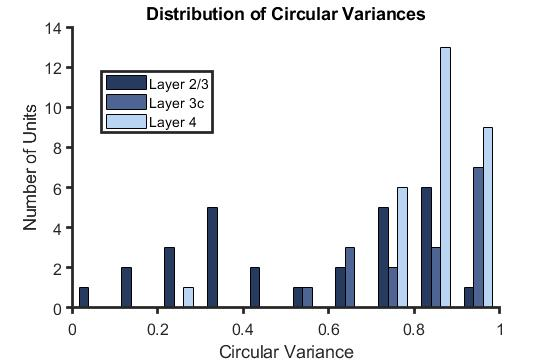
\includegraphics[width=\linewidth]{ShrewV1/cv_lamina_2_bw.jpg}
	\caption{The distribution of circular variance of neurons of the shrew V1.}
	\label{fig:cv}
\end{figure} 

\subsubsection{Circular mean of neurons}

In \textbf{{[}H1{]}}, we predicted that the layer 2/3 and layer 4
neurons in each track will have the same orientation. In this section,
we aimed to test this hypothesis. To test this hypothesis, we took the
absolute difference between the circular means of each layer 2/3 neuron
and all the layer 4 neurons from that track. Since layer 3c neurons
showed a similar degree of orientation selectivity as the layer 4
neurons and it has been shown that layer 3c also receive direct inputs
from the LGN (Reference), we also took the absolute difference of the
layer 3c neuron's orientation from the corresponding layer 2/3 neuron.
The results from 37 pairs of neurons from 18 tracks are presented in fig
3. We found that there were two peaks, one with the centre at
0\textsuperscript{o} and the other at 65\textsuperscript{o}. The
distribution of absolute differences was significantly different from a
uniform distribution (chi-square test; n=37; df=5; chi-square=12.35;
p\textless{}0.005).

	\begin{figure}[H]
	\centering
	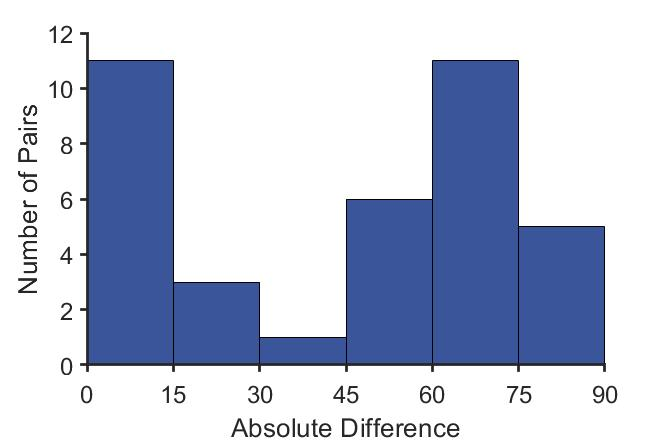
\includegraphics[width=0.5\linewidth]{ShrewV1/cmdiff.jpg}
	\caption{The absolute difference between the circular mean of the first layer 2/3 neurons in each track and subsequent neurons from layer 3c and layer 4 in each track.}
	\label{fig:cmdiff}
\end{figure}


We then split the distribution into two groups: pairs of neurons that
were tuned to orientations less than 45\textsuperscript{o} (Group 1)
apart and pairs tuned to orientation greater than 45\textsuperscript{o}
apart (Group 2). We then determined if the absolute difference was
between the layer 2/3 neuron and layer 3c neurons or between layer 2/3
neuron and layer 4 neurons. These results are shown in fig.4. We found
that in Group 1, the majority of the difference pairs were between layer
2/3 and layer 4 neurons (N=15; Binomial Distribution, p=0.04). In Group
2, majority of the difference pairs were between layer 2/3 and layer 3c
neurons (N=22; Binomial Distribution, p=0.04)


\begin{figure}[H]
	\centering
	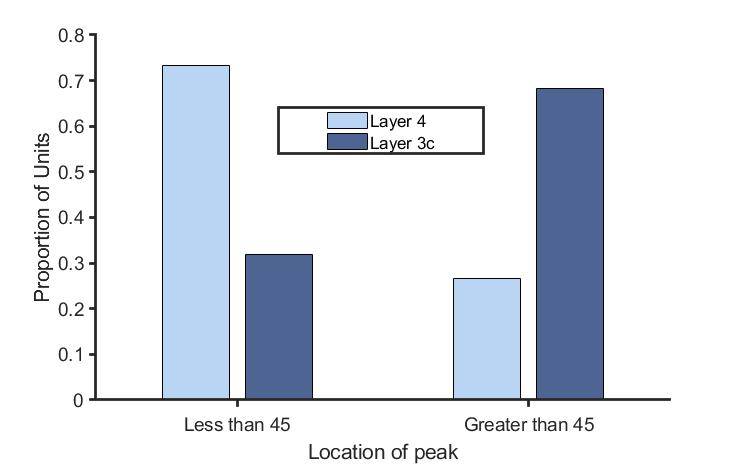
\includegraphics[width= 0.5\linewidth]{ShrewV1/cmlayer.jpg}
	\caption{The proportion of neurons from layers 3c and layer 4 with absolute differences greater and lesser than 45$^o$.}
	\label{fig:cmlayer}
\end{figure}

In order to ensure that the second peak we observed in fig. 4 wasn't due
to track angles, we undertook a simulation experiment (See methods
section). We found that for the shortest distance between the layer 2/3
and layer 4 neurons in our sample (50 mm), there was a high probability
of getting an absolute difference of 0 but this probability decreased
steadily. For the greatest horizontal distance between two neurons in
our sample (300 mm), the probability of obtaining the same orientation
was lower. While there was a general trend towards getting neurons that
were tuned closer to 90\textsuperscript{o} apart, there was no specific
bias for a difference of 65\textsuperscript{o}. The highest probability
of obtaining a peak at 65\textsuperscript{o} was when the horizontal
distance was 250 mm (p=0.045).

\begin{figure}[H]
	\centering
	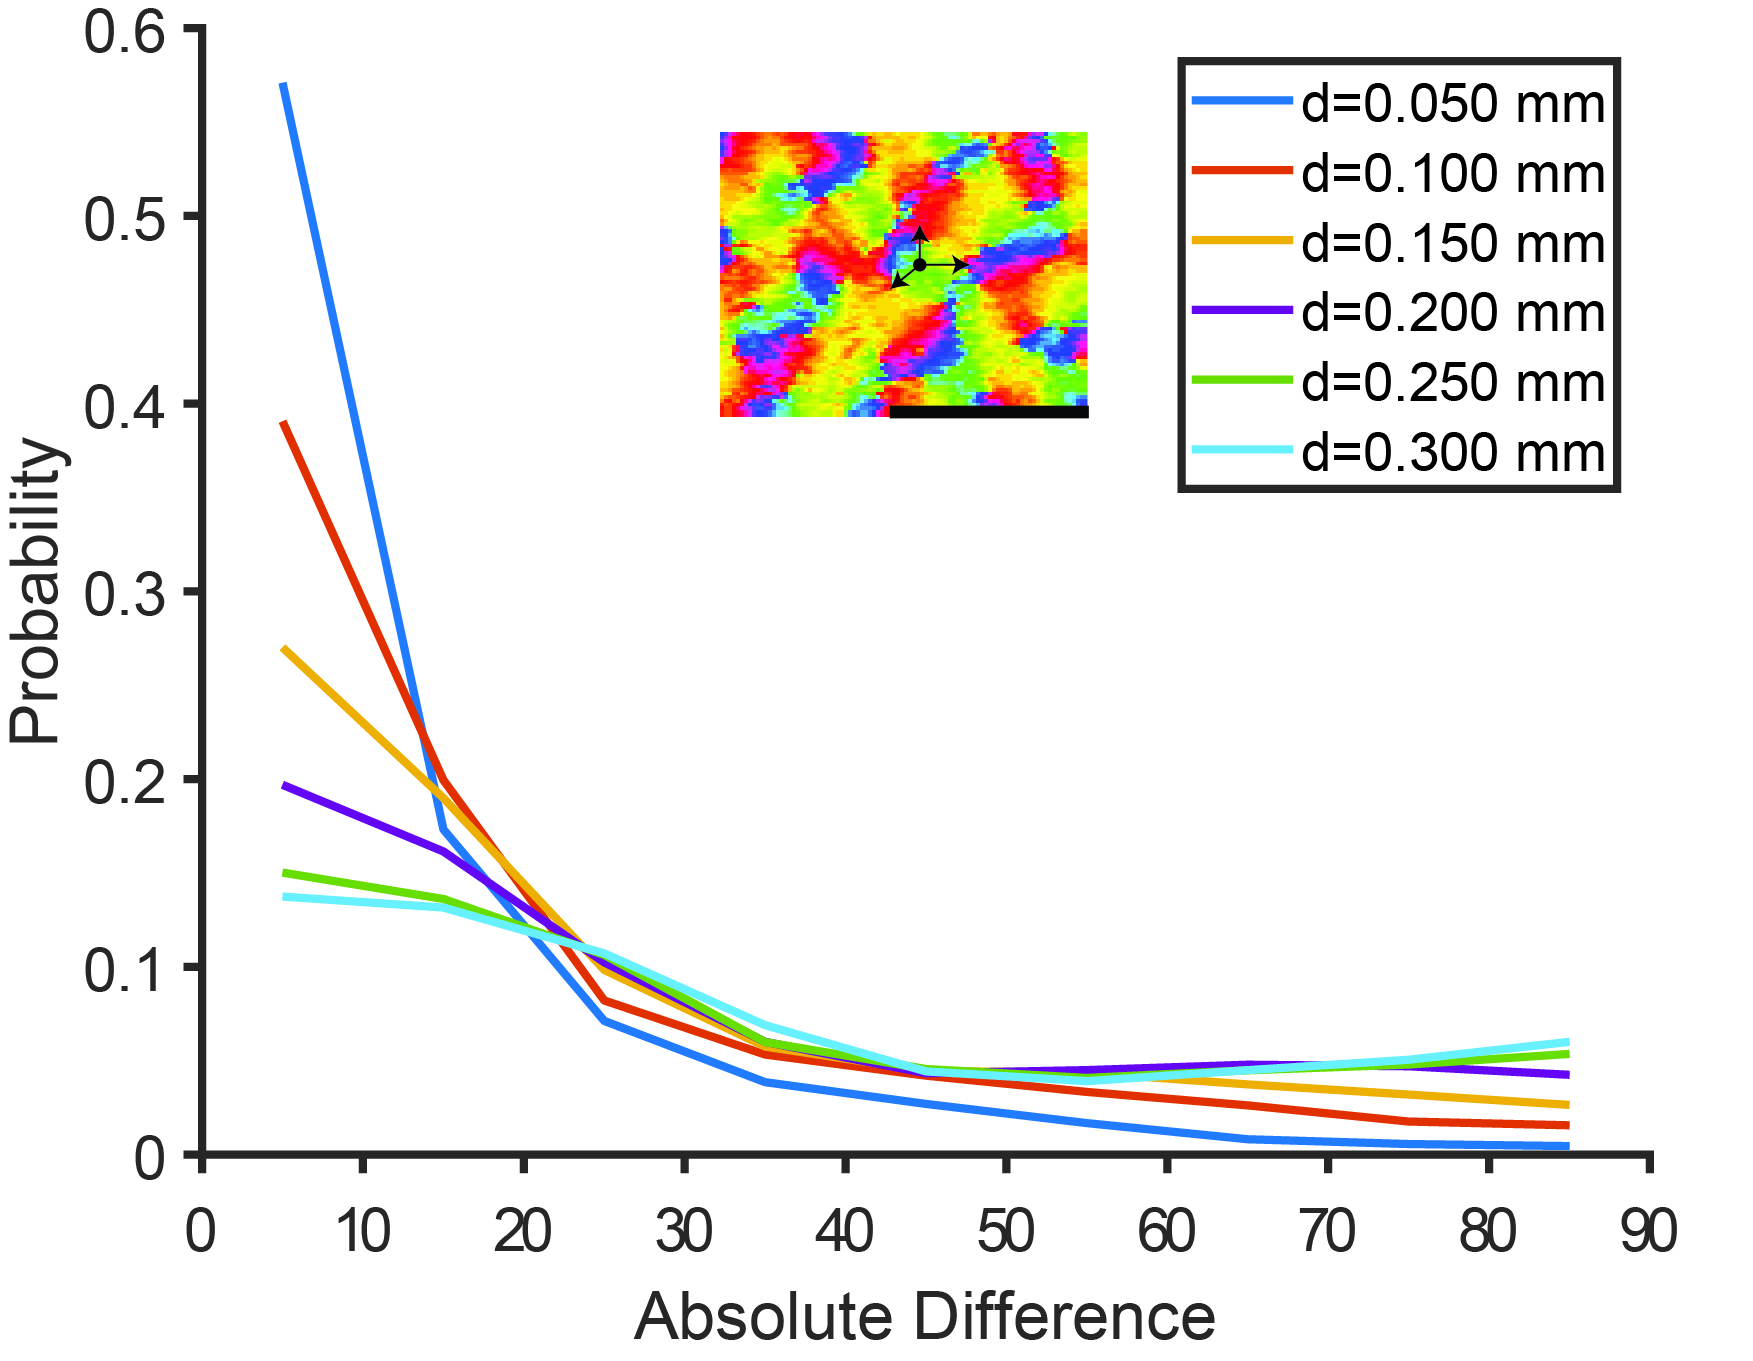
\includegraphics[width=0.6\linewidth]{ShrewV1/simulation.jpg}
	\caption{Results of a simulation experiment: The orientation tuning map (inset) was taken from Bosking et al., 1997. On this map, points were randomly placed and the orientation of 1000 pixels randomly selected at one of the distances in the legend was subtracted from the original data point. For each distance, the distribution of absolute differences for the 1000 pixels are shown by the lines in the graph. Black line is 1mm.}
	\label{fig:sim}
\end{figure}

\subsubsection{Spatial Frequency Tuning of neurons}

The distribution of the low cut-off, preferred and high cut-off spatial
frequencies of the neurons in layer 2/3 and layer 4 are shown in fig. 6.
Results from only these two layers are shown as we propose that the
orientation selectivity of layer 2/3 neurons arise predominantly from
layer 4 neurons. We found no significant differences between the spatial
frequency tuning between the two layers (n$_{23}$=27;
n$_{4}$=27; optimum spatial frequency: Wilcoxon rank sum,
z=-0.29, p=0.76; low cut-off: Wilcoxon rank sum, z=-0.75; p=0.45; high
cut-off: Wilcoxon rank sum, z=-1.69, p=0.09). although layer 2/3 neurons
tended to show high spatial frequency attenuation when compared to layer
4 neurons. When the bandwidth of spatial frequency tuning in octaves was
calculated, we found that the layer 2/3 neurons showed slightly sharper
tuning (median layer 2/3 b$_{oct}$= 2.2; n=16; median layer 4
b$_{oct}$=2.3; n=9). 11 of the 27 layer 2/3 neurons and 18 of
the 27 layer 4 neurons were low-pass tuned to spatial frequency.

		\begin{figure}[H]
	
	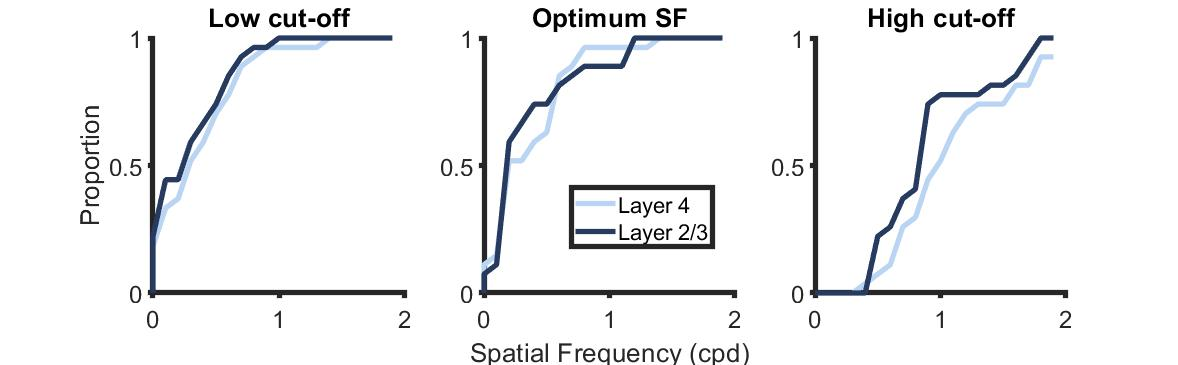
\includegraphics[width=\linewidth]{ShrewV1/sftuning_neurons_2.jpg}
	\caption{The cumulative distribution of the spatial frequency tuning of neurons in layers 2/3, 3c and 4 of the Shrew V1.}
	\label{fig:sftuning}
\end{figure}


In \textbf{[H2]}, we predicted that the layer 4 neurons will be more
tuned to orientation at higher spatial frequencies. We tested this
hypothesis by comparing the optimum spatial frequency tuning of layer 4
neurons with the spatial frequency where they demonstrated most
orientation tuning in 20 neurons. These results are presented in fig. 7.
Most neurons are located above the identity line, indicating that the
spatial frequency where they are maximally tuned for orietnation is
greater than the optimum spatial frequency of the neuron. The median
optimum spatial frequency of the layer 4 neurons was 0.35 cpd (95\% CI=
{[}0.2, 0.6{]}). The median of the spatial frequency where the
orientation selectivity index was the highest was 0.8 cpd (95\% CI=
{[}0.6, 1.2{]}). The spatial frequency at which the layer 4 neurons were
most tuned for orientation was significantly higher than the neurons'
optimum spatial frequency (Wilcoxon rank sum test, n=20, z= -2.93,
p\(<\)0.005).

\begin{figure}[H]
	
	\includegraphics[width=\linewidth]{ShrewV1/layer4OSI_highres.jpg}
	\caption{The relationship between the optimum spatial frequency of the layer 4 neurons and the spatial frequency at which the layer 4 showed the highest OSI. The dashed line is the identity line. The solid red line is the result of a linear fit of the form y=mx+c to the data (m= 0.73 [-0.15, 1.61] and c=0.58 [0.15, 1.01]). }
	\label{fig:OSI4}
\end{figure}


The results from 18 tracks where we compared the peak spatial frequency
of the layer 2/3 neurons and the spatial frequency where the layer 4
neurons were tuned for orientation are shown in fig.8. Fig 8a shows the
spatial frequency tuning curve of a layer 2/3 neuron and that of the
corresponding layer 4 neuron to the optimum and orthogonal orientation.
We hypothesised \textbf{{[}H3{]}} that the optimum spatial frequency of
the layer 2/3 neuron and the spatial frequency at which the layer 4
neurons was most tuned for orientation would be similar. We found that
this relation held true only in 3 of our 18 tracks. The median of the
optimum spatial frequencies of the layer 2/3 neurons was 0.2 cpd (95\%
CI= {[}0.1, 0.4{]}). In this sample of layer 4 neurons, the spatial
frequency where the neurons were most tuned to orientation was 0.8 cpd
(95\% CI= {[}0.3, 1.2{]}). In most of the tracks the maximum OSI of the
layer 4 neurons occured at higher spatial frequencies when compared to
the optimum spatial frequency of the layer 2/3 neuron (Wilcoxon signed
rank test, n=18, p\(<\)0.005) as demonstrated by the data points skewed
closer to the y-axis.

\begin{figure}[H]
	
	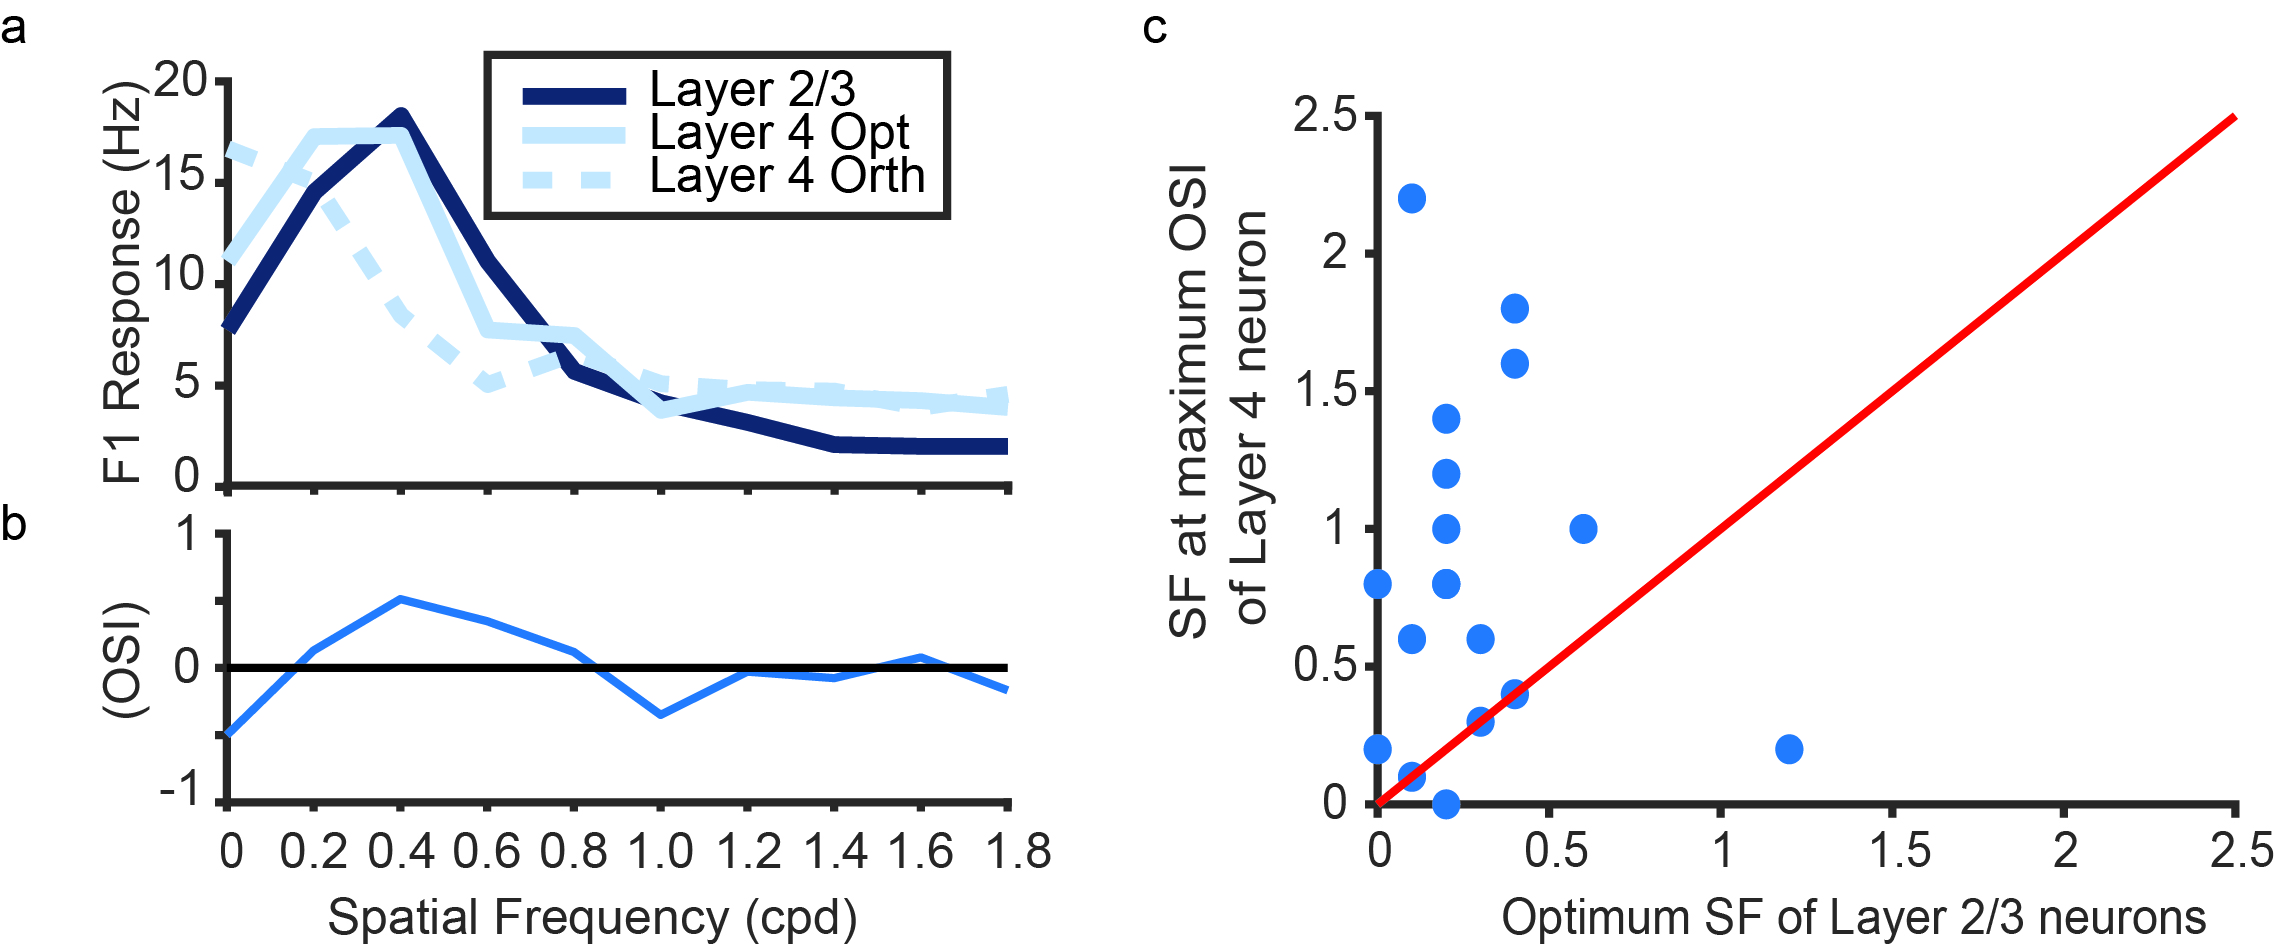
\includegraphics[width=\linewidth]{ShrewV1/sfsummary.jpg}
	\caption{The cumulative distribution of the spatial frequency tuning of neurons in layers 2/3, 3c and 4 of the Shrew V1.}
	\label{fig:sfsum}
\end{figure}



\section{Discussion}

In this chapter, we used extracellular recordings from layers 2/3 and
layer 4 of the tree shrew V1 to examine if orientation selectivity could
arise from sharpening the biased inputs from layer 4 neurons via the
ALD-RM model. As hypothesized, we found that the layer 4 neurons and the
layer 2/3 neurons were tuned to similar orientations \textbf{(H1)} and
that as the spatial frequency of the stimulus increased, the orientation
tuning of the layer 4 neurons got sharper \textbf{(H2).} In
\textbf{(H3)}, we hypothesised that the layer 2/3 neuron's peak spatial
frequency would be similar to the spatial frequency where the layer 4
neurons showed maximum orientation tuning. We found that this was only
true in three neuron pairs. These results are further discussed below.


\paragraph{Sharpening of orientation tuning in layer 2/3 and layer 4}

In this chapter, we determined the orientation selectivity of V1 neurons
from Layers 2/3, 3c and 4. We found that most neurons in layer 4 and
layer 3c were broadly tuned to orientation. While layer 2/3 neurons
showed sharper tuning to orientation overall, individual neurons showed
a bimodal distribution of orientation selectivity. These results are
consistent with previous results published in the tree shrews (Van
Hooser et al., 2013) and those published in the primary visual cortex of
macaques and cats where a wide range of orientation selectivities was
reported in V1 (Ringach et al., 2002).

In our study we used oriented bars to measure the degree of orientation
selectivity of neurons. Bars stimuli have a complex spatial frequency
spectrum and yield higher values of orientation selectivity when
compared to gratings of the optimum spatial frequencies (Reference). As
neurons showed better orientation selectivity to bars, it was easier for
us to determine the optimum orientation for further testing when bar
stimuli were used. However, it is likely that we have over-estimated the
extent of orientation selectivity, especially in layers 3c and 4 of
shrew V1. Van Hooser and colleagues also showed that there were two
groups of layer 4 neurons, those towards the edges of the layer 4 that
showed sharp orientation tuning and those in the middle that showed
broader orientation selectivity. In our sample (29 neurons), we only
found one layer 4 neuron that showed sharp orientation tuning, however,
this does not exclude the presence of more sharply tuned units at the
edges of layer 4.


\paragraph{Orientation columns in the tree shrew V1.}

In \textbf{H1}, we hypothesised that if the excitatory input from layer
4 neuron informed the orientation selectivity of the layer 2/3 neuron,
then both neurons will have the same optimum orientation. We found that
this was indeed the case. This also indicates that within an electrode
track, the columnar architecture observed in layer 2/3 might already be
present in layer 4. Surprisingly however, we found that layer 3c neurons
in V1 were tuned to an orientation 65\textsuperscript{o} away from the
optimum orientations of the layer 2/3 and the layer 4 neurons,
indicating that there is a laminar segregation in the optimum
orientation of neurons in the tree shrew V1. Neurons in this layer also
show broader orientation tuning unlike other layer 2 or 3 neurons. Here
we examine two possibilities for the difference in receptive field
properties of layer 3c neurons.

\textbf{Layer 3c is an input layer and is an extension of layer 4.}

The bottom of layer 3c neurons get inputs from layer 6 neurons in the
LGN in tree shrews. As a result, it has been suggested that this layer
might be an extension of layer 4, the LGN input layer in tree shrews
(Conley et al., 1984). Our results where the orientation biases of layer
3c neurons are similar to that of layer 4 neurons also supports this
hypothesis (also see Van Hooser et al., 2013). Further, it has also been
shown that while there are extensive horizontal connections within
layers 2-3b, layer 3c lacks horizontal connections, similar to layer 4.

\textbf{Layer 3c forms part of the koniocellular pathway in tree shrews.}

In macaques, layer 3B, which is located just above layer 4, contains
neurons that are broadly tuned to orientation. This layer receives
direct koniocellular inputs (from W-like cells) and shows blobs when
stained with cytochrome oxidase. As layer 3c cells receive inputs from
W-like cells, it has been suggested that layer 3c parallels layer 3b in
the tree shrew cortex. It is however important to note that it was layer
3b neurons and not layer 3c neurons in the tree shrew cortex that showed
patchy cytochrome oxidase staining. As a result, the pathway from W-like
cells in the retina via layer 3 of the LGN to layer 3B of V1 could be
the equivalent of the koniocellular pathway in macaques.

\textbf{Layer 3c provides cross orientation inhibition to layer 2/3 neurons.}

Another possibility could be that the neurons in layer 3c could be
providing inhibitory inputs to the layer 2/3 neurons. As we have shown
in this study, the layer 3c neurons show broader orientation selectivity
when compared to the rest of the layer 2/3 neurons and are tuned to an
orientation 65\textsuperscript{o} away from the orientation of the
corresponding layer 2/3 and layer 4 neurons. Layer 3c neurons are also
meant to receive inputs from the layer 4 (Fitzpatrick, 1996). Layer 3c
neurons could pool responses from the layer 4 neurons and provide the
basis for cross orientation inhibition in the layer 2/3 neurons rather
than both excitatory and inhibitory inputs arising from layer 4. If the
excitatory and inhibitory inputs from layer 4 and layer 3c neurons serve
to establish the initial orientation selectivity, then horizontal
connections in layer 2/3 could amplify the orientation response of the
neurons through recurrent excitation. This would also explain the
results of experiments where the stimulation of horizontal connections
had an additive effect rather than the modulatory effect previously
attributed to them (Huang et al., 2014).


\paragraph{Distribution of Spatial Frequency}

We also observed that spatial frequency tuning sharpened from layer 4 to
layer 2/3, however this sharpening was not statistically significant
(2.2 octaves to 2.3 octaves from layer 4 to layer 2/3). However,
bandwidth calculation could only be made in neurons that showed band
pass spatial frequency tuning. There was a significant change in the
number of layer 4 neurons that were low pass tuned to spatial frequency
(67\%) when compared to the layer 2/3 neurons (41\%). Of the bandpass
tuned neurons, layer 2/3 neurons also showed higher spatial frequency
attenuation. These results indicate that there was sharpening of
orientation selectivity from layer 4 to layer 2/3 in the tree shrew V1.

It is also important to note that when the low pass, optimum and high
pass spatial frequencies of neurons were compared, there was no
statistically significant differences between the three layers,
suggesting that the distribution of spatial frequency tuning stayed
similar throughout the primary visual cortex. Taken together with the
sharpening of spatial frequency tuning from layer 4 to layer 2/3
neurons, these results indicate that in most layer 2/3 neurons, there is
a direct sharpening of the inputs and the extensive low spatial
frequency attenuation reported in cats (Ref.) happens to a lesser extent
in tree shrews.


\paragraph{Spatial Frequency Dependence of Orientation Tuning}

We examined if the orientation selectivity of layer 4 neurons varied in
relation to the spatial frequency tuning of the neurons. We found that
in most cases, layer 4 neurons showed sharper orientation selectivity at
higher spatial frequencies as predicted in \textbf{(H2)}. In the tree
shrews then, orientation tuning of the layer 2/3 could be explained if
these neurons responded best at spatial frequencies where the layer 4
neurons were showed sharper orientation selectivity as suggested in
\textbf{(H3)}. However, when we tested \textbf{(H3)}, we found that it
was true only for a small proportion of neurons. In only 5 pairs of
neurons (out of 18) did the layer 2/3 neuron respond best at or above
the spatial frequency where the layer 4 neuron was best tuned to
orientation. In the other pairs, the layer 4 neurons were optimally
tuned for orientation at spatial frequencies higher than the optimum
spatial frequency of layer 2/3 neurons. What does it mean\ldots{}

In \textbf{(H3)} we hypothesised that the peak spatial frequency of the
layer 2/3 neurons would be similar to the spatial frequency where the
orientation tuning of the layer 4 neuron was greatest. We only found
this result in a small proportion of the neurons in our study. As a
result, while we cannot definitely conclude that neurons in layer 2/3
use non-specific inhibition to sharpen the orientation biases inherited
from the layer 4 neurons, we do have some evidence that suggests that
this could be the mechanism through which orientation arises in some
neurons in the tree shrew V1.

	

	\chapter [Orientation tuning in Superior Colliculus]{Orientation tuning in the Tree Shrew Superior Colliculus}

	\pagebreak
	\section{Summary}
	
	Though earlier theories of orientation selectivity suggested that orientation biases observed in V1 inputs are the result of excitatory convergence, studies have shown that these biases may be inherited from neurons in sub-cortical structures, namely the lateral geniculate nucleus (dLGN) and ultimately the retina. However, there is some controversy as to whether the biases reported in these sub-cortical structures arise from cortical feedback instead of biased inputs. If orientation selectivity arises from the retina, it should be evident in other targets of retinal projections. The superior colliculus (SC) is one such area. Here, orientation selectivity of SC neurons in tree shrews was measured using thin bars and gratings of different spatial frequencies. SC neurons showed orientation tuning and spatial frequency tuning comparable to that observed in the LGN of tree shrews. At higher spatial frequencies, the orientation selectivity was more evident, similar to that reported in the retina and LGN of cats and macaques. Similar results have also been reported in layer 4 of the tree shrews earlier in this thesis (see Chapter 5). These results indicate that the potential source of orientation biases in the LGN and the SC could be the retina. Direction selectivity and linearity of the SC neurons were also studied.
	
	\pagebreak
	
	
	\section{Introduction}
	
The tree shrew superior colliculus (SC) is a large well laminated structure (Tigges \& Shanta, 1969; Zhou et al., 2016). It is sub-divided into areas important for visual form processing and visuomotor processing (Casagrande et al., 1972; Casagrande \& Diamond, 1974) and has been implicated in an alternative pathway to the visual cortices (Killackey et al., 1971; Killackey \& Diamond., 1971). While the functional role and the projections of the SC have been extensively studied, few studies have characterised the receptive field properties of individual neurons. In this chapter, the receptive field properties, specifically orientation and spatial frequency tuning of the tree shrew SC neurons were studied and compared with the properties of the geniculo-striate system of the tree shrews.
 
Due to its extensive reciprocal projections to sensory as well as motor areas of the brain, the SC was implicated in oculomotor behaviour (Sherrington, 1947). However, studies where different layers of the SC were lesioned showed that the SC consisted of two separate functional systems --- the superficial layers essential for visual form discrimination and the inferior layers implicated in oculomotor function and orienting behaviour (Casagrande et al., 1972; Casagrande \& Diamond, 1974). The superficial layers of the tree shrew SC are further divided into stratum zonale (SZ), stratum griseum superficiale (SGS) and stratum opticum (SO) with the SGS further subdivided into upper and lower SGS (uSGS and lSGS respectively). As these are the layers of the SC that predominantly receive visual input (from the retina and primary visual cortex (V1); see May, 2006 for review), only the response properties of neurons in these superficial layers were studied.

In the present study, we aimed to examine orientation biases in the tree shrew SC. More than 50 years after its first report, the mechanism underlying orientation selectivity is still debated (Ferster \& Miller, 2000; Priebe \& Ferster, 2008; Scholl et al., 2013; Vidyasagar \& Eysel, 2015; Kremkow et al., 2016). The model of excitatory convergence proposed by Hubel \& Wiesel (1962, 1968) for orientation selectivity in cats and macaques assumed that orientation selectivity was first generated in the primary visual cortex along the visual pathway. A similar mechanism, where orientation selectivity is generated for the first time in layer 2/3 of the primary visual cortex has been proposed in the tree shrews (Chisum et al., 2003; Mooser et al., 2004) These theories have largely ignored the orientation biases that have been demonstrated in sub-cortical areas. Subcortical orientation biases have been reported in the retina and the dLGN of most species (cats- Levick \& Thibos, 1980; Vidyasagar \& Urbas, 1982; Levick \& Thibos, 1982; Shou \& Leventhal, 1989; macaques- Smith et al., 1991; Xu et al., 2002, Passaglia et al., 2002; tree shrews- Van Hooser et al., 2013; rodent- Tan et al., 2011; Sun et al., 2016). However, oriented neurons in the superior colliculus have only been reported in rodents (Wang et al., 2010; Inayat et al., 2015; Ahmadlou et al., 2015; Shi et al., 2017). In cats and macaques, direction selectivity has been reported in the Superior Colliculus (McIlwain \& Buser, 1967; Sterling \& Wickelgren, 1969; Rosenquist \& Palmer, 1971; Cynader \& Berman, 1972; Goldberg \& Wurtz, 1972), but units can be selective to direction without being selective to orientation (see figure 6a and 6b in results). In one detailed study that examined receptive field properties in the tree shrew SC, a small proportion (~20\%) of SC neurons were orientation tuned (responded three times better at optimum orientation compared to the non-optimum orientation) in the superficial layers of the SC (Albano et al., 1978). A recent study in the tree shrew geniculostriate system however, showed that nearly 50\% of tree shrew LGN neurons showed orientation biases (Van Hooser et al., 2013), albeit to a smaller extent than that reported by Albano et al. (1978). In this chapter, the orientation biases of the shrew SC were characterized using bars and gratings and compared to that of the shrew LGN.

Since neurons in the superficial SC receive inputs from both retina and the primary visual cortex, we further characterized the receptive field properties of the SC neurons so as to infer their source. Certain properties of the SC neurons such as binocularity, direction selectivity and colour selectivity have been attributed to cortical feedback in carnivores and primates (Sterling \& Wickelgren, 1969; Cynader \& Berman, 1971; Tailby et al, 2012). In the rodents however, it has been shown that direction and orientation selectivity were inherited directly from the retinal projections on to the SC neurons (Shi et al., 2017). Therefore, one key aim of this experiment was to determine whether the receptive field properties of SC neurons were more similar to those of the retinal neurons or cortical neurons. Neurons of the primary visual cortex show sharp orientation selectivity and a bandpass spatial frequency tuning (Movshon et al., 1978a; Movshon et al., 1978b; Movshon et al., 1978c; DeValois et al., 1982). Retinal and LGN neurons are broadly tuned to orientation and have a low pass spatial frequency tuning. At higher spatial frequencies, neurons from both regions show sharper orientation tuning (Enroth-Cugell \& Robson, 1966; Levick \& Thibos, 1980; Levick \& Thibos, 1982; Vidyasagar \& Urbas, 1982; Vidyasagar \& Heide, 1984; Shou \& Leventhal, 1989). Here, we examined the orientation and spatial frequency responses of the neurons of the superior colliculus.

As we propose that asymmetries in the feedforward signal are elaborated by the target neurons to elaborate feature selectivity (Vidyasagar \& Eysel, 2015), we predicted that the SC and the LGN neurons in the tree shrews, will respond similarly.  Accordingly, the following hypotheses were tested.


\noindent{\textbf{(H1)}: Superficial SC neurons will show oriented responses when shown thin bars (which contain high spatial frequency information).}

\noindent{\textbf{(H2)}: Superficial SC neurons will have low pass spatial frequency tuning, similar to their LGN counterparts, when tested using sinusoidal gratings.}

\noindent{\textbf{(H3)}: When gratings of different spatial frequencies are used, a similar proportion of superficial SC and LGN neurons will be orientation tuned. The SC neurons will also show an orientation selective response at higher spatial frequencies.}

	
	\section{Methods}
	\subsubsection{Surgery and anaesthesia}
Surgical procedures have been outlined in detail in the Methods chapter.
Briefly, the animals were anaesthetized using a mixture of Ketamine and
Xylazine, a venous catheter was inserted in to the femoral vein and a
tracheostomy performed to assist in breathing during the experiment. The
animal was administered muscle paralysant (Vecuronium Bromide)
intravenously and was anaesthetised using Isoflurane (0.5-1\%) for the
duration of the experiment. Hard contact lenses were fitted to the eye
to prevent corneal drying. A craniotomy and durotomy were performed over
the location of the SC (Horsley-Clarke Co-ordinates A2.5 to P2.5).
Frontal EEG and ECG were monitored during the experiment. At the end of
the experiment, the animal was euthanized using an overdose of
pentobarbital sodium and perfused (using 0.1M Phosphate Buffer (PB)
solution followed by 4\% Paraformaldehyde in 0.1M PB), the brain was
removed and stored in sucrose (20-25\%) for histology.

	\subsubsection{Electrophysiology}
High impedence, lacquer coated tungsten microelectrodes (FHC Metal
Microelectrodes Inc., ME, USA; impedance= 12-18 M$\Omega$) were lowered into
the brain and the signal was amplified and filtered (x 10,000 gain,
bandpass filtered between 300-3000 Hz, A-M systems) and fed into an
audio speaker as well as an analog to digital converter (Cambridge
Electronic Design Limited, Cambridge, UK; digitised at 22.5 kHz). The SC
was identified by listening to the neuronal activity in the speaker. The
electrode was first quickly descended to a depth of 3 mm and then slowly
descended until visual neurons were identified. Lesions (6 μA for 6s)
were made at the end of each track. When thehe electrode was withdrawn
and lesions were made at regular intervals to trace the path of the
electrode through the brain. The data was recorded using the spike 2
software (CED, Cambridge, UK). The spikes were templated and the spike
timing exported as a text file. Further analysis was performed using
custom MATLAB code (The Mathworks Inc, USA).
	\subsubsection{Stimuli}
Stimuli were presented using a BARCO monitor (Frame Refresh Rate= 80 Hz;
Reference Calibrator Plus; Barco Video and Communications, Belgium)
centred on the neuron's receptive field and generated using Visage (VSG,
Cambridge Research Systems, Cambridge, UK) and custom Stimulus
Description Language (SDL) scripts. The monitor had a mean luminance of
32.6 cdm\textsuperscript{-2}. While recording, the monitor was placed at
a distance of 114 cm from the eye. For each of the different stimuli
described below, ten complete stimulus presentations were completed.

For each SC neuron, the preferred stimulus orientation was initially
measured using a thin moving bar. The bar was presented in 9 different
orientations sweeping bi-directionally (a total of 18 orientations). The
background was a uniform gray screen. Depending on the polarity of the
neurons, either a bright bar or a dark bar was used (contrast= 100 \%).
The bar was usually 8\textsuperscript{o} long (ranging between 4 and 8
degrees) and 0.5\textsuperscript{o} wide (ranging between 0.1 and 1
degree). The velocity of the bar was between 5 and 20
\textsuperscript{o}/second. The width of the bars were usually reduced
until an oriented response was observed. Where the thinnest bar we
presented did not elicit an oriented response during the experiment, the
neuron was classified as unoriented.

Peri-stimulus-time-histograms (averaged over 10 trials, 20 ms bin-width;
PSTHs) were generated using the spike 2 software for online analysis.
Based on the PSTHs generated following the presentation of the bar, the
optimum orientation of the neuron was determined and used for further
testing.

The spatial frequency responses to gratings were then measured. The
animals were presented with drifting sine-wave gratings (Temporal
Frequency= 4Hz; Contrast=100\%) of varying spatial frequencies (SF; SF
between 0 cycles per degree (cpd) to 2 cpd) at atleast two different
orientations (optimum, optimum + 90\textsuperscript{o}). Where we could
perform stable recordings, SF responses at two more orientations
(optimum+45 \textsuperscript{o}, optimum-45 \textsuperscript{o}).
	
	
	\subsubsection{Data Analysis}
	
	Regardless of the stimulus presented, the following analysis was performed on the extracellular trace before any specific analysis was undertaken. Spikes were templated and the spike time and stimulus markers were exported into text files. Using custom scripts in MATLAB, PSTHs (bin-width= 20ms) were constructed for each of the stimulus conditions.  Spike density functions were created using a moving Gaussian envelope with σ of 60 ms (3 bins). This SDF was used for further analysis.
	
	\paragraph{Analysis of Bar Stimuli Responses}
	
Regardless of the stimulus presented, the following analysis was
performed on the extracellular trace before any specific analysis was
undertaken. Spikes were templated and the spike time and stimulus
markers were exported into text files. Using custom scripts in MATLAB,
PSTHs (bin-width= 20ms) were constructed for each of the stimulus
conditions. Spike density functions (SDFs) were created using a moving
Gaussian envelope with σ of 60 ms (3 bins). This SDF was used for
further analysis.

{Analysis of Bar Stimuli}

For orientation tuning recorded using a bar, the peak response in the
SDF for each direction of movement was plotted on a polar diagram. The
circular variance (CV; Ringach et al., 2002) and the orientation bias
(bias, Vidyasagar \& Urbas, 1982) were also calculated as follows:

\begin{equation} \label{cv}
CV=1 - |\frac{\text{mean}\left( r*e^{(i*2\mathbf{\theta})} \right)}{\text{mean}\left( r \right)}|
\end{equation}

Where θ is the direction of movement of the bar (between 0 and 340
degrees) and r is the response at that direction. A CV value of 0 meant
that the neuron was sharply tuned to orientation and a circular variance
value of 1 meant that the neuron responded equally at all orientations.
In this study, neurons with a CV greater than 0.9 were classified as
unoriented neurons (Ringach et al., 2002).

\begin{equation} \label{bias}
Bias=\frac{R_{\text{opt}}}{R_{\text{orth}}}
\end{equation}


Where R$_{opt}$ is the response of the neuron to the optimum
direction of movement and R$_{orth}$ is the response of the
neuron to the orientation 90 degrees away from the optimum direction of
movement. Unoriented neurons have a value close to 1 and oriented
neurons can have bias values upto Infinity.

Direction selectivity of the neurons was also calculated using two
different methods to enable comparison with previous studies in the
superior colliculus. First, the direction selectivity index (DSI) was
calculated by taking the ratio of the response at the optimum direction
of movement and the response at the opposite direction of movement
(Goldberg \& Wurtz, 1972). Neurons whose DSI was less than 0.5 (i.e.
response in the opposite direction less than half of the response in the
optimum orientation) were classified as direction selective. In the
second method, the following formula was used to measure the directional
circular variance (DCV; VanHooser et al., 2013).

\begin{equation} \label{DCV}
DCV=
1 - |\frac{\text{mean}\left( r*e^{\left( i*\mathbf{\theta} \right)} \right)}{\text{mean}\left( r \right)}|
\end{equation}

Conventions are as described for the calculation of circular variance
(Equation \ref{cv}). Once again neurons that had a DCV less than 0.5 were not
direction selective.

{Analysis of Grating Stimuli}

For gratings, the Discrete Fourier Transform (DFT) of the spike density
function was calculated using the MATLAB Fast Fourier Transform
algorithm (FFT). The F1 and the F0 components of the response were
calculated (see General Methods for details) and the modulation index
(Van Hooser et al., 2013) was calculated as follows:

\begin{equation} \label{MI}
Modulation ratio=
2*\frac{F1}{(F1 + F0)}
\end{equation}

Where F1 is the value of the modulated component at the peak spatial
frequency and F0 is the value of the unmodulated component at the peak
spatial frequency. If the modulation ratio was less than 1, the cell was
considered to show non-linear summation over its receptive field and the
unmodulated component of the response was used for further analysis. If
the ratio was greater than 1, the cell was considered to show linear
summation and the F0 component of the response was used.

In order to characterize the spatial frequency tuning response of the
neurons, the peak spatial frequency of the neuron was taken as the
spatial frequency where the firing rate was maximum. In most cases, the
F0 and F1 components of the response peaked at the same spatial
frequency. However, in some cases, the peak spatial frequencies of the
F1 and F0 components were different. In these cases, if the F1 response
was significantly greater than the F0 response, the peak spatial
frequency of the F1 response was used. Otherwise, the peak spatial
frequency of the F0 response was used. The lower cut-off was the
frequency lower than the peak spatial frequency that gave a response
that was half the magnitude of the peak response. If the response did
not reach half the maximum response, the neuron was classified as a low
pass tuned neuron. The high cut-off was the spatial frequency higher
than the peak spatial frequency where response was half the magnitude of
the peak response. The spatial frequency tuning bandwidth was then the
difference between the high cut-off and the low cut-off spatial
frequencies.

In order to see if the neurons showed sharper orientation tuning at
higher spatial frequencies, first the spatial frequency tuning curve at
the optimum and orthogonal orientations were generated and the bandwidth
where the superior colliculus neurons responded for the optimum
orientation but not for the orthogonal orientation was calculated. In
order to do this, a `minimum response' was defined as the response where
the neurons fired similarly for the optimum and the orthogonal
orientations. The spatial frequencies where the response rate for the
optimum and orthogonal orientations first reached the minimum response
were termed the optimum cut-off and orthogonal cut-off and their
difference was calculated (see figure 1).
	
		\begin{figure}[H]
		
		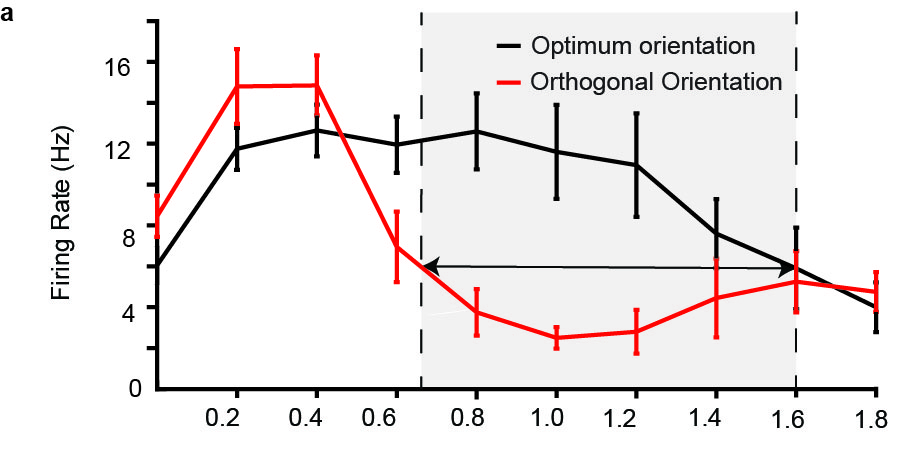
\includegraphics[width=\linewidth]{superiorcolliculus/SCOptOrth.jpg}
		\caption{Example SF tuning curves for optimum (blue) and
			orthogonal (red) orientations. The cut-off frequency at the optimal
			orientation is the SF at which the response at optimal orientation is no
			longer significantly different from the response at orthogonal
			orientation. The response at the cut-off frequency for optimum
			orientation is called the minimum response. For the orthogonal
			orientation, the cut-off frequency was the SF at which minimum response
			was first reached. Error bars are 95\% confidence intervals.}
		\label{fig:scoptorth}
		\end{figure}
	
Circular variance of the neurons at each spatial frequency was also
calculated using Equation 1 where spatial frequency tuning data for at
least four different orientations was recorded. The orientation
selectivity index (OSI) at each spatial frequency was also calculated as
1- reciprocal of orientation bias (Equation 2). The OSI instead of the
bias was calculated in this instance as 1) no comparison to previous
studies were made using this data; 2) The value of OSI would always be
within 0 and 1 whereas the maximum value of bias could be infinity; and
3) As this calculation only requires the spatial frequency data at the
optimum orientation and orthogonal orientations, a more complete data
set to examine the relationship between orientation tuning and the
spatial frequency tuning was present. The relationship between the OSI
and CV were also examined in the results.

	
	\subsubsection{Histology}
The brain that was stored in the sucrose at the end of the experiment,
was cut into 50 micron sections using a cryostat and then mounted on
gelatinised slides. The sections were then stained using Cresyl Violet
acetate solution. Lesions were identified and the electrode tracks
reconstructed using Adobe Illustrator to verify that all our neurons
were indeed recorded from the superior colliculus.
	
	\section{Results}
	
A total of 22 units were recorded from five tracks in three
anaesthetised Tree Shrews (2 female and 1 male). All neurons were from
the superficial layers of the SC. Of the 22 neurons, 20 were biased for
orientation. Spatial frequency tuning information was collected for 16
units, 12 of which showed low pass spatial frequency tuning. 13 of the
16 neurons also showed sharper orientation tuning at higher spatial
frequencies.
	
	
	\subsubsection{Anatomical location of units}
	
	The laminar position of all the units was determined by reconstructing
	the electrode tracks from the electrolytic lesions. The photomicrograph
	of a Nissl stained section from the SC is presented in figure 2a. The
	laminar position of the neurons determined from the electrode track
	reconstructions is shown in Figure 2b. All the recorded neurons were
	from the superficial layers, with the majority from the
	SGS.
		
	\begin{figure}[H]
		
		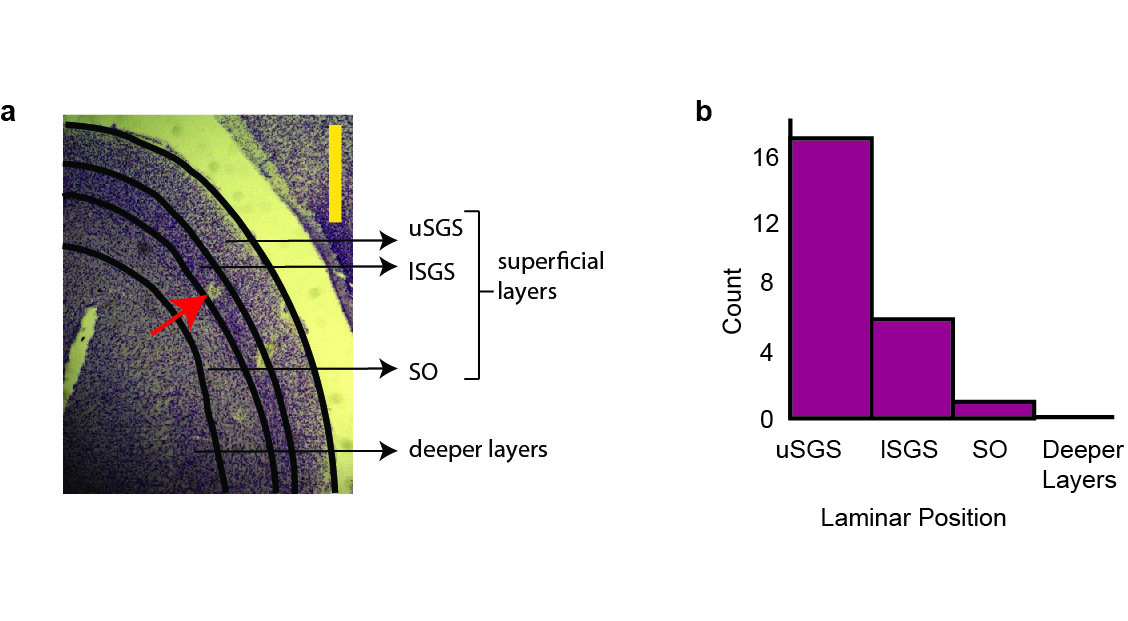
\includegraphics[width=\linewidth]{superiorcolliculus/anatpos.jpg}
		\caption{Laminar position of the neurons. (a) A photomicrograph of a tree shrew superior colliculus from the right hemisphere showing the different subdivisions of the superficial layers. The red arrow points to a lesion. Two other lesions from a different track are visible to the right of the lesion. The yellow scale bar is 1mm. (b) Number of cells sampled from each layer. Majority of the cells were from uSGS. Abbreviations: uSGS- upper Stratum Griseum Superficiale; lSGS- lower Stratum Griseum Superficiale; SO- Stratum Opticum.}
		\label{fig:anatpos}
	\end{figure}
	
	
	
	\subsubsection{Orientation Selectivity using bars}
	

The distribution of two measures of orientation selectivity are shown in
Figure \ref{fig:orihist}. Figure \ref{fig:orihist}a shows the distribution of circular variances. The
median circular variance for the sample was 0.80 (95\% confidence
interval(CI)= {[}0.70, 0.82{]}). The orientation tuning curves of a
representative neuron as well as those of the most selective, least
selective neuron with CV less than 0.9 and the least selective neuron in
the entire sample are presented in figure \ref{fig:range}a and b.

	\begin{figure}[]
	
	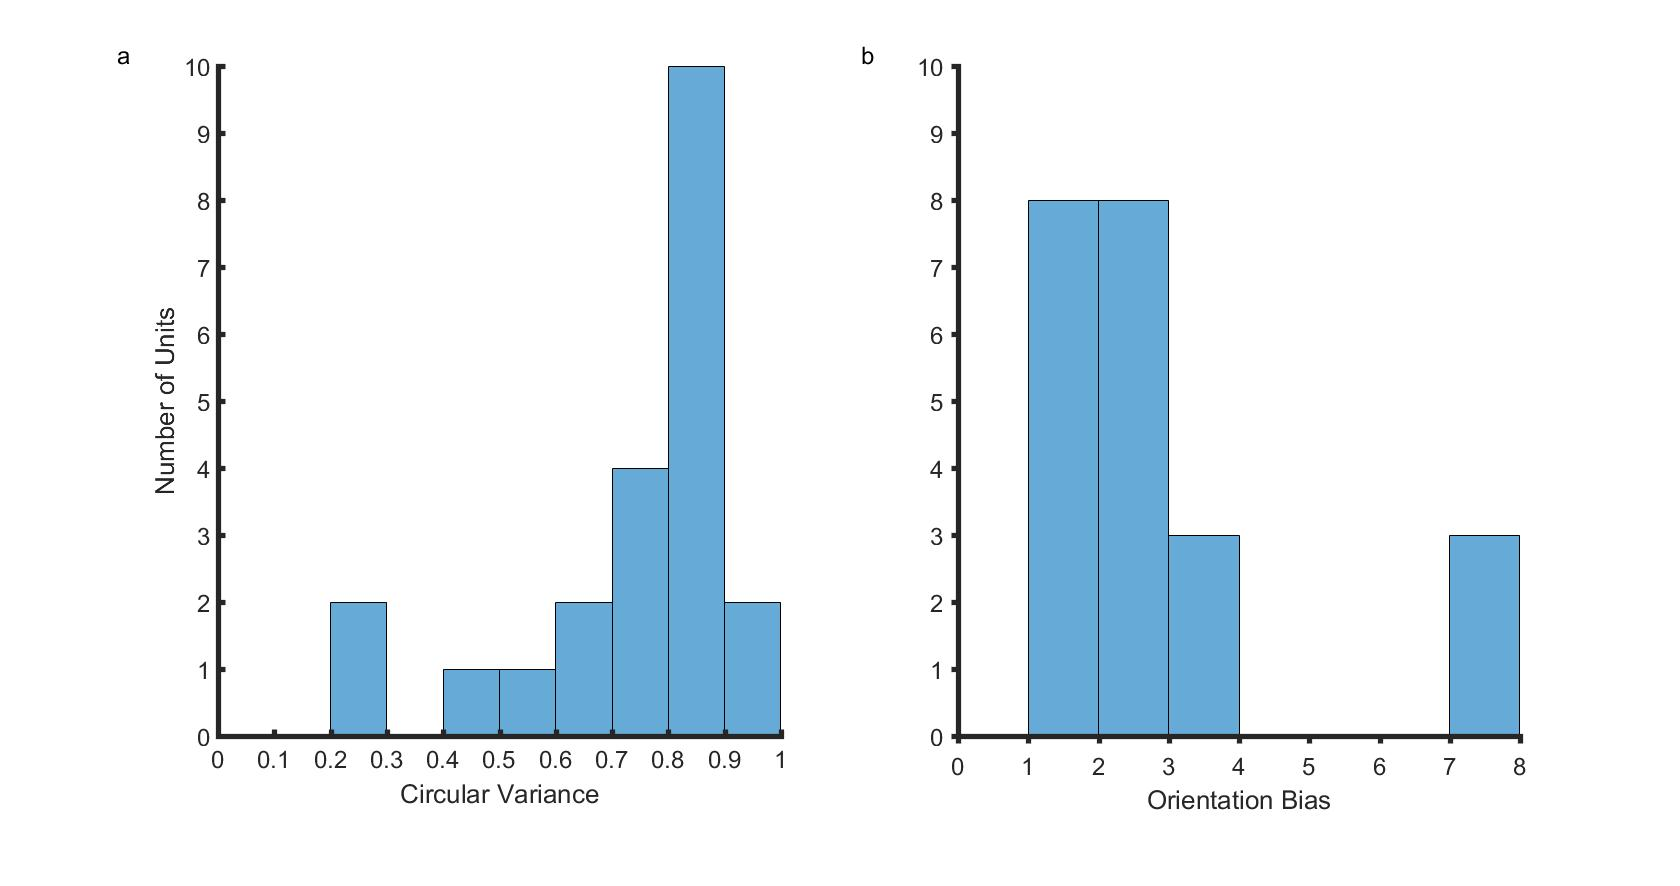
\includegraphics[width=\linewidth]{superiorcolliculus/orituning_fig.jpg}
	\caption{Orientation selectivity of neurons (a) This
		figure shows the distribution of circular variances of all neurons. (b)
		This figure shows the distribution of orientation biases.}
	\label{fig:orihist}
\end{figure}


\begin{figure}[]
	\includegraphics[width=\linewidth]{superiorcolliculus/cv.jpg}
	\caption{Orientation selectivity when measured with bars. (a) The
		orientation tuning of a representative neuron. The direction of movement
		of the bars are shown at the poles of the plot. The number next to the
		plot is the circular variance. The maximum firing rate of the neuron was
		117 spks/s. (b) Orientation selectivity of the sharpest, least tuned
		neuron included for further analysis and the least tuned neuron in the
		entire sample. The direction of movement of the bar are similar to (a).
		The circular variance of each neuron is displayed below. Maximum firing
		rate for the three neurons are 18 spks/s, 57 spks/s and 89 spks/s
		respectively. The response shown is the average of 10 trials and the
		error bars are ± 2*SEM. (c) the distribution of circular variances of
		all neurons in relation to the laminar position of the neuron.}
	\label{fig:range}			
\end{figure}

Any neuron with CV greater than 0.9 was classified as not selective to
orientation. Two neurons had a CV greater than 0.9 and hence were not
further recorded from.

An additional measure of orientation selectivity, the orientation bias
(Bias; figure \ref{fig:orihist}b) was also calculated. The median bias was 2.31 (95\%
CI={[}1.85, 3.20{]}). A bias of one would indicate that the response of
the neuron at the optimum and orthogonal orientations were the same.
Therefore, lower values of bias indicated that the neurons were more
broadly tuned. The two neurons that had circular variances greater than
0.9 had bias values closer to 1 (1.16 and 1.26). The orientation bias
was calculated to enable comparison with previous studies and further
analysis was not conducted using these values.

We also examined if there were any laminar differences in the
orientation biases, the circular variance of the neurons were also
plotted against the laminar position in figure \ref{fig:range}c. The neurons that
showed the sharpest orientation tuning were all located in the uSGS.	
	

	
	
	\subsubsection{Direction selectivity of neurons}
The distribution of the DSI and the DCV of 22 neurons are shown in
Figure \ref{fig:ds}a and b. All 22 neurons were included in the analysis as neurons
that are not tuned to orientation can be tuned to direction. Figure \ref{fig:dseg}a
shows a neuron that is selective to both orientation and direction. \ref{fig:dseg}b
shows a neuron selective to direction but not to orientation. The median
DSI was 0.69 (95\% CI= {[}0.5, 0.83{]}), suggesting that the majority of
the neurons were not direction selective. Of the 22 neurons that were
recorded from, only 5 (\textasciitilde{}20\%) satisfied our criteria for
direction selective neurons. The distribution of the DCV is shown in
figure \ref{fig:ds}b. The median DCV was 0.90 (95\% CI= {[}0.85, 0.93{]}). The DCV
was a more conservative measure of direction selectivity and none of the
neurons we measured from were selective to direction using this measure.
	
	\begin{figure}[H]
		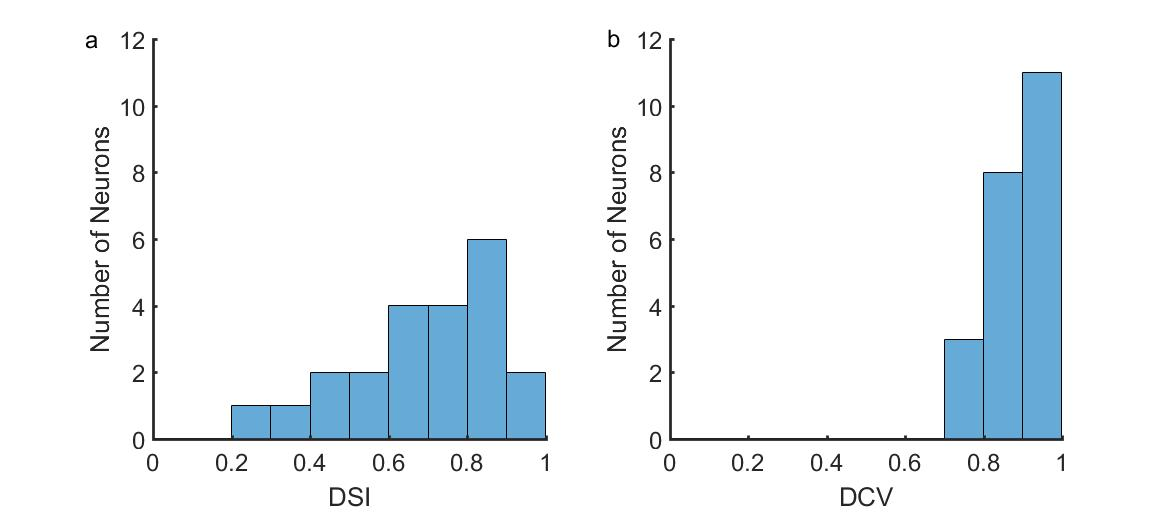
\includegraphics[width=\linewidth]{superiorcolliculus/directionselectivity_fig.jpg}
		\caption{Distribution of direction selectivity index of 22
				superior colliculus neurons using two different measures: the DSI (a)
				and the DCV(b).}
		\label{fig:ds}			
	\end{figure}
	
	\begin{figure}[H]
		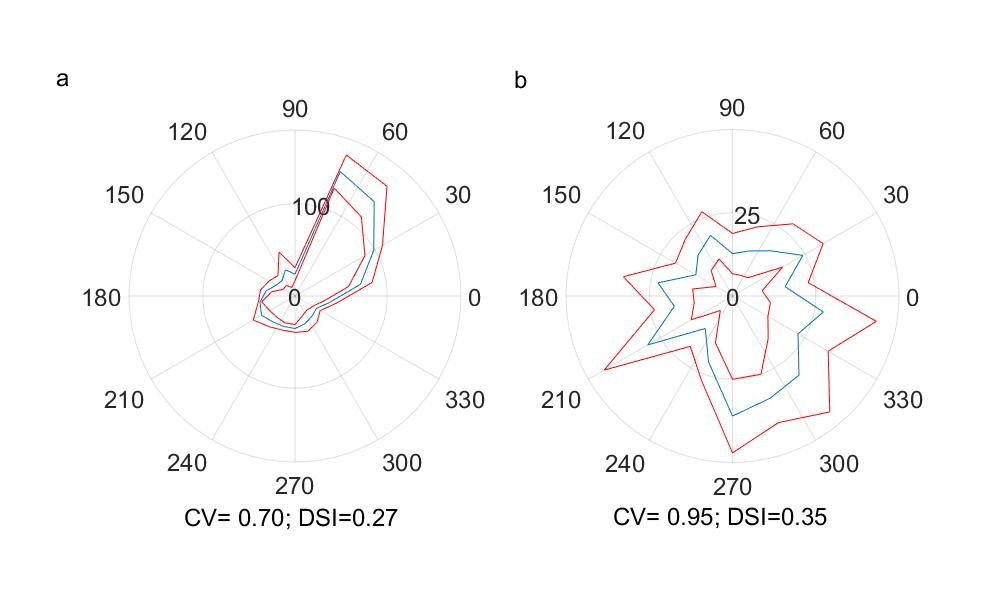
\includegraphics[width=\linewidth]{superiorcolliculus/Directionselectivity.jpg}
		\caption{Example of a cell that is selective to both direction
			and orientation (a) and a cell that is selective to direction but not
			orientation (b)}
		\label{fig:dseg}			
	\end{figure}
	
	\subsubsection{Spatial Frequency Tuning}
	
A summary of the results of spatial frequency tuning we obtained from 16
neurons is presented in figure 7a. The results from the LGN from Van
Hooser et al., 2013, Figure 7b, 30 neurons) were plotted on similar axes
in figure 7b to aid direct comparison. The median peak spatial frequency
of the SC neurons was 0.2 cpd (95\% CI= [0, 0.2]) and the median
half width at half height was 0.35 cpd (95\% CI= [0.15, 0.55]). SC
neurons tended to have higher spatial frequency cut-offs when compared
to the LGN neurons (figure 7b). A similar proportion of SC (80\%) and
LGN (76\%) neurons were low-pass tuned to spatial frequency .
	
	\begin{figure}[]
		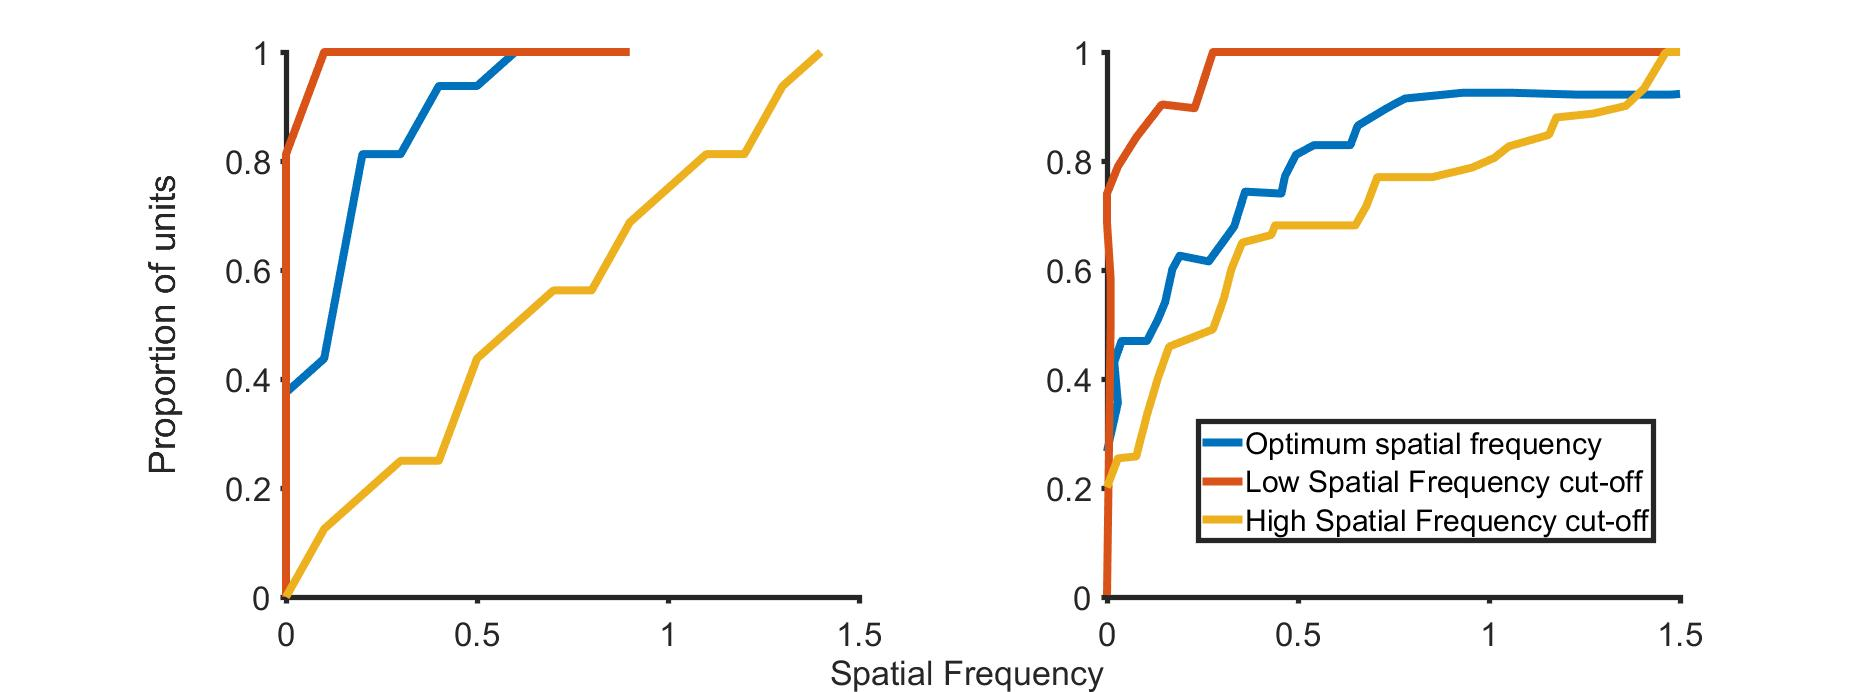
\includegraphics[width=\linewidth]{superiorcolliculus/cumsum_sf_SC_LGN.jpg}
		\caption{Cumulative distribution of the low-cutoff,
			optimum and high cut off spatial frequencies in the tree shrew Superior
			Colliculus for 16 neurons (a) and the Lateral Geniculate Nucleus for 30
			neurons (b; LGN). The LGN results were published in the paper by Van
			Hooser et al., 2013 (figure 7b) and plotted on the same scale as the SC
			data in the left hand side panel.}
		\label{fig:sfcumdist}			
	\end{figure}
	
	
	\subsubsection{Orientation tuning using gratings}
	
The circular variance of the orientation response of eleven neurons was
calculated at the peak spatial frequency and compared with those of
previously published data in the geniculostriate system of the tree
shrews. The distribution of these circular variances are shown in figure
8. The median CV of SC neurons when measured using gratings was 0.84
(95\% CI= {[}0.77 0.91{]}). The distribution of the CVs of the superior
colliculus and the LGN were similar. While in the LGN nearly 50\% were
not tuned to orientation at the peak spatial frequency, only 30\% of the
SC neurons did not show orientation tuning (1-CV\textless{}0.1). None of
the neurons demonstrated sharp orientation tuning (1-CV\textgreater{}
0.5) as observed in layer 2/3 of the cortex.
		
	\begin{figure}[]
		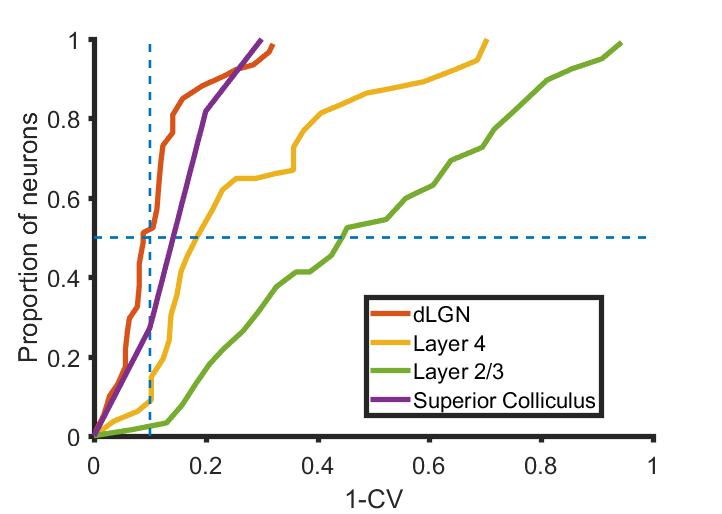
\includegraphics[width=\linewidth]{superiorcolliculus/orientation_bias_SG_geniculostriate_2.jpg}
		\caption{ Comparison of the distribution of the orientation
			selectivity of the LGN, Layer 4 and Layer 2/3 neurons to the
			distribution of orientation selectivity of the superior colliculus
			neurons. Horizontal dotted line indicates the 50\% of neurons and the
			vertical dotted line is the orientation tuning cut off.}
		\label{fig:CVvanhooser}			
	\end{figure}
	
As there was only enough data in 11 neurons to enable circular variance
calculations, the orientation selectivity index (OSI) was calculated for
the 16 neurons, where gratings of both optimum and orthogonal
orientation were calculated. The relationship of the OSI and the CV for
the 11 neurons where both these data were available is shown in figure \ref{fig:CVvOSI}. 
	
		\begin{figure}[]
		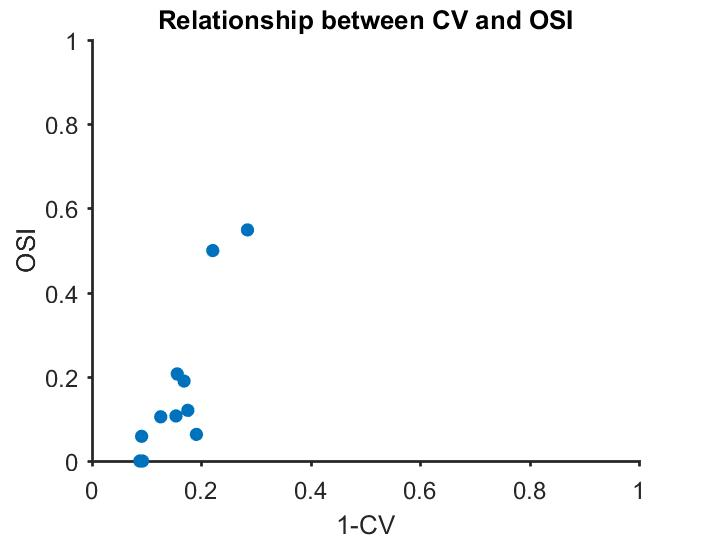
\includegraphics[width=\linewidth]{superiorcolliculus/CVvsOSI.jpg}
		\caption{Relationship between the circular variance and
			orientation selectivity index}
		\label{fig:CVvOSI}			
	\end{figure}
	
	Levick and Thibos (1982) calculated the circular variance of the neurons
	in their study at different spatial frequencies and found that neurons
	showed sharper tuning at spatial frequencies higher than the optimum
	spatial frequency. Since the circular variance and orientation
	selectivity index show a strong correlation (r= 0.87, p\textless{}0.005,
	n=11), in this chapter, OSI was used to conduct a similar analysis.
	
	\subsubsection{Relationship between spatial frequency and orientation tuning.}
	When the spatial frequency tuning response of the neuron at different
	orientations was measured, 13 of 16 neurons were tuned to orientation at
	higher spatial frequencies. The F0 components of a neuron's response to
	gratings of increasing spatial frequencies at the optimum and the
	orthogonal orientations are shown in figure \ref{fig:scoptorth}. The gray shaded area
	represents the spatial frequencies where the neuron still responds to
	gratings of the optimum orientation but no longer responds when gratings
	of the orthogonal orientation are presented (i.e., the neuron is
	orientation tuned). The difference in response between the optimum and
	non-optimum orientation cut off frequencies was calculated. These
	results for the group are presented in figure \ref{fig:sf_bw}. A one tailed Wilcoxon
	Signed Rank test showed that the spatial frequency cutoff at the optimum
	orientation was significantly higher than the spatial frequency cutoff
	at the orthogonal orientation (median difference= 0.4 cpd; z=3.15;
	p=0.0008). The magenta circles in figure 10 show the peak spatial
	frequency of the respective neuron and the green circles, the spatial
	frequency where the neuron was most tuned to orientation (where the OSI
	was maximum). The spatial frequency where the orientation tuning of the
	neuron was greatest was significantly higher than the peak spatial
	frequency of the neuron (One-tail Wilcoxon Signed Rank test; z=3.3096;
	p=0.0005), indicating that orientation tuning was observed at higher
	spatial frequencies in the tree shrew SC.
	
		\begin{figure}[H]
		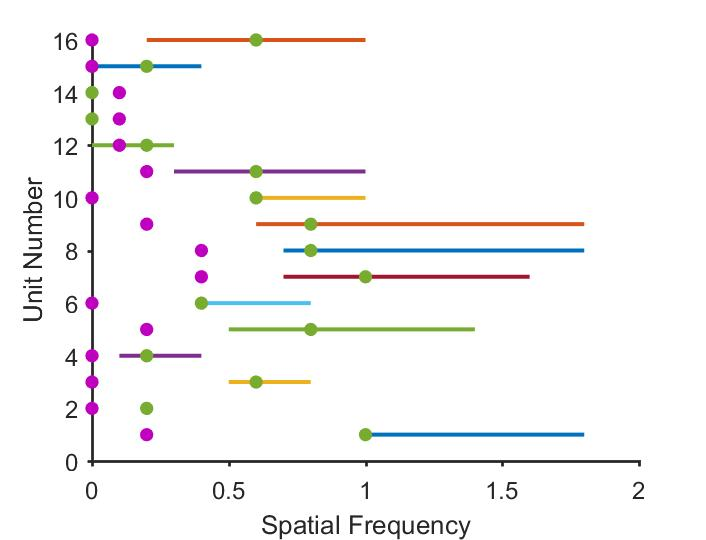
\includegraphics[width=\linewidth]{superiorcolliculus/sf_bandwidth.jpg}
		\caption{The difference between the cut-off frequencies
			for the optimum and orthogonal orientations for 16 units is shown in the
			above figure. The purple circles are the peak spatial frequencies of the
			respective neurons and the green circles are the spatial frequency where
			the cell is most tuned to orientation. In most cases, the neurons are
			most tuned for orientation at spatial frequencies well past the peak
			spatial frequency.}
		\label{fig:sf_bw}			
		\end{figure}
	
	\subsubsection{Modulation Index of the neurons.}
	
For the 16 units whose spatial frequency tuning were recorded, the
distribution of modulation ratios is presented in figure 11. A
modulation ratio less than one means that the modulated component of the
response was lower than the unmodulated component (non-linear cells)
while a modulation ratio of greater than 1 indicates that the neurons
were linear. The median value of the modulation index was 0.76 (95\% CI=
{[}0.65, 1.03{]}) suggesting that most neurons in our sample showed
non-linear summation over their receptive fields.
	
	\begin{figure}[H]
		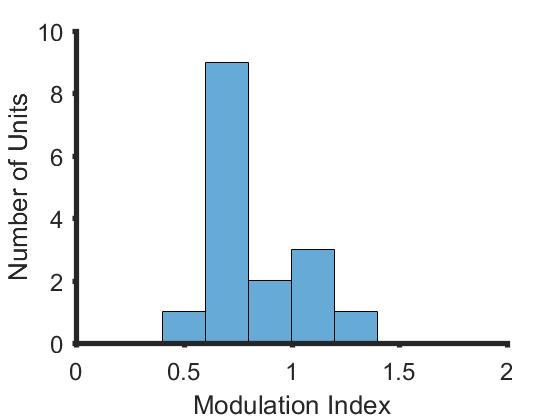
\includegraphics[width=\linewidth]{superiorcolliculus/modulation_index.jpg}
		\caption{The distribution of modulation indices of the
			neurons in our sample. Most neurons had a modulation index less than 1.}
		\label{fig:sc_mi}			
	\end{figure}
	\pagebreak
	\section{Discussion}
Our results show that the majority of neurons in the superficial layers
of the tree shrew SC show orientation biases when tested with bar
stimuli. When tested using grating stimuli, most neurons also showed low
pass spatial frequency tuning and demonstrated orientation tuning at
higher spatial frequencies. We also found that a small proportion of
neurons were tuned to direction and the majority of neurons showed
non-linear summation over their receptive fields.

We used bars to study the orientation selectivity of neurons in the
superior colliculus and found that most units (90\%) were biased for
orientation. We calculated two measures of orientation selectivity the
circular variance and bias. Neurons with a bias greater than or equal to
3 were comparable to the elongated receptive field units previously
reported (Albano et al., 1978). Six out of twenty-two neurons (27 \%)
had a bias greater than 3. This is comparable to the proportion of
elongated receptive field units (19\%) that were reported by Albano et
al (1978). Most of the elongated receptive field units reported by
Albano et al (1978) were found in the lSGS and SO layers and none were
recorded from the uSGS. In our sample, most neurons were biased for
orientation to some degree and neurons that had a bias greater than 3
were found in both the upper and lower SGS with the sharpest tuned
neurons found in the uSGS. We only recorded from one neuron in the SO
which had a bias value of 2.85. This discrepancy in the detection of
orientation biased neurons in the uSGS may be due to the thickness of
the bar stimulus used.

Neurons in the subcortical areas show more tuned responses when shown
thinner bars and at higher spatial frequencies (Vidyasagar and Urbas,
1982; Levick \& Thibos, 1980; Levick \& Thibos, 1982). In response to
gratings, at the peak spatial frequency, the SC neurons showed minimal
orientation biases and the orientation tuning of neurons were usually
more evident at higher spatial frequencies. As a result, if Albano and
colleagues used thicker bars than we have, they may have failed to find
neurons that had elongated receptive fields in the uSGS.

When the spatial frequency tuning of SC neurons and the LGN neurons in
the tree shrew were compared, both LGN and SC neurons showed low pass
spatial frequency tuning. However, when compared to the LGN neurons (as
published in Van Hooser et al., 2013), the peak spatial frequencies we
observed were lower. This could be related to the type of neurons the SC
neurons get their inputs from. SC neurons in most species receive inputs
from achromatic Y-like or W-like cells (DeMonasterio, 1978; Shapley \&
Perry, 1986; Schiller \& Malpeli, 1977; Bunt et al., 1975; Leventhal et
al., 1981). These cells show non-linear summation over their receptive
fields and tend to have lower peak spatial frequencies (Enroth-Cugell \&
Robson, 1966; Derrington \& Fuchs, 1979; So \& Shapley, 1981). Our
results indicate that the SC neurons show non-linear summation (as Y and
W cells do) over their receptive fields while the LGN neurons tended to
show more modulated responses, typical of X-like neurons (Van Hooser et
al., 2013). This could explain the difference in the peak spatial
frequency of the neurons from the two sub-regiongs. One other difference
between the LGN and the SC spatial frequency tuning curves was the high
spatial frequency cut-offs. The SC neurons generally tended to have
higher spatial frequency cut-offs compared to the LGN neurons. A
possible reason could be that in our study, we carefully tested the
responses of the neurons to stimuli of different spatial frequencies to
ensure that the neurons could resolve gratings of higher spatial
frequencies. If uncorrected refractive errors were present in the tree
shrews in the study by Van Hooser and colleagues, then this could
explain the difference in the high cut-off values reported between the
LGN and the SC.

Most neurons in the tree shrew superior colliculus were not tuned to
direction. Van Hooser et al reported that only one neuron in their
entire sample was tuned to direction using DCV in the geniculo-striate
system of tree shrews. Using the same measure, we found that none of our
neurons exhibited direction selectivity. A larger sample may show a
small proportion of neurons being tuned for direction using the DCV in
the superior colliculus. In their study, Albano and colleagues reported
that a proportion of the elongated receptive field cells were also
selective to direction of movement and that these cells were found in
the lSGS and the SO. However, the proportion of neurons tuned to
direction was not reported. Using a less conservative measure than the
DCV, the DSI, we found that approximately 20\% of the neurons were tuned
to direction. Of the 5 direction selective neurons, 2 were from the uSGS
(13\% of the uSGS neurons) and 3 were from the lSGS (50\% of the lSGS
neuons) suggesting that direction selective neurons were sparser in the
uSGS when compared to the lSGS.

In their study, Albano et al., (1978) proposed that the uSGS and the
lSGS could play different functional roles. They found that the uSGS
neurons were composed of only one type of neuron (the stationary
--responsive type) while the lSGS consisted of a combination of
different type of neurons. This claim was supported by anatomical and
morphological evidence; namely, uSGS neurons were generally smaller (5-8
μm) and received predominantly retinal inputs and lSGS neurons were
larger (8-12 μm) and received inputs from both the retina and the cortex
(Abplanalp, 1971). A later study however showed that the retinal inputs
dominated the SGS of the tree shrews with the uSGS receiving less
cortical inputs than the lower SGS. (Graham \& Casagrande, 1980). We
found that the uSGS contained the sharpest tuned neurons in our sample
and a smaller proportion of these neurons were tuned to direction
whereas, all the neurons in the lSGS were broadly tuned to orientation
and a higher proportion of neurons were tuned to direction. When
compared to Albano et al., we found more diverse response properties in
the uSGS rather than the lSGS (e.g.: see figure 4c). However, our sample
size in the lSGS was small (6 uSGS neurons) and any lack of diversity in
the neuronal responses could be attributed to sampling errors.

In this study we found that neurons in the superior colliculus were
tuned to orientation at higher spatial frequencies. Most neurons were
low pass tuned to spatial frequency and at the peak spatial frequency, a
similar proportion of neurons were biased for orientation in the LGN as
well as the SC. In the SC, neurons were sharply tuned to orientation at
higher spatial frequencies. This result is consistent with that observed
in the retina and the LGN of cats and macaques. Layer 4 neurons of the
tree shrews, which resemble LGN neurons (Van Hooser et al., 2013), also
respond similarly at higher spatial frequencies (See Chapter 5). This
similarity in subcortical orientation response across both the
geniculo-striate system as well as the SC indicate that orientation
biases observed in the LGN and the SC could be inherited from the
retina. In the tree shrew then, sharp orientation tuning observed in the
supra-granular layers could be due to the sharpening of orientation
biases by intra-cortical inhibition rather than through Hubel and Wiesel
like excitatory convergence.
	
	\chapter{Is the tree shrew primary visual cortex a linear filter?}
\pagebreak
	\section{Summary}
	It has been contentious whether simple cells in the primary visual cortex (V1) perform patch by patch Fourier Analysis on the visual scene. It has been suggested that if V1 neurons perform patch-by-patch Fourier Analysis, then the receptive field sizes will remain constant. If this is the case, then to obtain the range of peak spatial frequencies reported for the same visual field, the neurons will have different number of sub-regions. Alternately, different peak spatial frequencies can also be obtained by keeping the number of sub-regions the same and changing the receptive field sizes. In this chapter, we will examine which of the above models best explain the receptive field properties of tree shrews. We measured the spatial frequency tuning curves of the neurons and calculated absolute and relative bandwidths. We found that the relative bandwidth was negatively correlated with the peak spatial frequency, suggesting that the shrew V1 neurons, while not ideal, are far better Fourier Analysers than the macaque V1.
	\pagebreak
	\section{Introduction}
	In their seminal paper, Hubel and Wiesel divided cortical neurons into simple and complex cells. While both these types of neurons were orientation selective, they were different in some key ways. Specifically, Hubel and Wiesel described simple cells as neurons that have
	a) spatially segregated on and off regions, 
	b) summation within each region, 
	c) had ON and OFF subregions that were antagonistic 
	d) it was possible to predict the neuron’s response to any stimulus
	Complex cells were neurons that did not have the above properties. In recent years, this has been interpreted as simple cells being linear, X-like neurons while complex cells exhibit non-linear, Y-like responses. 
	It was proposed by Robson and Campbell that neurons in the primary visual cortex function do not all function as a single detector. Rather, they suggest that there are a number of “independent detector mechanism” each of which is tuned to a narrow range of frequencies (Campbell and Robson, 1968).  They also report that there are individual “channels” for most of the spatial frequencies that the neurons see. as patch by patch Fourier transformers. What this essentially meant was that neurons analysed each patch of the visual field individually and extracted the spatial frequency information and then used this information to create a composite whole. Campbell and Robson reframed this hypothesis to say that this implied that neurons that analysed the same patch of visual field had the same receptive field sizes but different peak spatial frequencies. This is supported by studies that have shown that in the primary visual cortex, while there are orientation columns where the orientation remains constant, there are no such spatial frequency columns. Within an area of the cortex, spatial frequency can vary by a lot.
	For neurons to have the same receptive field size but different peak spatial frequencies, they should have different number of receptive field sub-regions. Blah blah blah showed that the size of the receptive subregions affect the peak spatial frequencies whereas the number of receptive field sub-regions affects the bandwidth of the tuning (see figure 1a ). This implies that if the receptive field size remains constant, the only way we could achieve different peak spatial frequencies will be by changing the size of the sub-regions. This would mean that as the peak spatial frequency increases, the size of subregions decrease and the number of sub-regions increase which also means that the spatial frequency tuning bandwidth gets narrower (rows 1 and 2 of figure 1). Alternately, we could achieve the same results by keeping the same number of sub-regions but by changing receptive field sizes as shown in figure 1b and c. In this case, the relative bandwidth of the spatial frequency tuning would remain constant even as the peak spatial frequency increases. In the cats and macaques, this second model of constant relative sub-regions has been shown to be true (Vidyasgar and Kulikowski, 1986; Kulikowski and Bishop, 1981).
	In the tree shrews, while orientation selectivity has been widely studied, very few studies have been conducted on the spatial frequency selectivity of the tree shrew V1. One study looked at the distribution of spatial frequency between layers 2/3 and layer 4 and found that most neurons in layer 2/3 showed band-pass spatial frequency tuning with neurons predominantly showing a tuning bandwidth of 2 octaves. Apart from this one study, no other reports of spatial frequency tuning has been shown. Our own results are similar to previously reported results on the layer 2/3 neurons (see Previous chapter). We also found that compared to layer 4, more neurons were likely to be band-pass tuned for spatial frequency. Here we aimed to examine the relationship between the orientation tuning bandwidth and the peak spatial frequency.
	
	\begin{figure}[H]
		
		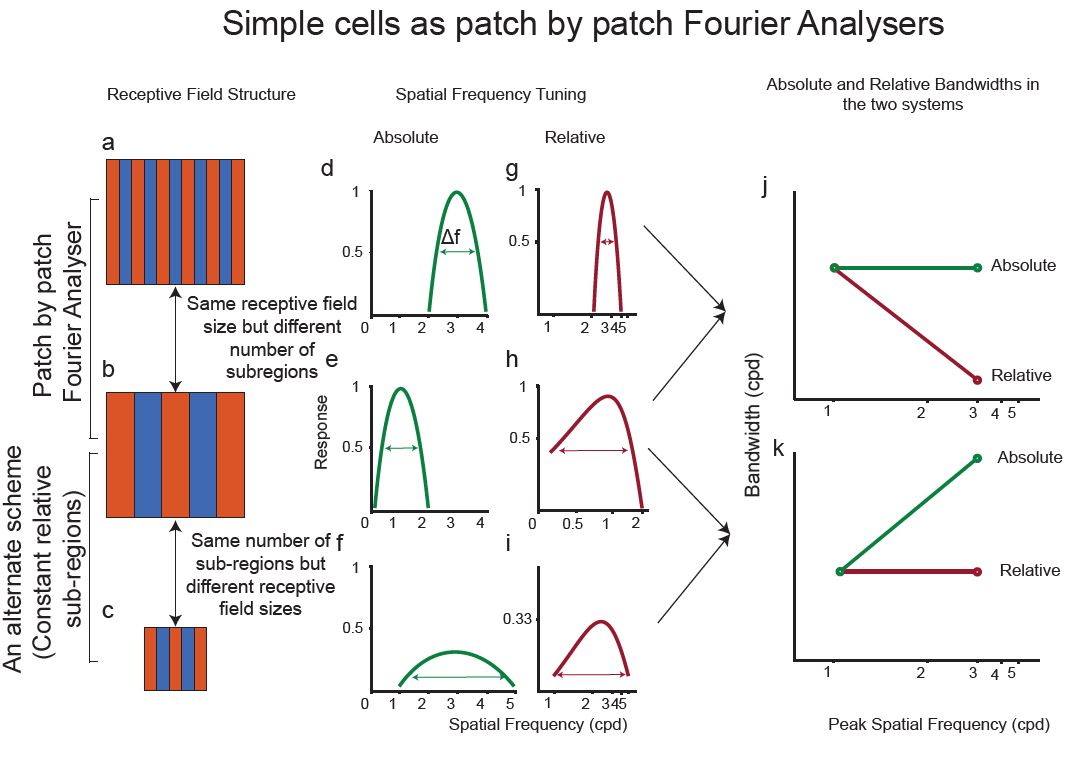
\includegraphics[width=\linewidth]{LinearV1/scheme.jpg}
		\caption{Distribution of segregation indices of neurons.}
		\label{fig:summary}
	\end{figure}

	As mentioned earlier, neurons in the primary visual cortex can be classified as simple or complex cells. The criteria mentioned by Hubel and Wiesel (1962) are all subjective methods of classifying cells into simple cells. Since then, more objective methods of classifying receptive fields into simple and complex have been established. The first method is by calculating the modulation index (MI). The MI is the ratio between the DC and first harmonic component of the temporal modulation neurons exhibit when shown drifting gratings. This method quantifies the “linearity” of a neurons response based on the assumption that simple cells show linear summation within their receptive field sub-regions. Skottun et al (1991) showed that this method successfully divided neurons into two groups which were roughly the same as simple and complex cells divided using the criteria specified by Hubel and Wiesel (1962).
	While the modulation index measured the linearity of the neurons in cats, in macaques and tree shrews, it tended to overestimate the number of simple cells found. In tree shrews, while over 40\% of neurons could be classified as simple using the modulation index, these neurons did not show the segregation of receptive field sub-regions requisite of simple cells (Van Hooser et al., 2013; Veit et al., 2014). This has also been shown to be the case in macaques (References). 
	Further, it has also been suggested that linearity is not a requisite feature of simple cells. Neurons in the LGN maybe classified as X, Y and W cells. While X cells show linear sustained responses, Y cells exhibit transient, non-linear responses. While originally thought that X and Y cells projected to simple and complex cells respectively, this connection has since been disproved. As a result, significant non-linearities may be introduced in simple cells depending on the type of input that they receive. Further, if simple cells do function as edge detectors rather than linear filters, they are unlikely to be linear neurons (DeValois and Webster, 1978). Hence, alternate methods of classifying simple cells are also examined below. 
	Whether there are cortical simple and complex cells have also been debated. Depending on stimulus parameters, there seems to be a continuum of neurons rather than a bimodal distribution of neurons in the primary visual cortex. So the linear component of all neurons have also been subjected to the same analysis.
	
	\section{Methods}
		
		\subsection{Surgery and Anaesthesia}
		Surgical procedures are as outlined in the Methods chapter. Briefly, the animal was anaesthetized using a mixture of Ketamine and Xylazine, a venous catheter was inserted in to the femoral vein and a tracheostomy performed to assist in breathing during the experiment. The animal was administered muscle paralysant (Vecuronium Bromide) intravenously and was anaesthetised using Isoflurane (0.5-1\%) for the duration of the experiment. Hard contact lenses were fitted to the eye to prevent corneal drying. In some tree shrews, additional lenses were used to correct for any refractive errors. A craniotomy and durotomy were performed over the location of V1 (Horsley-Clarke Co-ordinates A2.5 to P2.5). ECG and frontal EEG were monitored during the experiment. At the end of the experiment, the animal was euthanized using an overdose of pentobarbital sodium and perfused using 0.1M Phosphate Buffer (PB) solution followed by 4\% Paraformaldehyde in 0.1M PB. The brain was removed and stored in sucrose (20-25\%) for histology.
	
		\subsection{Electrophysiology}
		High impedence, lacquer coated tungsten microelectrodes (FHC Metal Microelectrodes Inc., ME, USA; impedance= 12-18 MΩ) were lowered into the brain at an angle perpendicular to the cortical surface. The signal was amplified and filtered (x 10,000 gain, bandpass filtered between 300-3000 Hz, A-M systems) and fed into an audio speaker as well as an analog to digital converter (Cambridge Electronic Design Limited, Cambridge, UK; digitised at 22.5 kHz). Neurons were recorded from Layers 2/3 and Layer 4. Layer 4 could be identified by a characteristic ‘swish’, first for on stimuli and then for off stimuli, in the tree shrews. Where we no longer heard the swish, we concluded that we exited layer 4 and into layer 5. Neurons in layers 5 and 6 were not recorded from. Lesions (6 μA for 6s) were made at the end of each track. The electrode was withdrawn and lesions were made at regular intervals to trace the path of the electrode through the brain. The data was recorded as a spike trace using the spike 2 software (CED, Cambridge, UK). The spikes were templated and the spike timing exported as a text file. Further analysis was performed using custom MATLAB code (The Mathworks Inc, USA).
		\subsection{Stimuli}
		A hand-held projectoscope was used to mark the receptive field boundaries. Using this, the centre of the monitor was aligned with centre of the receptive field prior to stimulus presentation. Stimuli were presented using a BARCO monitor (Frame Refresh Rate= 80 Hz; Reference Calibrator Plus; Barco Video and Communications, Belgium) and generated using Visage (VSG, Cambridge Research Systems, Cambridge, UK) and custom Stimulus Description Language (SDL) scripts. The monitor had a mean luminance of 32.6 cdm-2. While recording, the monitor was placed at a distance of 114 cm from the eye. For each of the different stimuli described below, ten complete stimulus presentations were completed.
				\subsubsection{Bar Stimuli}
				For each neurons, an initial estimate of optimum orientation was obtained using bars, moving bi-directionally across the screen. The background was a uniform gray screen. Depending on the polarity of the neurons, either a bright bar or a dark bar was used (contrast= 100 \%). The bar was usually 8o long (ranging between 4 and 8 degrees) and 0.5o wide (ranging between 0.1 and 1 degree). A total of 18 different orientations were tested and PSTHs (see methods) were made online using the Spike 2 software. The orientation that yielded the highest firing rate was used for further testing.
				After determining optimum orientation, bidirectional, dark and light (decreasing and increasing contrast) bars of the optimum orientation were used to get the response profile of the neurons to opposite polarities (see Fig. 1). 
				\subsubsection{Grating Stimuli}
				For all neurons, once optimum orientation was determined, spatial frequency tuning of the neurons were studied. Drifting sine-wave gratings (TF= 4Hz, Contrast=100\%) of increasing spatial frequencies (between 0 and 2.2 cpd) and in the optimum orientation were presented to neurons. The responses were recorded and stored for further analysis.
				
   		\subsection{Data Analysis}
		Regardless of the stimulus presented, the following analysis was performed on the extracellular trace before any specific analysis was undertaken. Spikes were templated and the spike time and stimulus markers were exported into text files. Using custom scripts in MATLAB, PSTHs (bin-width= 20ms) were constructed for each of the stimulus conditions.  Spike density functions were created using a moving Gaussian envelope with σ of 60 ms (3 bins). This SDF was used for further analysis. 
				\subsubsection{Analysis of Bar Stimuli Responses}
				Orientation tuning was analysed and presented in an earlier chapter. Here is the method by which the dark and light bar data was analysed.
					\paragraph{Calculating Segregation Index (SI)}
					For neurons where dark and light bar data was available, the segregation index (SI) was calculated using the following formula: 
					\[SI=\frac{\sum|R_ton-R_toff|}{\sum|R_ton+R_toff|}\]
					Where, R\_ton is the response of the neuron to a light bar and R\_toff is the response of the neuron to a dark bar (see figure 1). The resulting value was a number between 0 and 1. Neurons with high segregation index (>0.5) were more likely to have segregated dark and light sub-regions and were hence categorised as simple cells. Likewise, neurons with low segregation indices were classified as complex cells as they were less likely to have segregated dark and light sub-regions.
				
				\subsubsection{Analysis if Grating Stimuli Responses}
				
				For all neurons, a discrete fourier transform was applied to the PSTH using the MATLAB fast fourier transform algorithm (FFT). The DC (F0) and the first harmonic component (F1) of the response was used for further analysis. Optimum spatial frequency for the neurons was determined as explained in Chapter 4. The modulation ratio was then calculated as follows.
				
				\[Modulation Index (MI)= 2*\frac{F_1}{(F_1+F_0)}\]
				
				Where Rf1 and Rf0 are the responses of the F0 and F1 components at the peak spatial frequency.
				The modulation ratio returned a number between 0 and 2. If the neuron had a modulation index greater than 1, it was classified as simple and it was classified as complex otherwise (Van Hooser et al., 2013). Only neurons classified as simple cells were used for further analysis and only the F1 component of the responses were further analysed.
				For each neuron, two spatial frequency tuning bandwidths were calculated. One was the absolute bandwidth which was the difference between the upper and lower cutoff spatial frequencies. The upper cut off was calculated as the spatial frequency greater than the peak spatial frequency where the response first reaches half the maximum response. The lower cutoff was calculated similarly for spatial frequencies lower than peak spatial frequency where response first reached half the maximum response. If the response never reached half the maximum response, the neuron was classified as low pass or high pass tuned. The relative bandwidth was then calculated as the absolute bandwidth/ peak spatial frequency.
				
		\subsection{Histology}
				The brains were stained for Nissl substances using cresyl violet acetate and lesions were located. The number of neurons found in each layer have been presented in V1 chapter and are not presented here. However, for all the results presented here, layer specific results are also presented.
							
					

	\section{Results}
	
		Results from a total of 64 neurons are presented below. Where possible, the layerwise distribution is also presented. 
		
	\paragraph {Segregation Index}	
	In 49 of the 64 neurons, we recorded the response of the neuron to dark and light bars. Simple cells have segregated receptive fields which appear as separate peaks in the PSTHs (Fig 1a) and complex cells have overlapping subregions which appear as overlapping peaks in the PSTH (Fig 1b). Accordingly, the segregation index is higher for simple cells compared to complex cells.
	
		\begin{figure}[H]
		
		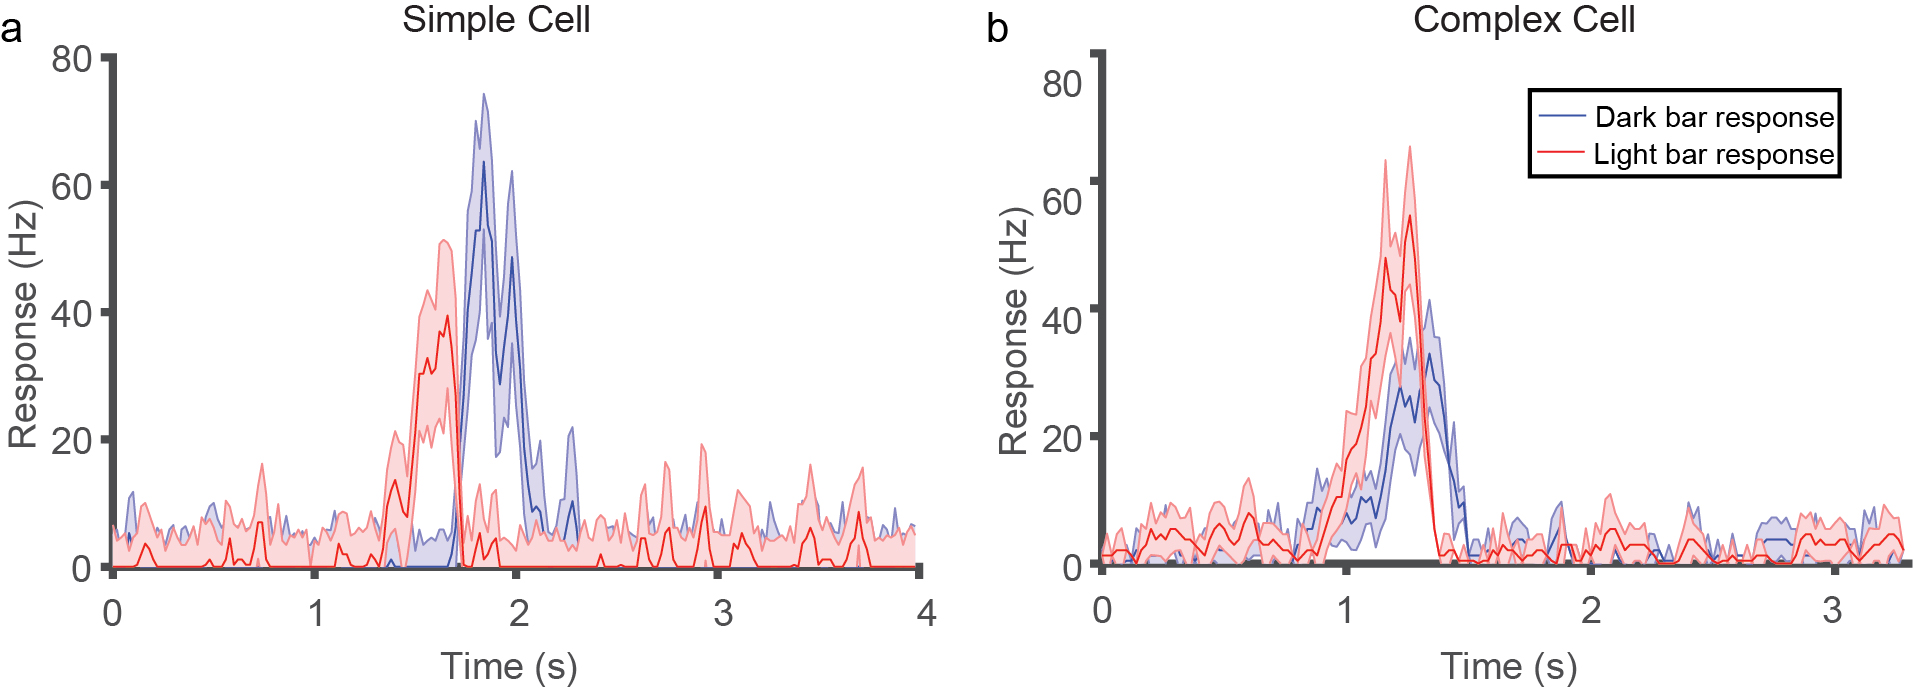
\includegraphics[width=\linewidth]{LinearV1/simplecomplex.jpg}
		\caption{Response of a simple (a) and complex cell (b) to the dark and light bar stimuli. The spatially segregated RF of the simple cells is translated into the temporally segregated response of the neuron. Whereas, in the complex cell, the overlapping sub-regions are reflected in the temporally overlapping response of the neuron. Accordingly, the simple cell has a high SI (0.92) and the complex cell has a lower SI (0.39).}
		\label{fig:fig2}
	\end{figure}
	
	The distribution of segregation index for 47 neurons is presented below. Of the 49 neurons, 19 were from layer 2/3, 12 were from layer 3c and 18 were from layer 4. There was no significant difference in SI between the layers (Kruskal-Wallis test, p=0.34).
	\begin{figure}[H]
		
		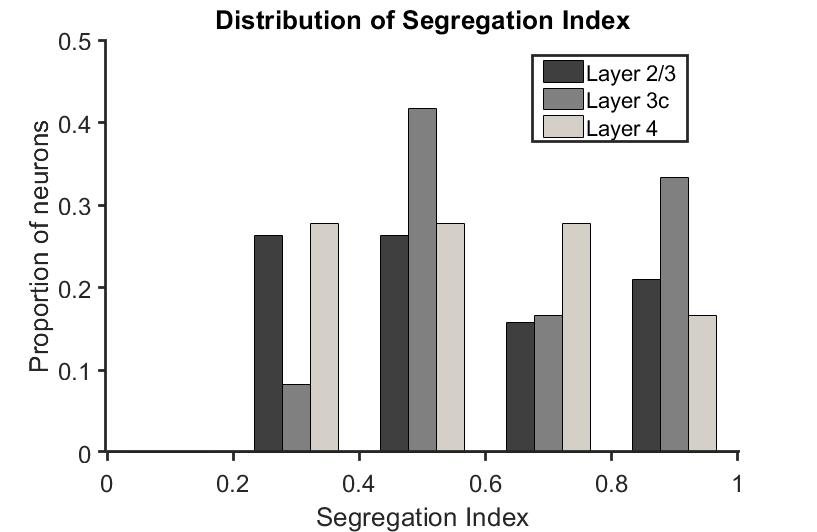
\includegraphics[width=\linewidth]{LinearV1/segregationindex_colouradj.jpg}
		\caption{Distribution of segregation indices of neurons.}
		\label{fig:fig3}
	\end{figure}

	\paragraph{Modulation Index}
	The modulation indices of all the 69 neurons [Layer 2/3= 27; Layer 4= 27; Layer 3c= 15] are shown in figure 3. There was no significant difference in the modulation index between the layers (Kruskal-Wallis test, p= 0.74).
	
		\begin{figure}[H]
		
		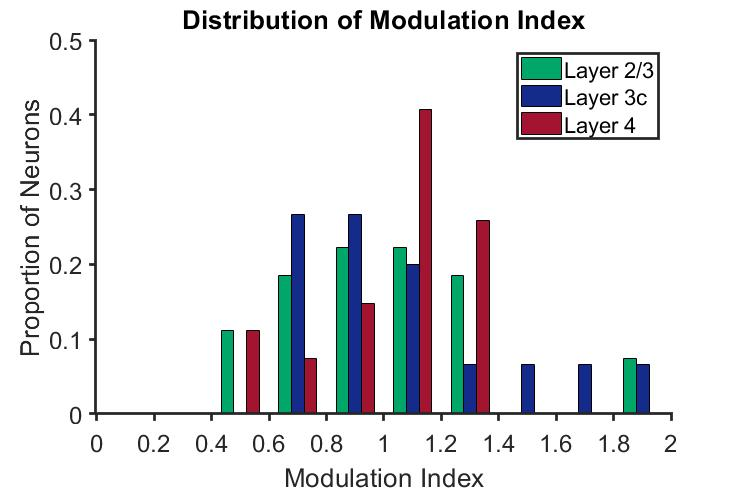
\includegraphics[width=\linewidth]{LinearV1/modind_layer_colour.jpg}
		\caption{Distribution of modulation indices of neurons.}
		\label{fig:fig4}
	\end{figure}
	In neurons where both the segregation index and modulation index were recorded, they were plotted against each other. There was no significant correlation between the two indices (rho=0.02, p=0.89). 
	
	
	\begin{figure}[H]
		
		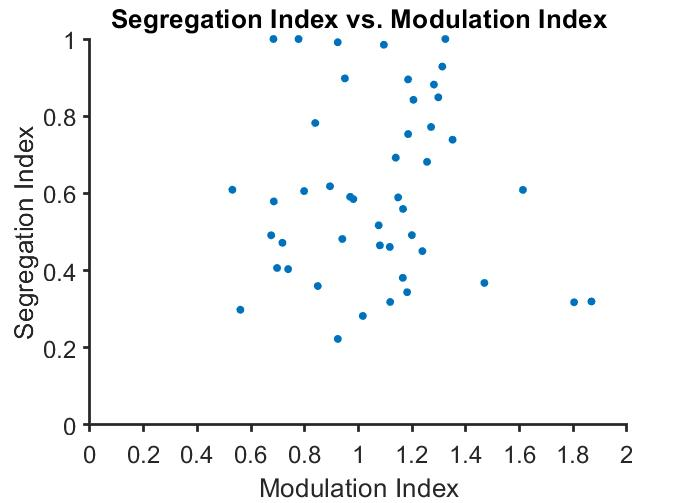
\includegraphics[width=\linewidth]{LinearV1/Segindvsmodind.jpg}
		\caption{Relationship between the modulation and segregation indices.}
		\label{fig:fig5}
	\end{figure}

	\paragraph{Relationship between bandwidth and spatial frequency}
	
	Neurons were classified as simple cells using the modulation index (MI>1), the segregation index (SI>0.5), both the modulation and segregation index together (MI > 1 and SI >0.5). The relationship between the absolute bandwidth and the peak spatial frequency for simple cells classifies as described as above as well as for all the neurons in the sample are shown in figure 5(a,c,,e \& g). Statistically significant relationships are indicated using $*$. For the other two measure used for classification, the correlation was not significant. There was a significant correlation between the when all neurons were used for the analysis. The relationship between relative bandwidth and the peak spatial frequency are shown in the right hand panel. In all cases except for the one in (f) the results were statistically significant.
	
		\begin{figure}[H]
		
		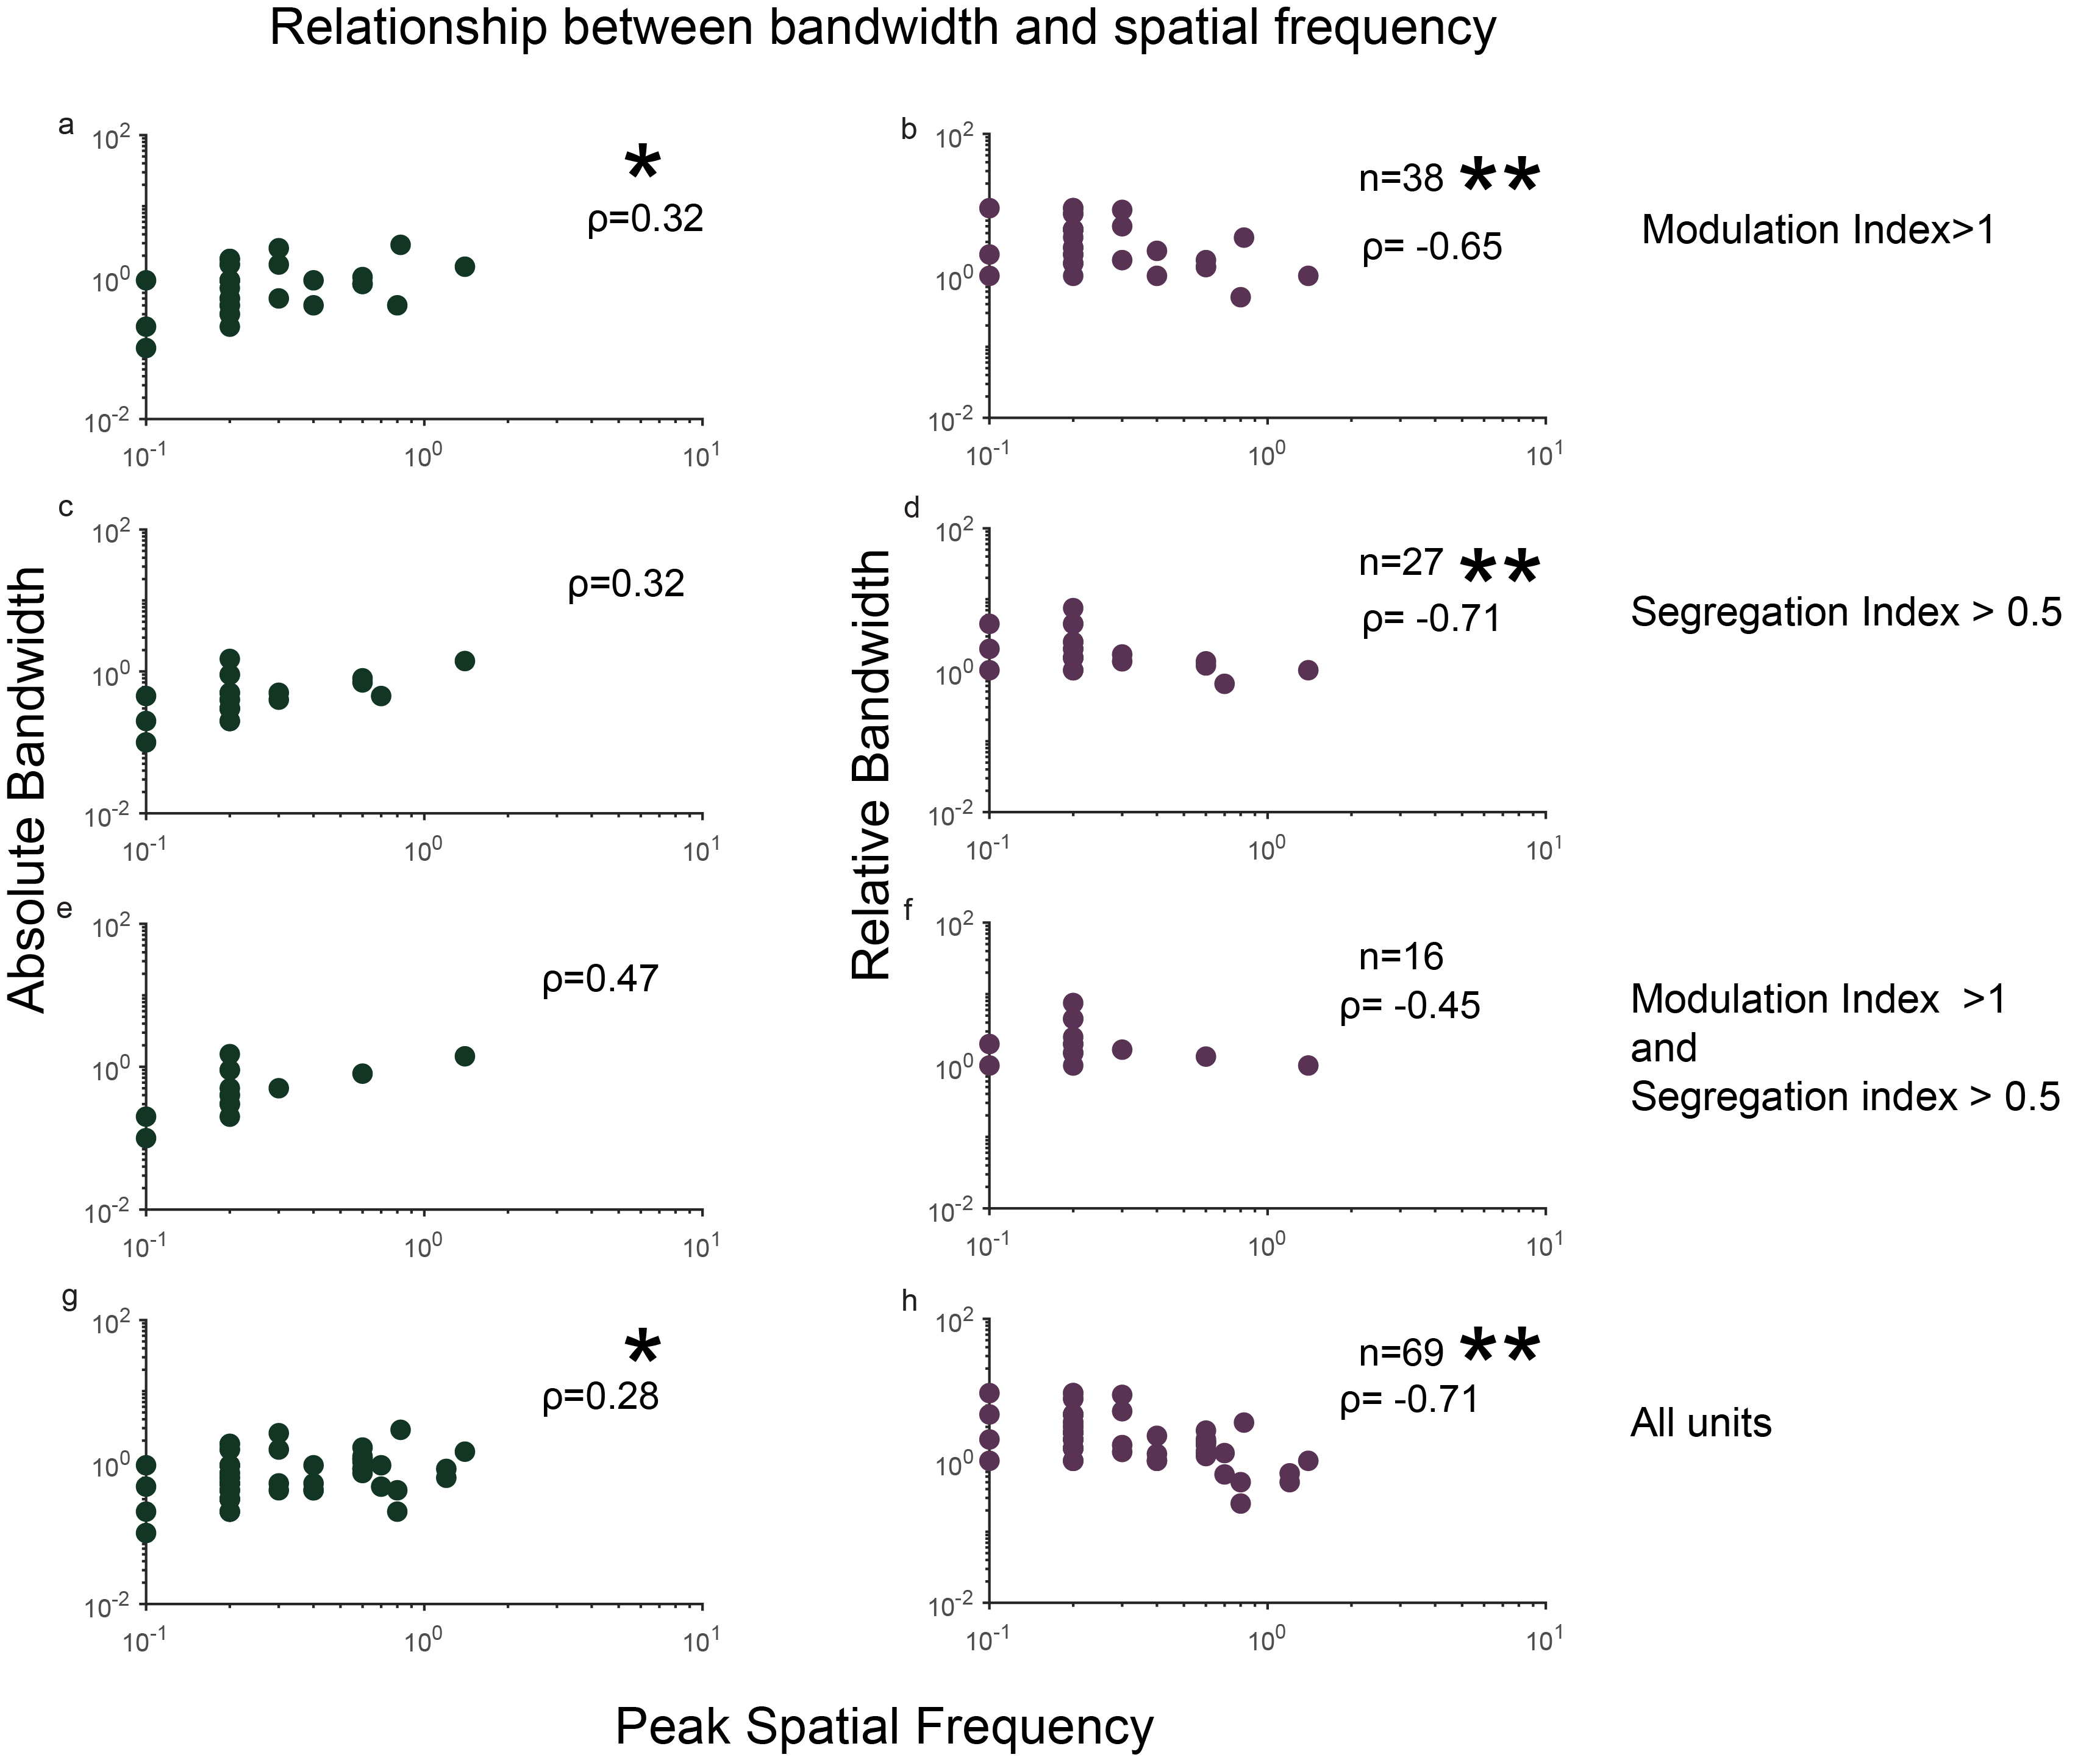
\includegraphics[width=\linewidth]{LinearV1/hwpksf.jpg}
		\caption{This figure shows the relationship between bandwidth and spatial frequency in simple cells when using the modulation index to classify units (a,b), when using the segregation index (c,d); using both the modulation and segregation index (e,f) and for all neurons in the sample (g,h). The plots on the left hand side show the relationship between absolute bandwidth and the peak spatial frequency while the plots on the right hand side show the relationship between the relative bandwidth and peak spatial frequency. Number of units used for generating each plot is specified in the right hand corner and statistically significant results are shown by *. *= p$<$0.05. **=p$<$0.0001.}
		\label{fig:fig6}
	\end{figure}
	
	
	\section{Discussion}
	
	In this chapter, we investigated whether neurons in the tree shrew V1 behaved like patch by patch Fourier analysers. Our results show while most simple cells do not behave like ideal Fourier analysers, they are still far better Fourier analysers than the neurons in cat and macaque striate cortex.
	
	In order to classify the neurons into simple and complex cells, we used two objective measures that are regularly used in the literature: a) The Segregation Index and b) The Modulation Index. The SI measures the degree of separateness of the receptive field sub-regions i.e., if there are separate on and off sub-regions. Using this measure, we found that about half the neurons for which this data was available for were simple. The MI on the other hand measures the degree of linear summation over the receptive fields. Using this measure too, a similar proportion of  neurons were classified as simple cells. However, there was no significant correlation between the two measures (See fig.\ref{fig:fig5}). This indicates that different neurons are classified as simple based on the two different measures. Only half the neurons that were classifies as simple using the SI were also classified as simple using the modulation index, indicating that atleast half the neurons that show linear summation over their receptive field also had overlapping sub-regions. 
	
	Of the neurons that were classified as simple using both MI and SI, there was no statistically significant correlation between the peak spatial frequency and the absolute bandwidth. However, this doesn't necessarily mean that these neurons do not function as Fourier analysers. A power analysis showed that for an expected correlation of -0.45, the sample size had to be atleast 36 for a statistically significant result. It could simply mean that there was not enough neurons in our sample.
	
	The distribution of SI and MI in our results show that neither of these values differ significantly across layers. The SI seems to be distributed almost uniformly across the whole range of possible values (between 0 and 1). However, it is interesting to note that no neurons showed complete and equally overlapping subregions (SI $<$ 0.2; see fig.\ref{fig:fig3}). These results are also consistent with those published by Van Hooser et al., 2013 (see fig 3c). This could mean that most neurons in the shrew V1 receive unbalanced on and off inputs. (Check Bimodality Index). Previous studies have suggested that the tree shrew V1 has a preponderance of off dominated neurons. It has also been suggested that this off dominance could be the origin of orientation selectivity in the V1 of tree shrews. Another reason for the difference could also be the way SI is calculated. The SI is calculated from the temporal profile of the neuronal response to light and dark bars. While this gives an accurate enough measure, it may not be sensitive enough to detect small differences in sensitivities between the off and on regions.
	
	While the distribution of MI was not significantly different between the layers, there are a few important trends that may be of note. First, while the layer 2/3 and layer 3/c distribution look identical, a majority of Layer 4 neurons seem to have a modulation index greater than 1 (see fig.\ref{fig:fig4}). This is consistent with reports in literature where the simple cells are present predominantly layer 4 with some complex cells also found in this layer. However, a significant proportion of layer 2/3 and layer 3c neurons are also highly modulated, simple like neurons, which are reported only rarely in the literature (References). 
	
	Here we used a modified version of the modulation ratio (F1/F0) to quantify the degree of linear summation within the receptive field. In the original modulation ratio, neurons were only classified as simple if their F1/F0 ratio was greater than 1.57 (Skottun et al., 1991; Movshon et al., 1978). This number roughly translates to an MI of 1.2. Therefore, while neurons whose MI are between 1 and 1.2 have a greater modulated component of the response compared to the unmodulated component, they still show significant non-linearities. These neurons have been classified previously as 'b' cells. In our sample, we also found that these neurons were dominated by one polarity (either on or off), which also makes sense as on and off neurons are segregated into layers in the shrew V1.

	Finally, the distribution of SI and MI observed in our data also calls into question the age old question of whether simple and complex cells are two separate categories of neurons or if they lie on a continuum. Our data shows that both these measures are unimodally distributed and not bimodally distributed in line with previous studies which have suggested a similar pattern. Further, it has also been suggested that under certain circumstances, simple could behave like complex cells and complex cells could behave like simple cells. This property of neurons has been implicated in their ability to transmit signals; i.e., simple cells will behave like simple cells when their output is relevant for perception but not otherwise.

	Plan:
	1) Summary of results
		Differences in modulation index and segregation index. What this means? Linearity of neurons?
		Segregation index: no neurons that had completely overlapped sub-regions i.e. si<0.2.
		with the rest of the SI, evenly distributed across the layers.
		There was no significant differences between layers.

		Modulation index: Although not statistically significant, modulation index<1 for most layer 2/3 and layer 3c. modulation index>1. Most layer 4 neurons, have a modulation index between 1 and 1.2. This is the equivalent of between 1 and 1.57 using the standard modulation ratio calculated (F1/F0). These neurons still have a higher modulation index but not high enough. Could be potential B cells described by Henry et al or the non-linear simple cells described by other people. 
		
		Simple cells are found in input layers while complex cells are found in supragranular layers. True if we look at the modulation index but not when looking at the segregation index. Provides support against the heirarchical model of visual processing where simple cells project to complex cells. Also has been shown in other species- complex cells are found in layer 4 and simple cells in supragranular layers. We see the same trend here.
		
		How do our results of segregation index and modulation index compare with the previously published results for segregation and modulation ratios?  Our results are similar to previously published results by Van Hooser et al., 2013. Both results seem to show a unimodal distribution with a range of linearities in the receptive fields when compared to a simple/complex bimodal distribution. Is this because of the measure used for modulation index? Checked with regular modulation index (F1/F0) This measure also did not yield a bimodal distributions.
		
		What does the relative bandwdth and spatial frequency relationship mean?
		
		We found that in most cases, there was a negative relationship between the pk spatial frequency and the relative bandwidth of the neurons, especially when the linear component of all the neurons were used to run the analysis. This means that most neurons in the shrew V1 actually do act as linear filters in optimum range of the neurons (See Fig.\ref{fig:fig1}).
		What exactly does this mean? The cortex could be completely throwing out this information when non-linear?
		
		What is linearity even useful for?
		ARe there simple and complex cells in the shrew cortex? Does this mean anything?
	\chapter{General Discussion}


	
\bibliography{References/library}
 \bibliographystyle{apacite}



\end{document}

